\chapter{Evaluation} 

\section{Methodology}

This section will evaluate the performance of our autoencoder and regression models on unseen images. As explained in Section \ref{subsec:selecting_dataset}, three sets of images were selected for research:

\begin{itemize}
    \item A \textbf{full dataset} containing all categories, with no class imbalance issues
    \item A \textbf{dual dataset}, with no class imbalance issues, containing images from two classes only 
    \item A `\textbf{DMSO-only' dataset}, which should show the most distinction between classes, with class imbalance issues. This dataset did not include any experimental conditions using drugs, only stimulation conditions.
\end{itemize}

Each image in these datasets was categorised by stimulation level: one of \textit{Unstimulated}, \textit{OVA}, or \textit{ConA}. If the image contained image aberrations, it was labelled \textit{Faulty} instead in the case of the autoencoder. In the case of the regression model, the overlap value of \textit{Faulty} images was set to 0. Figure \ref{fig:explain_categories} illustrates what an image from each category looks like.

\begin{figure}[h]
    \centering
    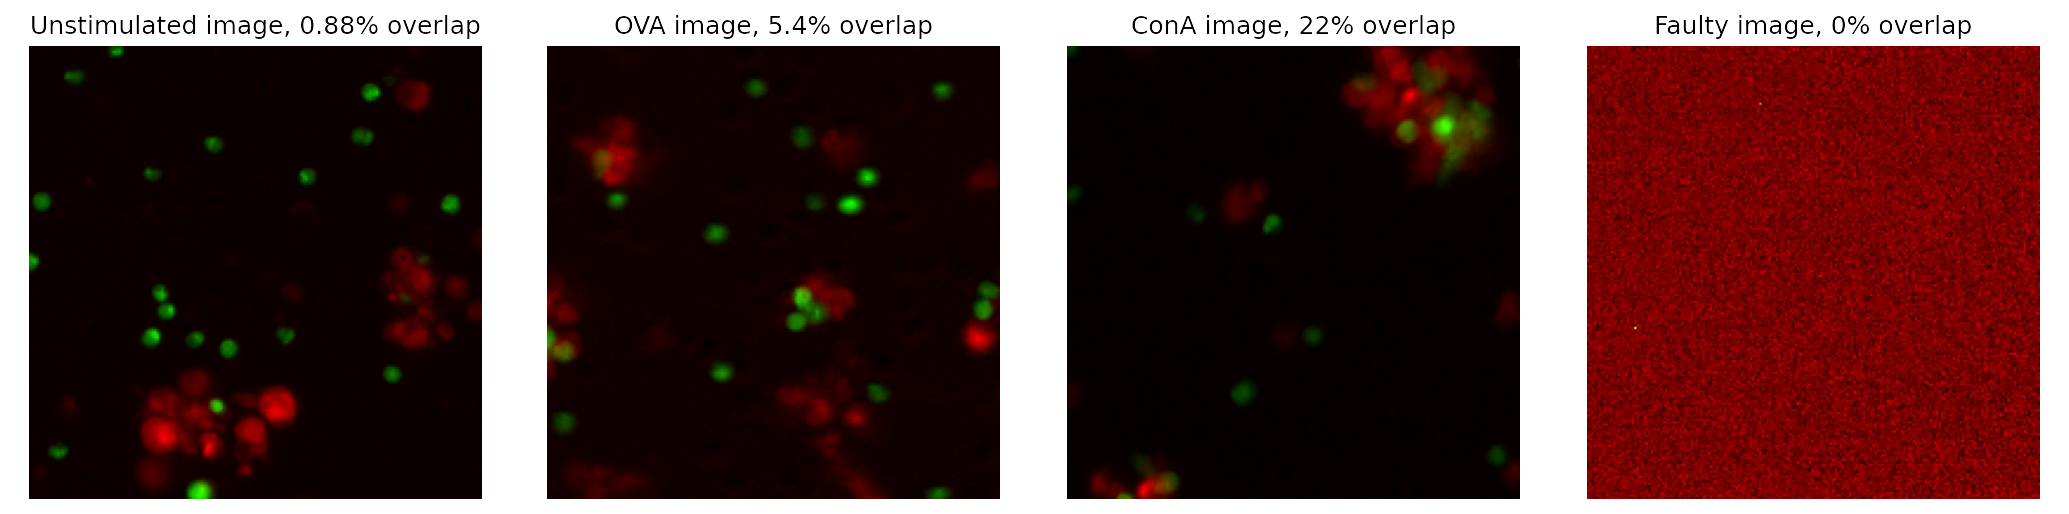
\includegraphics[width=\textwidth]{dissertation/figures/category_images.png}
    \caption{Example validation images taken from each stimulation category. Each image is also labelled with its overlap value. From left to right: \textit{Unstimulated}, $0.88\%$ overlap; \textit{OVA}, $5.4\%$; \textit{ConA}, $22\%$; \textit{Faulty}, $0\%$.}
    \label{fig:explain_categories}
\end{figure}

We had two versions of each dataset: one which had been noise-corrected, and one which had been background-corrected through the help of k-means colour segmentation. This dataset was denominated the `masked' dataset. We trained separate models on those two datasets to evaluate the impact of the background on the model's learning. 

Training and validating was done on the full dataset's 19,000 instances. We had 10,000 instances of this dataset left for testing, and 13,800 instances of the dual dataset, as well as 8,000 instances of the DMSO dataset. All datasets were consistently shuffled before training and testing with the same random state parameter. We made sure there was no overlap between any of the datasets. No image was used for both training and testing. 

The following criteria were chosen in our evaluation:

\begin{itemize}
    \item The success of the autoencoder model will be evaluated on its capacity at image reconstruction, as well as if a UMAP projection of the coded images shows some underlying structure of the data. 
    \item The regression model will be evaluated on how well it predicts overlap values for unseen images of immune cells. 
\end{itemize}

\section{Autoencoder}

\subsection{How well can we reconstruct an image?}

Our autoencoder model is trained on binary cross-entropy loss. The model learns by trying to minimise the difference between two distributions of pixels: the input, and the output. The closer the loss is to 0, the more similar the two distributions are. This means that a score closer to 0 is equivalent to the autoencoder reconstructing an image well. We can use this value as a metric for comparing results between models and datasets. We can also assess the visual quality of an image on reconstruction. 

The following images in Figures \ref{fig:full_reconstruction}, \ref{fig:dual_reconstruction}, \ref{fig:dmso_reconstruction} show how the autoencoder performed on image reconstruction for each of the datasets. The output images were all reconstructed by the model from a 1,152 inner representation of the input image of 110,592 pixels.

\begin{figure}[h!]
    \centering
    \begin{subfigure}[h!]{0.45\textwidth}
        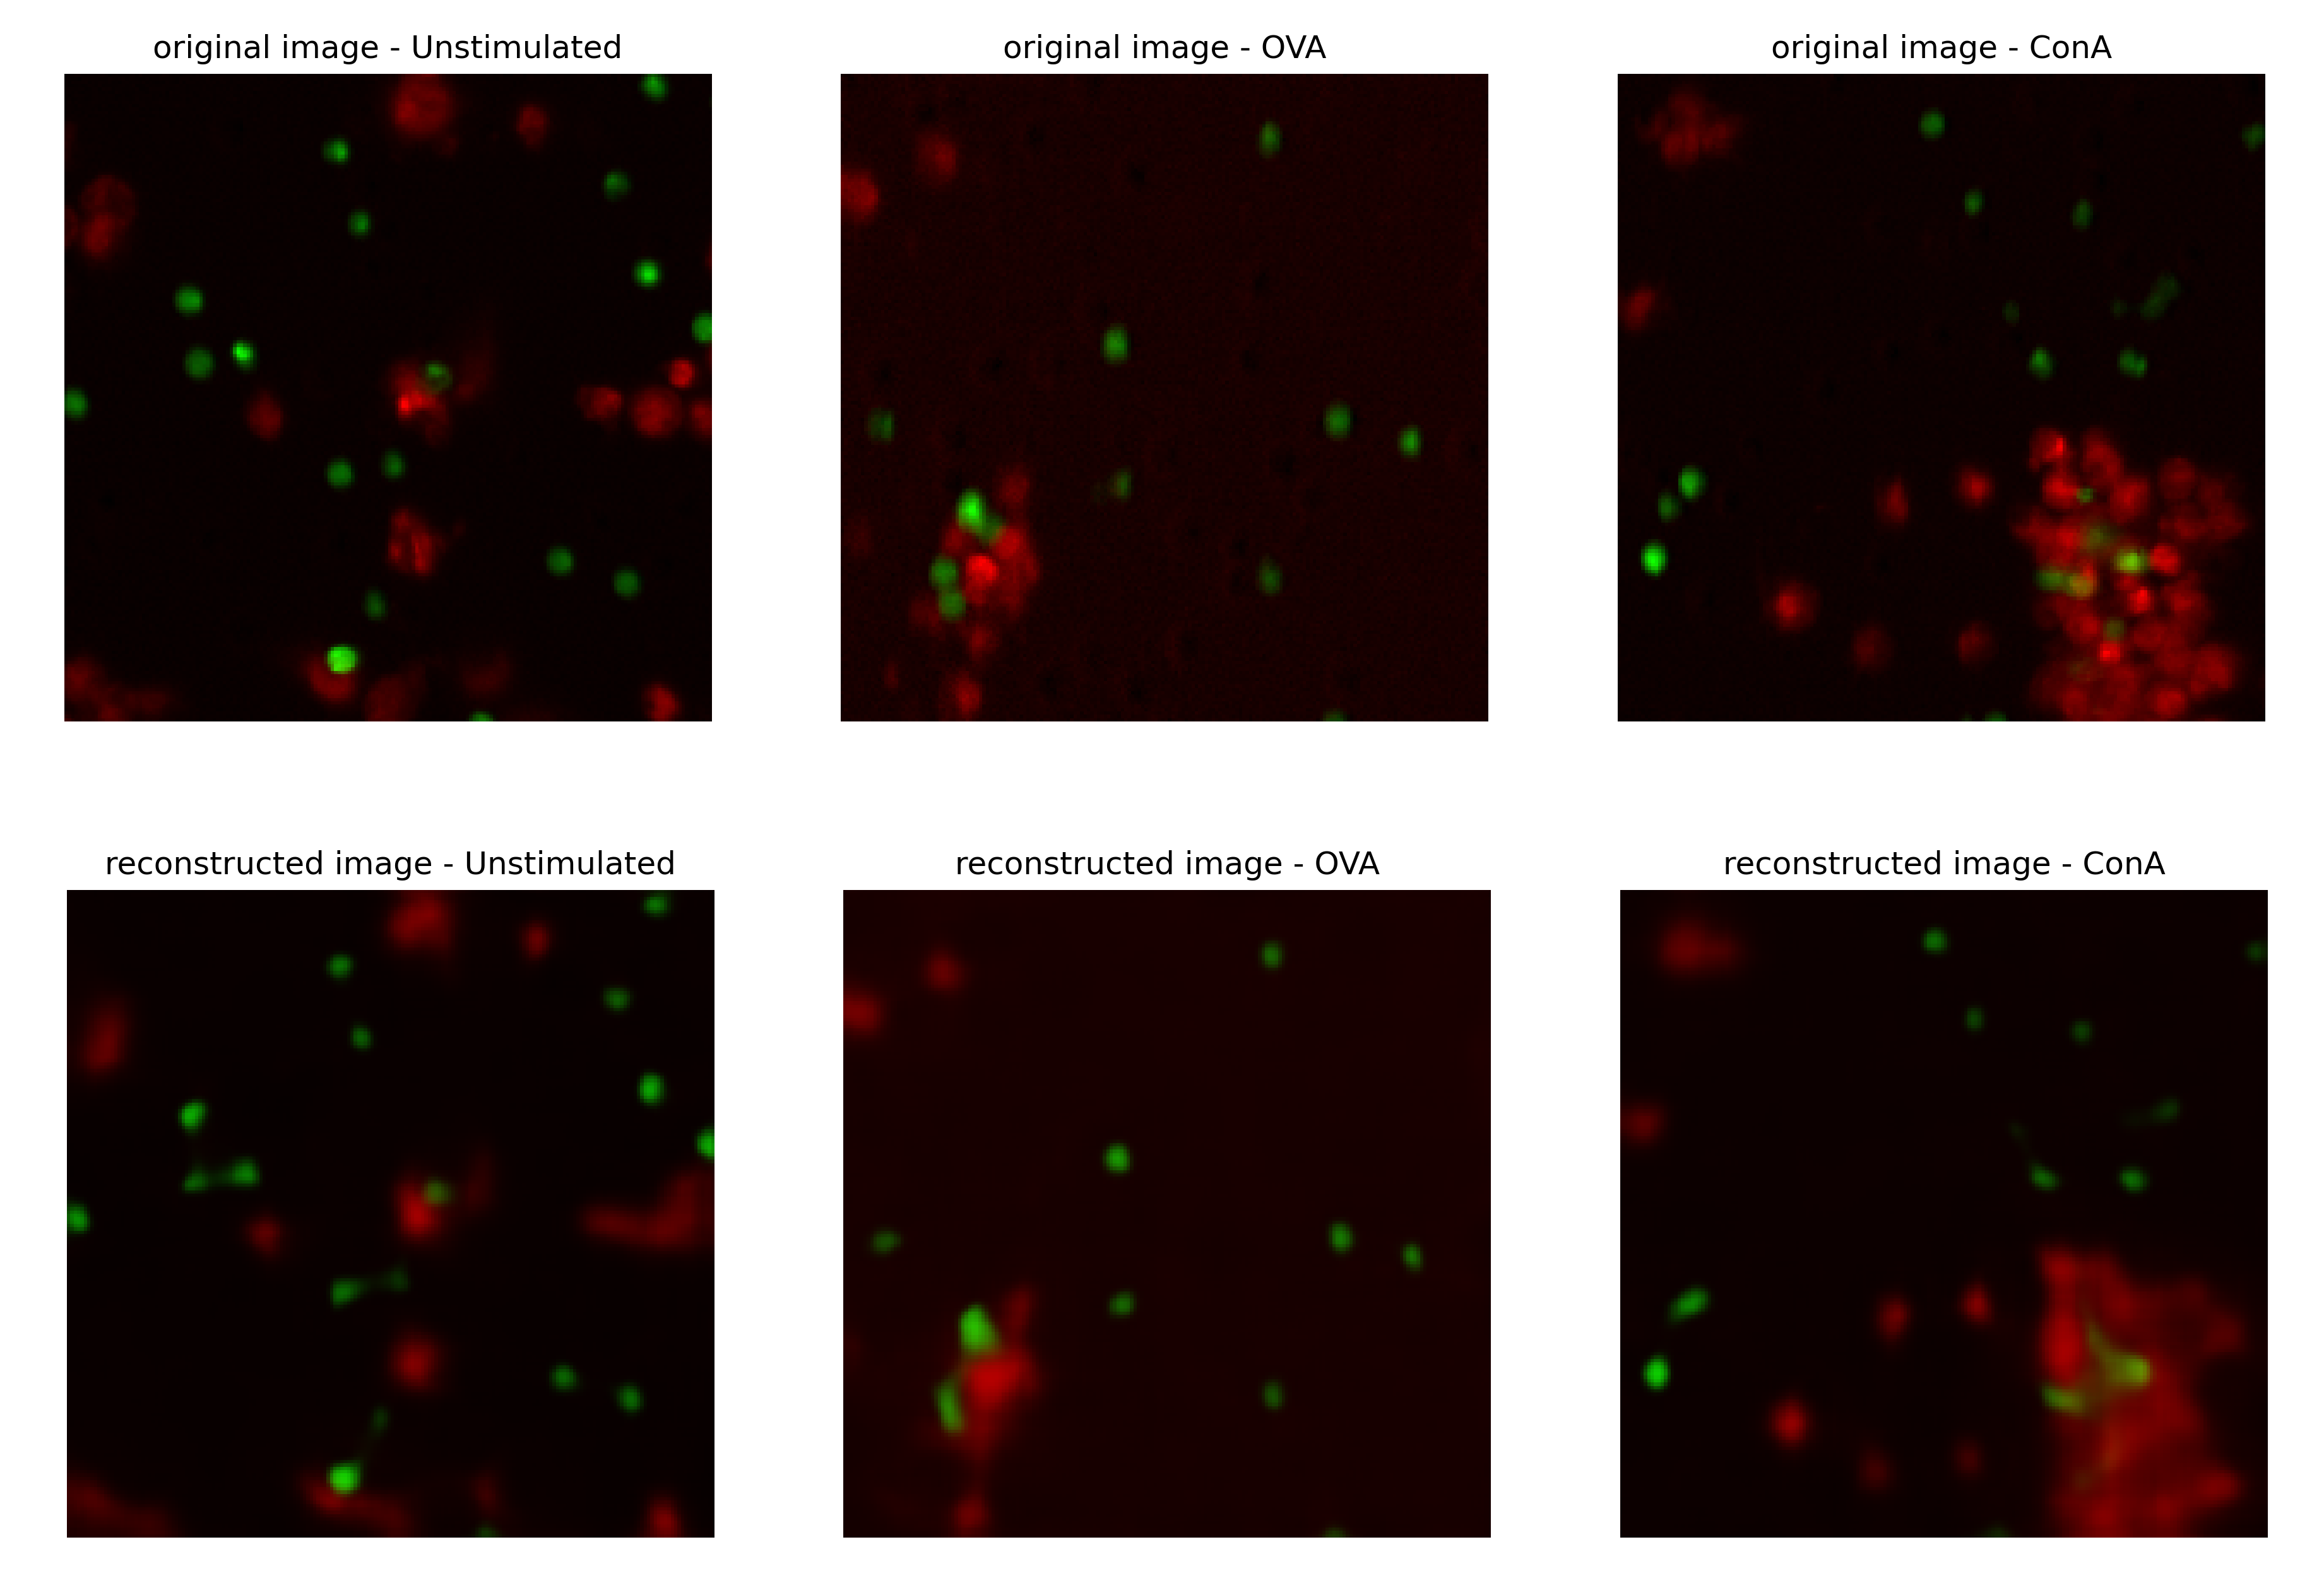
\includegraphics[width=\textwidth]{dissertation/figures/evaluation/CK19_reconstruction.png}
        \caption{Normal images}
    \end{subfigure}
    \begin{subfigure}[h!]{0.45\textwidth}
        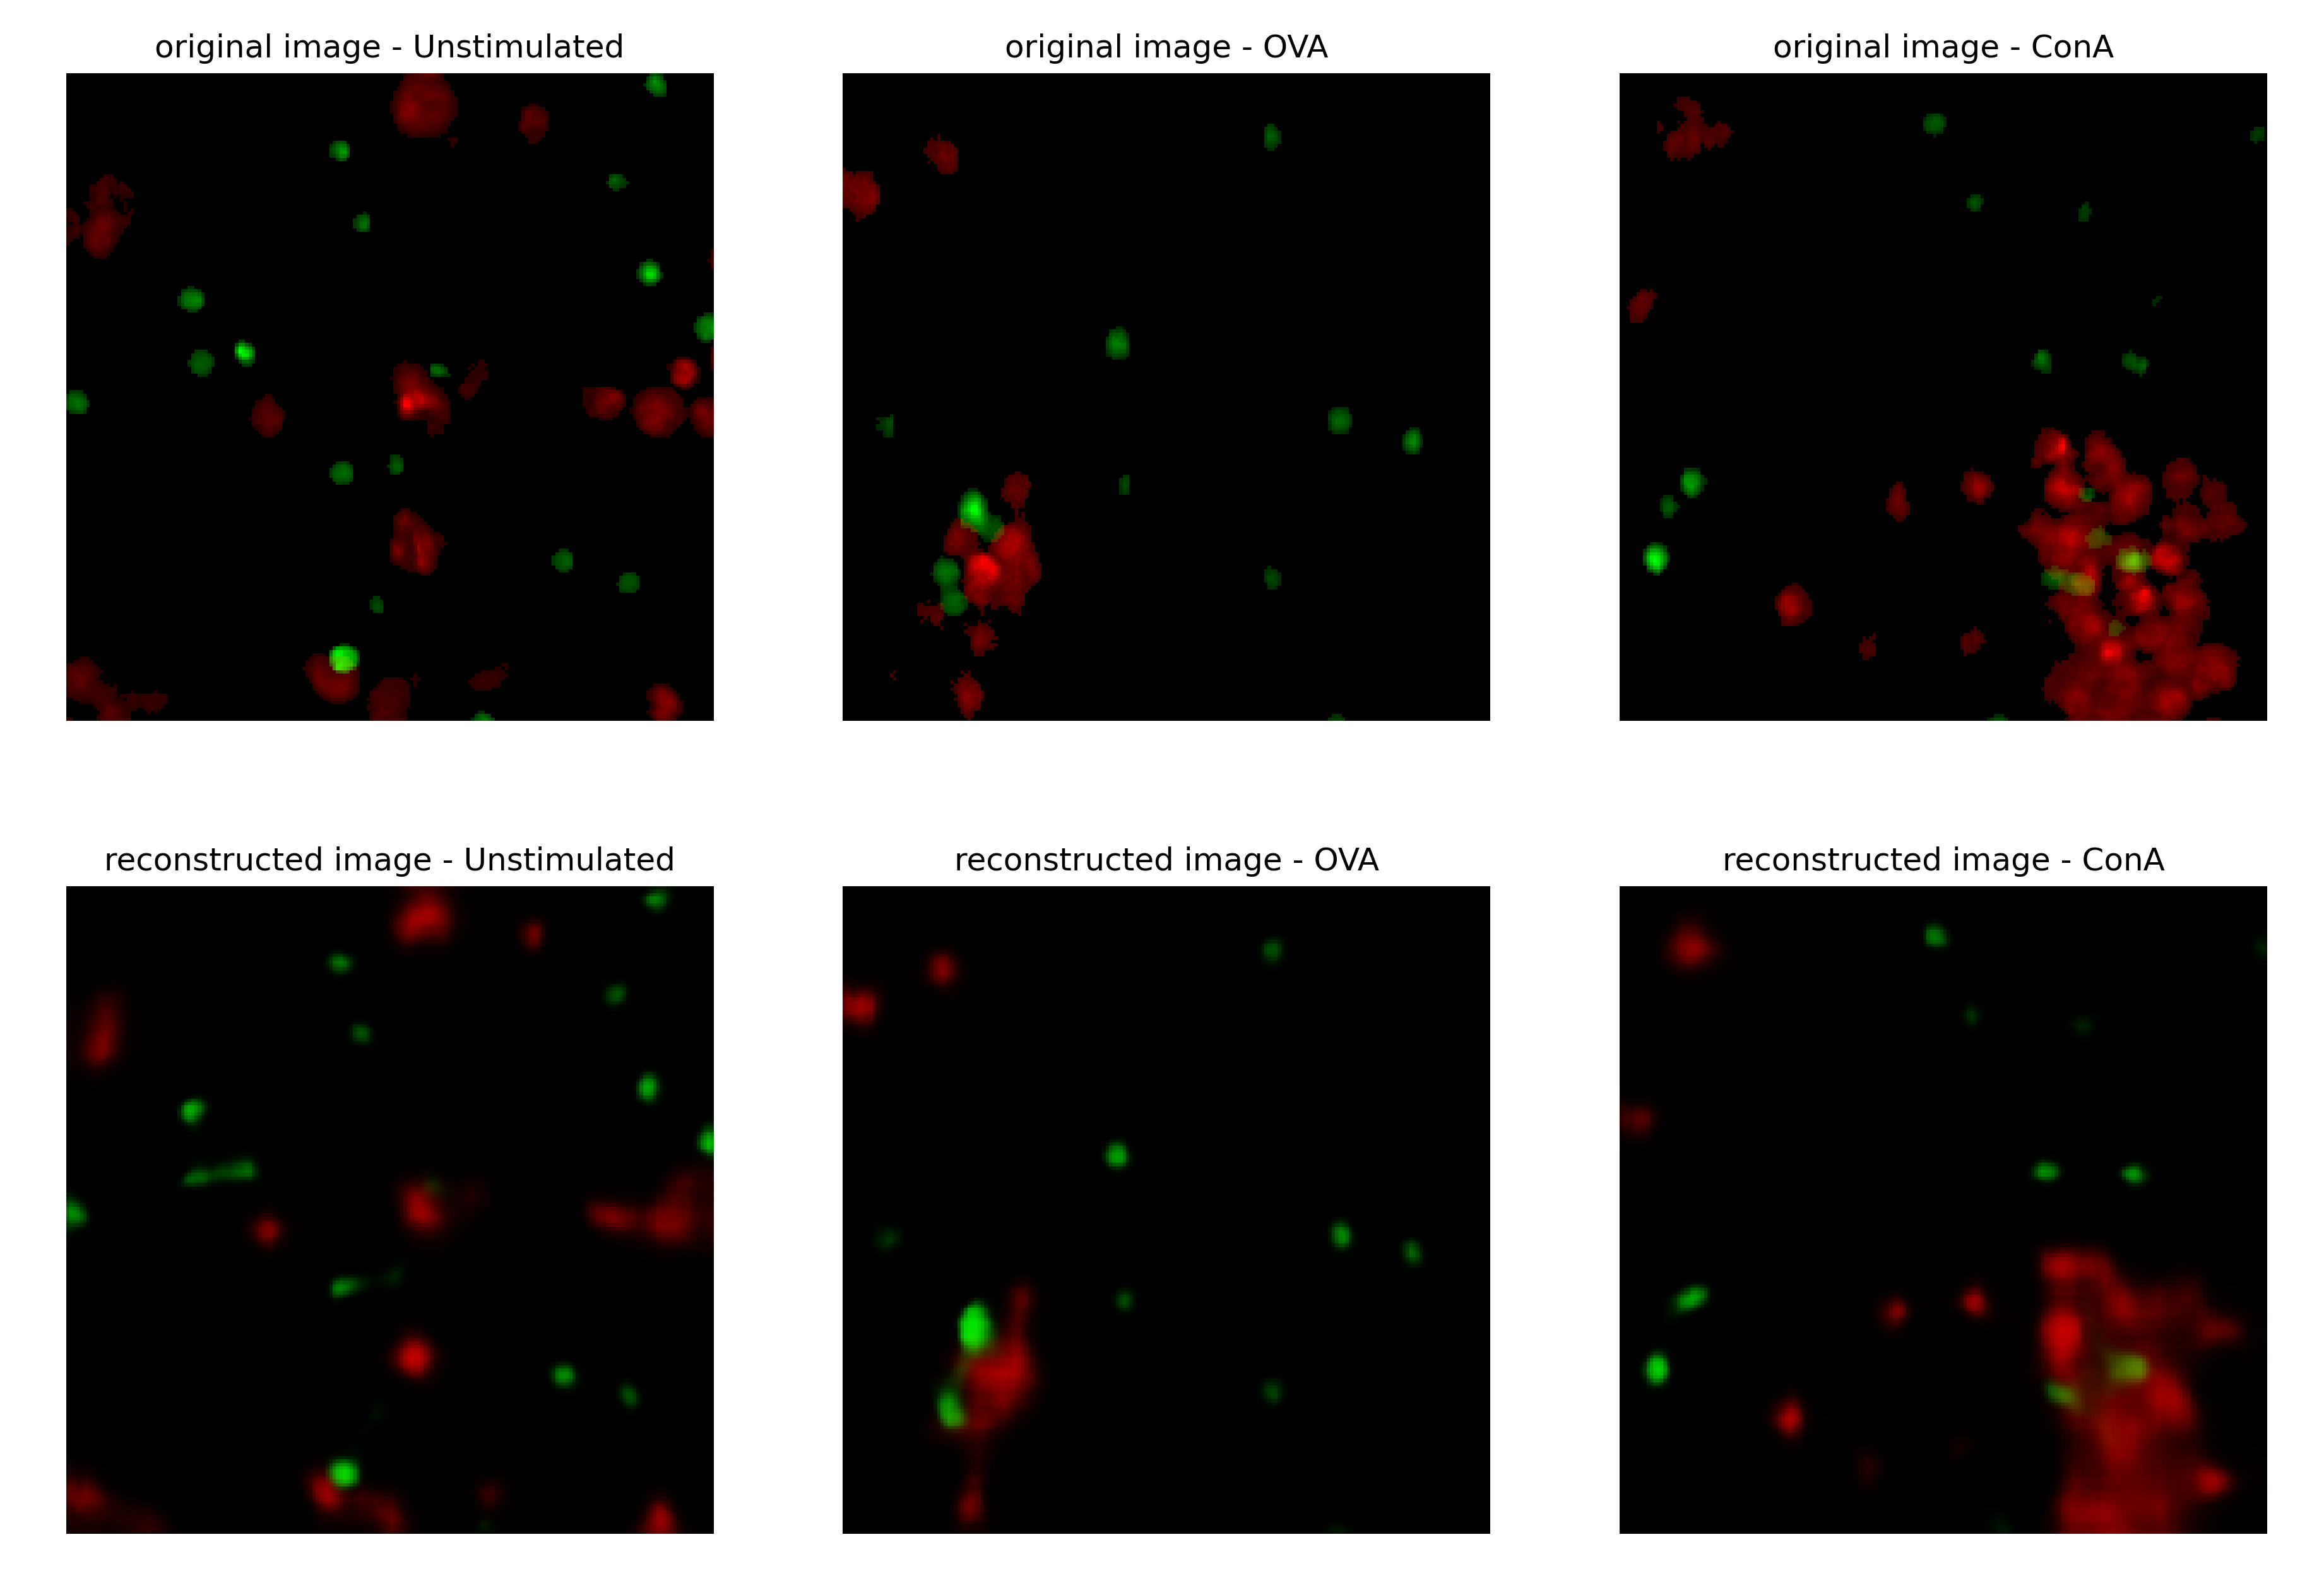
\includegraphics[width=\textwidth]{dissertation/figures/evaluation/CK19_masked_reconstruction.png}
        \caption{Masked images}
    \end{subfigure}
    \caption{Autoencoder-reconstructed images from the test images of \textbf{full} dataset. For each of the subfigures, categories are Unstimulated, OVA, ConA from left to right. Input images are at the top, and reconstructed images at the bottom.}
    \label{fig:full_reconstruction}
\end{figure}

\begin{figure}[h!]
    \centering
    \begin{subfigure}[h!]{0.3\textwidth}
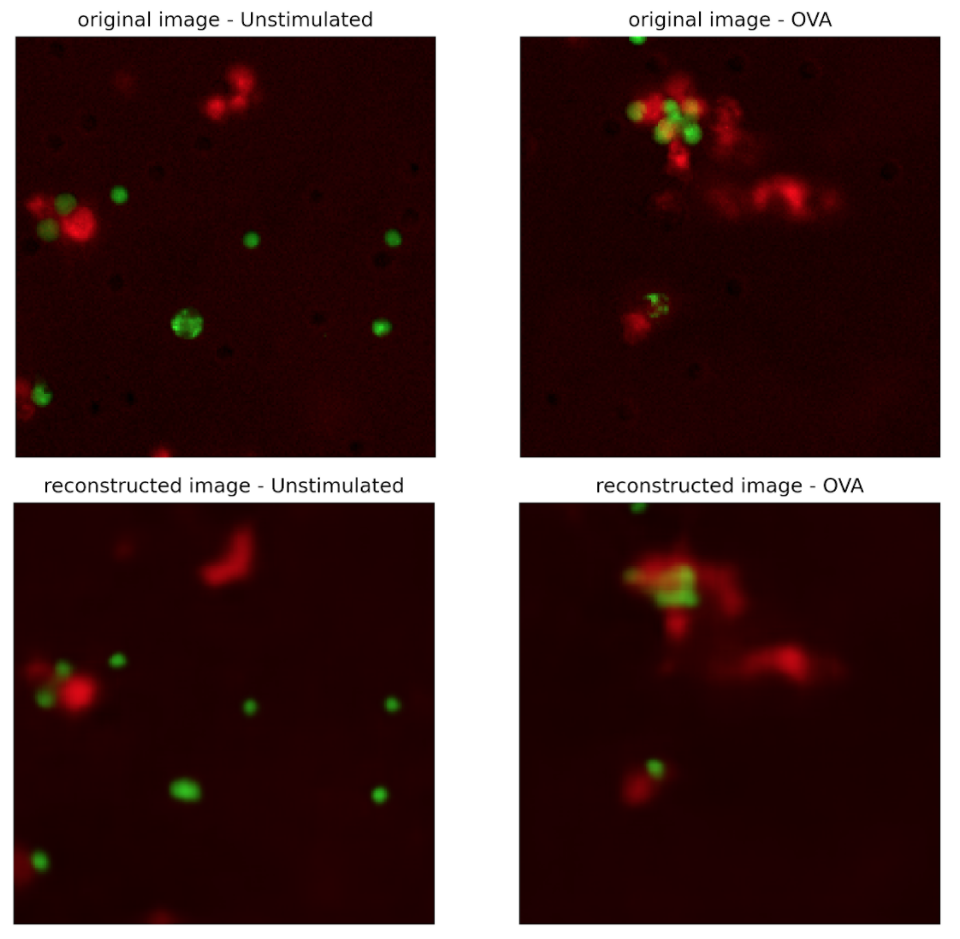
\includegraphics[width=\textwidth]{dissertation/figures/evaluation/CK22_reconstruction.png}
        \caption{Normal images}
    \end{subfigure}
    \begin{subfigure}[h!]{0.3\textwidth}
        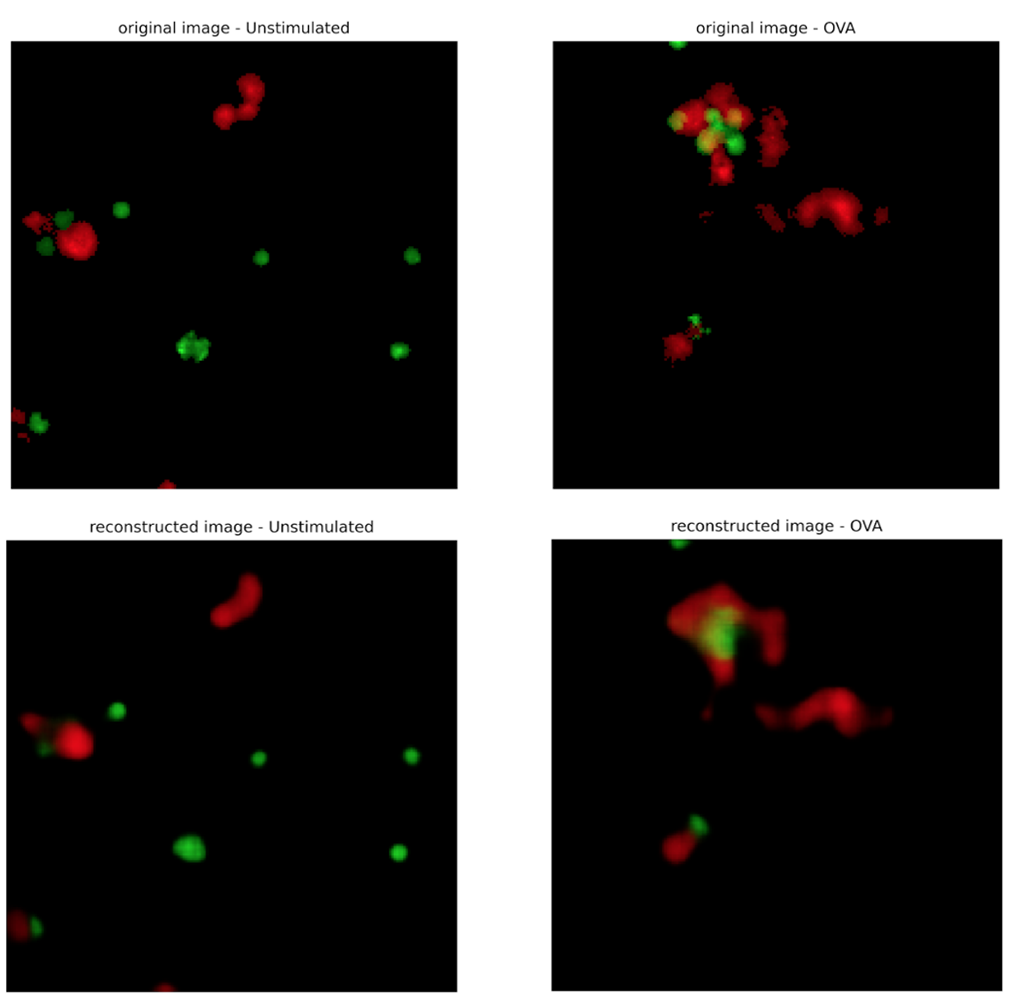
\includegraphics[width=\textwidth]{dissertation/figures/evaluation/CK22_masked_reconstruction.png}
        \caption{Masked images}
        \label{fig:dual_masked_recon}
    \end{subfigure}
    \caption{Autoencoder-reconstructed images from the \textbf{dual} dataset. For each of the subfigures, stimulation categories are Unstimulated (left) and OVA (right). Input images are at the top, and reconstructed images at the bottom.}
    \label{fig:dual_reconstruction}
\end{figure}

\begin{figure}[h!]
    \centering
    \begin{subfigure}[h!]{0.45\textwidth}
        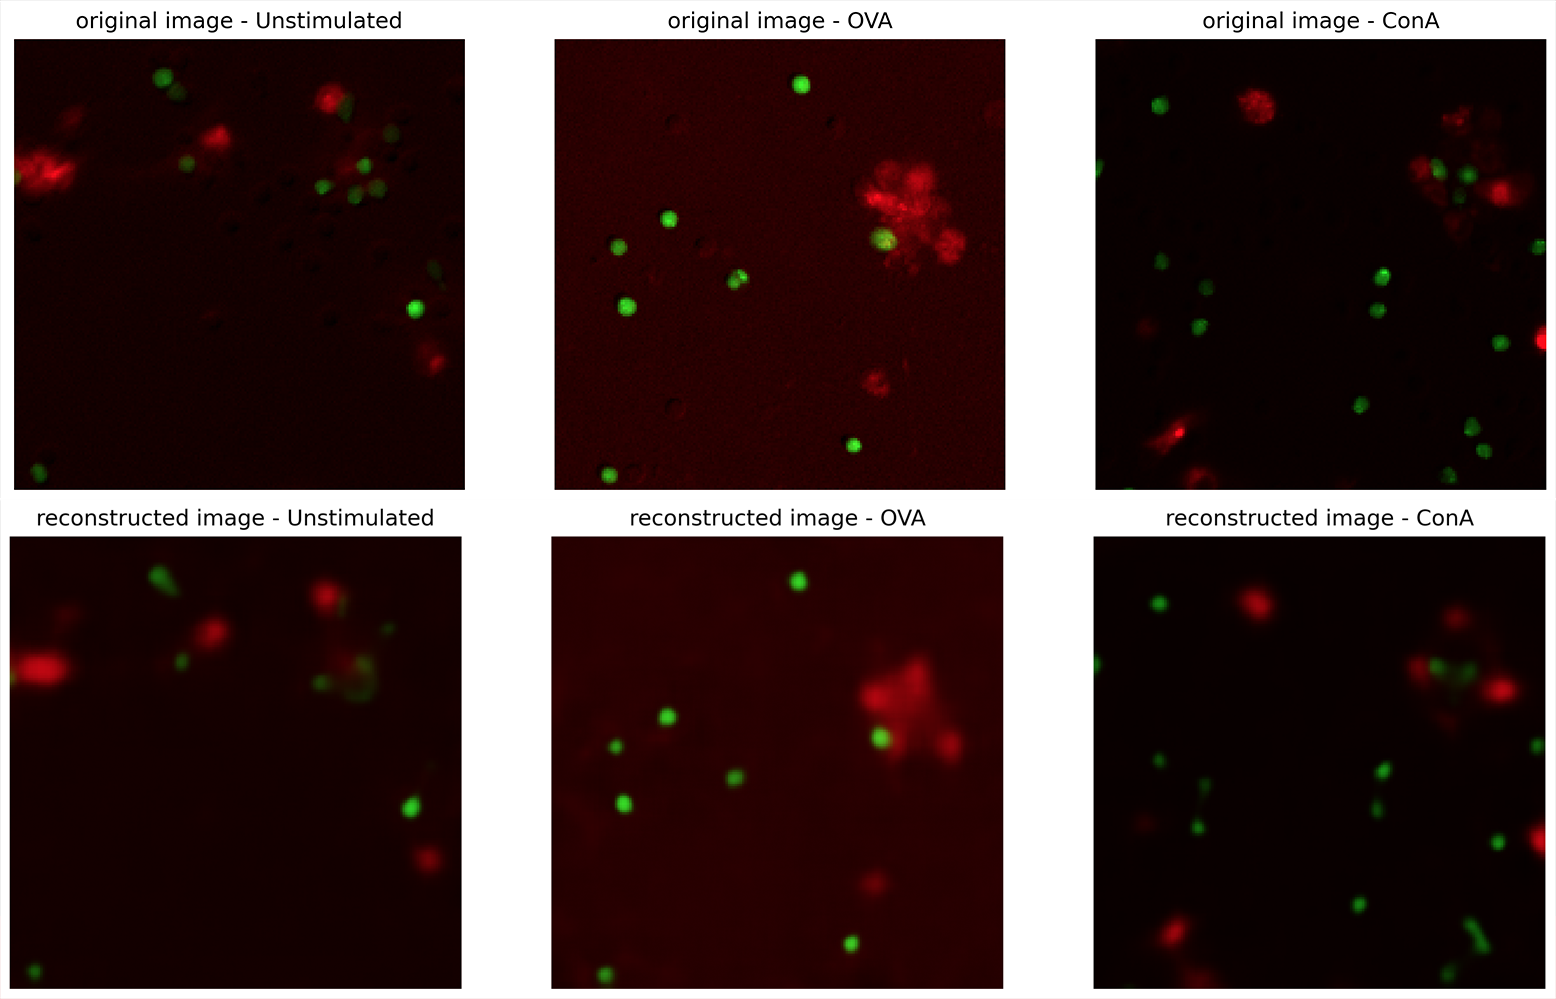
\includegraphics[width=\textwidth]{dissertation/figures/evaluation/DMSO_reconstruction.png}
        \caption{Normal images}
    \end{subfigure}
    %
    \begin{subfigure}[h!]{0.46\textwidth}
        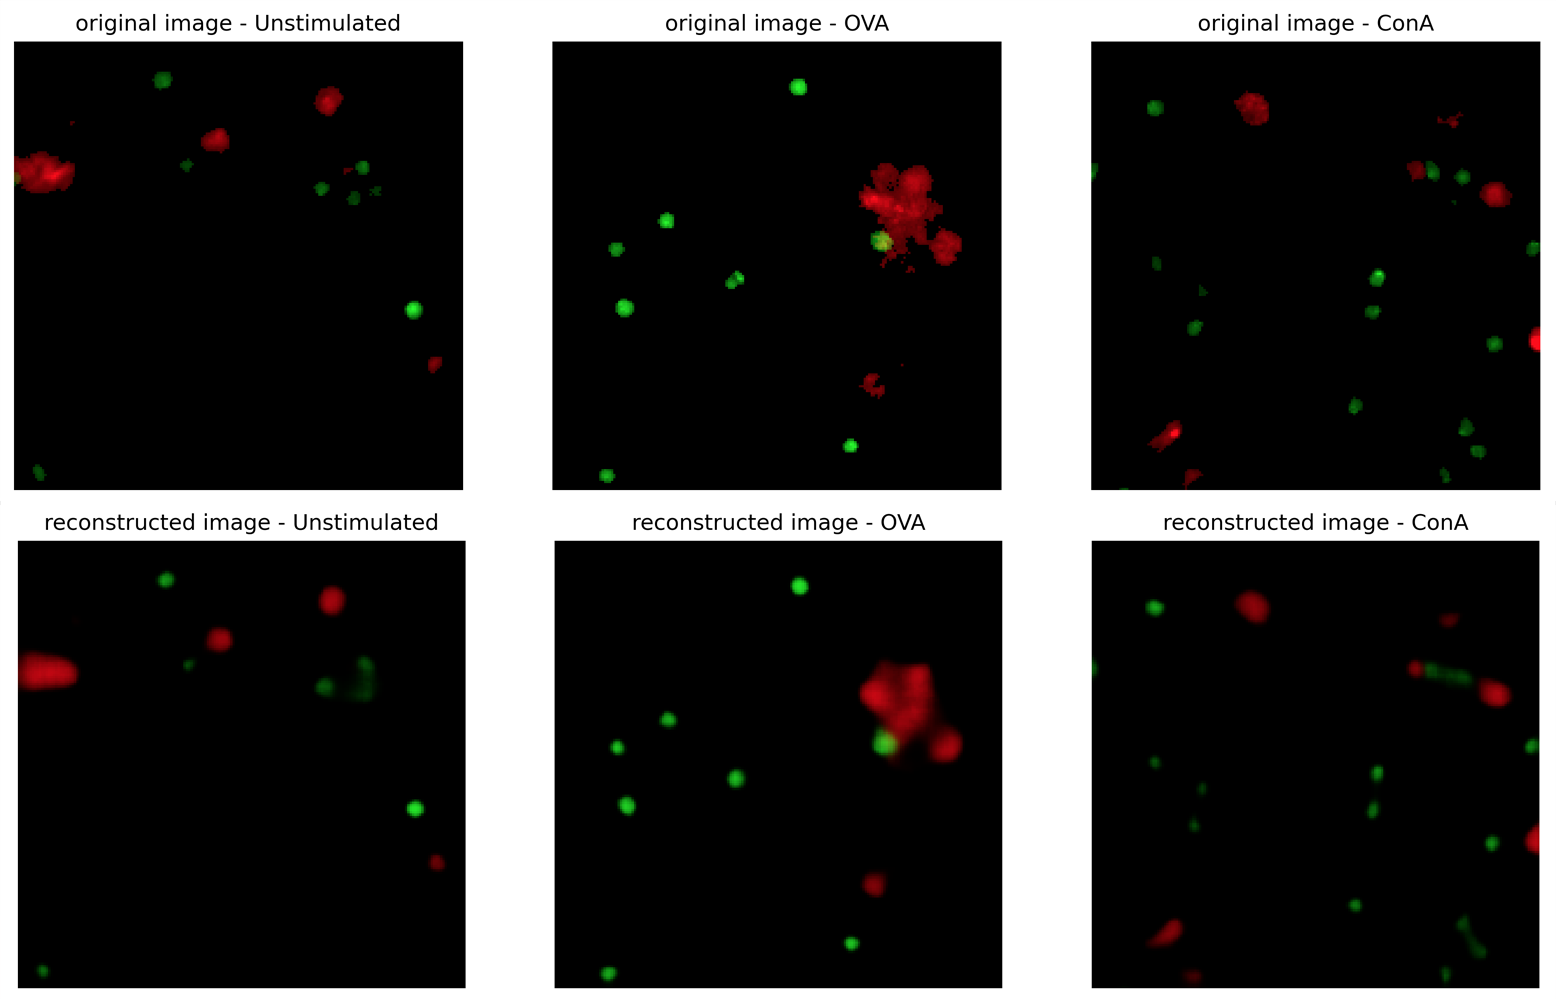
\includegraphics[width=\textwidth]{dissertation/figures/evaluation/DMSO_masked_reconstruction.png}
        \caption{Masked images}
        \label{fig:dmso_masked_recon}
    \end{subfigure}
    \caption{Autoencoder-reconstructed images from the \textbf{DMSO} dataset. For each of the subfigures, categories are Unstimulated, OVA, ConA from left to right. Input images are at the top, and predicted images at the bottom.}
    \label{fig:dmso_reconstruction}
\end{figure}

The main feature we can note from these images is that visually, the autoencoder reconstructed the images in quite a satisfactory way – we can still see where cells are and where they overlap. We can recognise the images's similarities. We can also identify some flaws. The main drawback of the autoencoder model is the way it merges different cells together, creating `blobs' rather than more detailed cell objects.

On the other hand, we can note that the masked autoencoder trained on the masked images of immune cells achieve a higher level of detail, for all datasets. Particularly, the images reconstructed by the masked model retain the circularity of the cell objects better, even in the unseen datasets. This can be observed in Figures \ref{fig:dual_masked_recon} and \ref{fig:dmso_masked_recon} where the dendritic cells in red hold their original shape and detail better in comparison to their non-masked counterpart.

Visually, it is not immediately clear how much better the autoencoder performs on the full dataset, part of which it has seen, compared to the unseen dual and DMSO datasets. Indeed, we will not be able to fully compare the reconstruction of these images by eye. Further to visual evaluation of the reconstruction of the immune cells, the two models's prediction losses can provide another perspective on their performance. Table \ref{tab:autoencoder_loss} reports loss values for each model on each dataset.

\begin{table}[!h]
\centering
\caption{Binary cross-entropy loss value for the autoencoder models's performances on each of the test datasets. A value closer to 0 is better. We can observe a gain in performance across datasets in the masked model.}
\label{tab:autoencoder_loss}
\begin{tabular}{l|r|r|r}
\rowcolor[HTML]{EFEFEF} 
Model  & Full   & Dual   & DMSO   \\ \hline
Normal & 0.0870 & 0.1159 & 0.0936 \\ \hline
Masked & 0.0156 & 0.0174 & 0.0166 \\
\end{tabular}
\end{table}

From this data we can say that removing noisy backgrounds entirely from the images of immune cells achieved substantial improvements. It also made the autoencoder's performance on unseen datasets more comparable to the full dataset.

\subsection{Can we find an underlying structure in the images of immune cells?}

While we have shown that an autoencoder can complete the task of reducing the dimensionality of an image of immune cells and reconstruct it fully from this reduced image, we want to look at whether or not this would help with a two-dimensional projection of the datasets. The aim for two-dimensional visualisation of the datasets was that it would allow us to uncover clusters of images grouped around the same stimulation conditions.

Each element projected onto a 2D plane is labelled with one of the \textit{Unstimulated}, \textit{OVA}, \textit{ConA}, or \textit{Faulty} categories at the plotting step.

\bigskip
\subsubsection{Baseline performance}
\hfill
\hfill 

The expectations were that an autoencoder would allow us to extract the necessary features from an image that would be sufficient for it to be reconstructed, but also for it to be analysed. As such, we wanted to compare the visualisation performance of UMAP on the coded images to a baseline performance on raw images that have not been reduced in dimensionality. This was only ran for the full dataset as the large dimensions meant this computation took a considerable amount of time. On a 2015 MacBook Pro with 2.7 GHz i5 core and 8 GB of RAM, running UMAP on the $10,000\times192\times192\times3$ test instances of the full dataset worth took 1 hour, 5 minutes and 33 seconds. The result visualisation is shown in Figure \ref{fig:baseline_vis}.


\begin{figure}[h!]
    \centering
    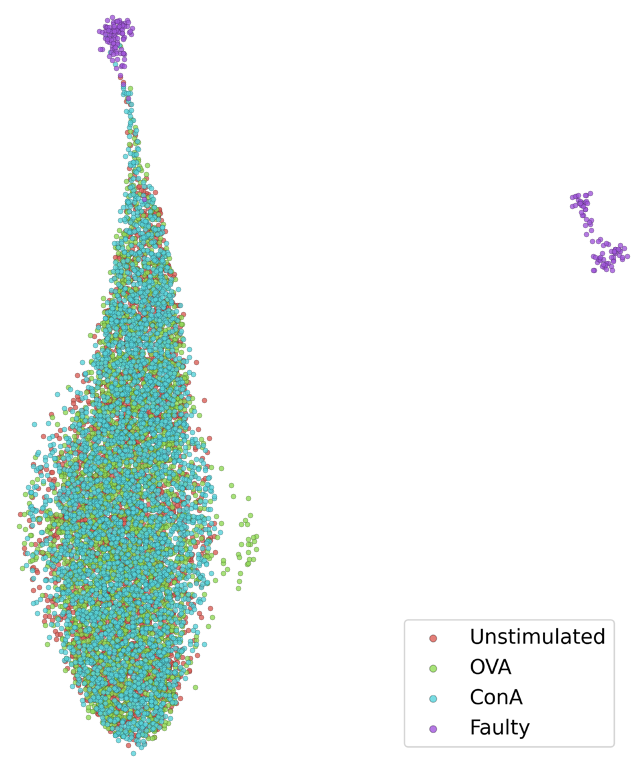
\includegraphics[width=0.45\textwidth]{dissertation/figures/evaluation/CK19_baseline_visualisation.png}
    \caption{Two-dimensional UMAP projection of the 10,000 testing images in the full dataset. UMAP was ran with base parameters $n\_neighbors=15$, $min\_dist=0.1$. The legend highlights which colour corresponds to which stimulation category.}
    \label{fig:baseline_vis}
\end{figure}

This projection highlights that with the raw $192\times193\times3$ images of immune cells, only \textit{Faulty} images seem to be recognised and there is no clear distinction between images of other categories. A few OVA/green points are distanced from the main cluster. We will now look at whether reducing the dimensionality of the images with an autoencoder helps make this distinction.  

\bigskip
\subsubsection{Trained performance}
\hfill
\hfill 

UMAP's speed allowed us to try different parameters for our visualisations to attempt to yield the best projections of the data, as running UMAP only took between 30 seconds and 1 minute and 15 seconds to run on the encoder-processed images. That is an average 75x speedup on the baseline performance.

We can see the projection of the \textbf{full dataset}'s test images in Figure \ref{fig:full_reconstruction}. Two smaller clusters have emerged which were not present in the baseline projection. The labelling shows us that the sparser cluster contains two lines of red/Unstimulated and green/ConA points, which could indicate that the autoencoder did help extract the most important features out of the images. However, the larger cluster still bears no distinction between images of different categories. Furthermore, the projection obtained with the masked model did not seem to perform better, with less clusters being uncovered this way.

\begin{figure}[h!]
    \centering
    \begin{subfigure}[h!]{0.39\textwidth}
        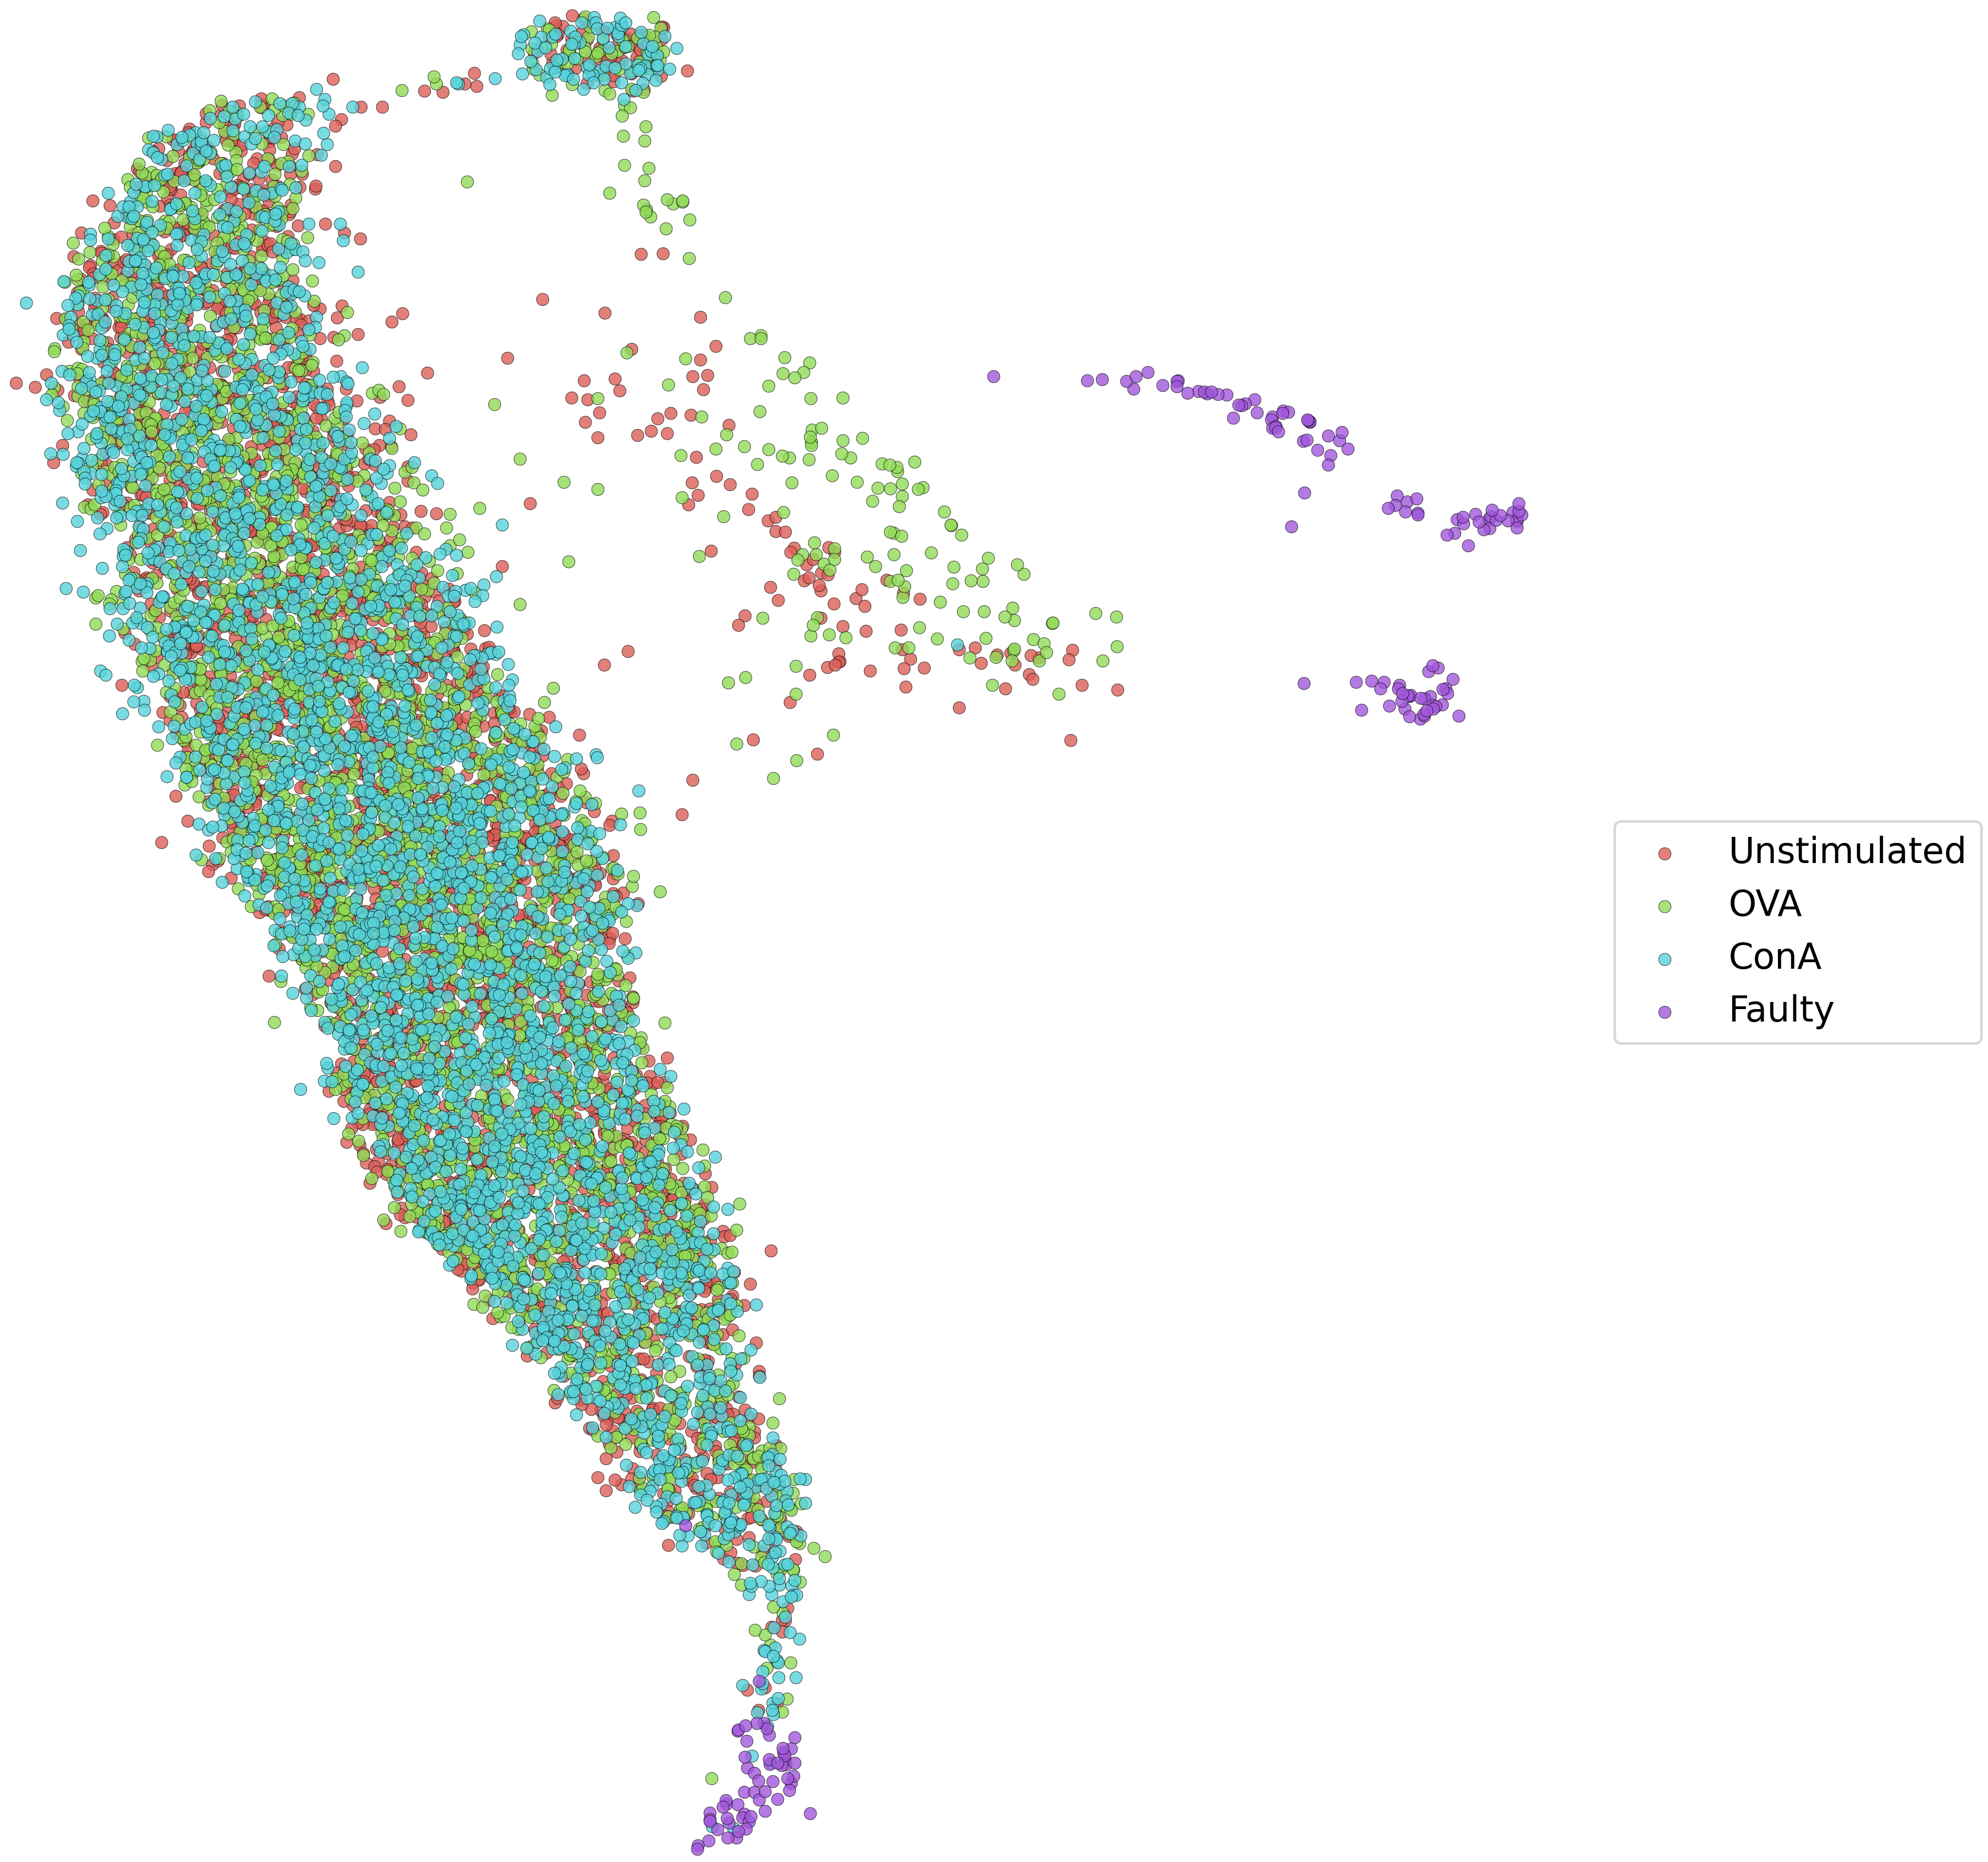
\includegraphics[width=\textwidth]{dissertation/figures/evaluation/CK19_umap.png}
        \caption{Normal images}
        \label{subfig:full_projection_normal}
    \end{subfigure}
    \begin{subfigure}[h!]{0.41\textwidth}
        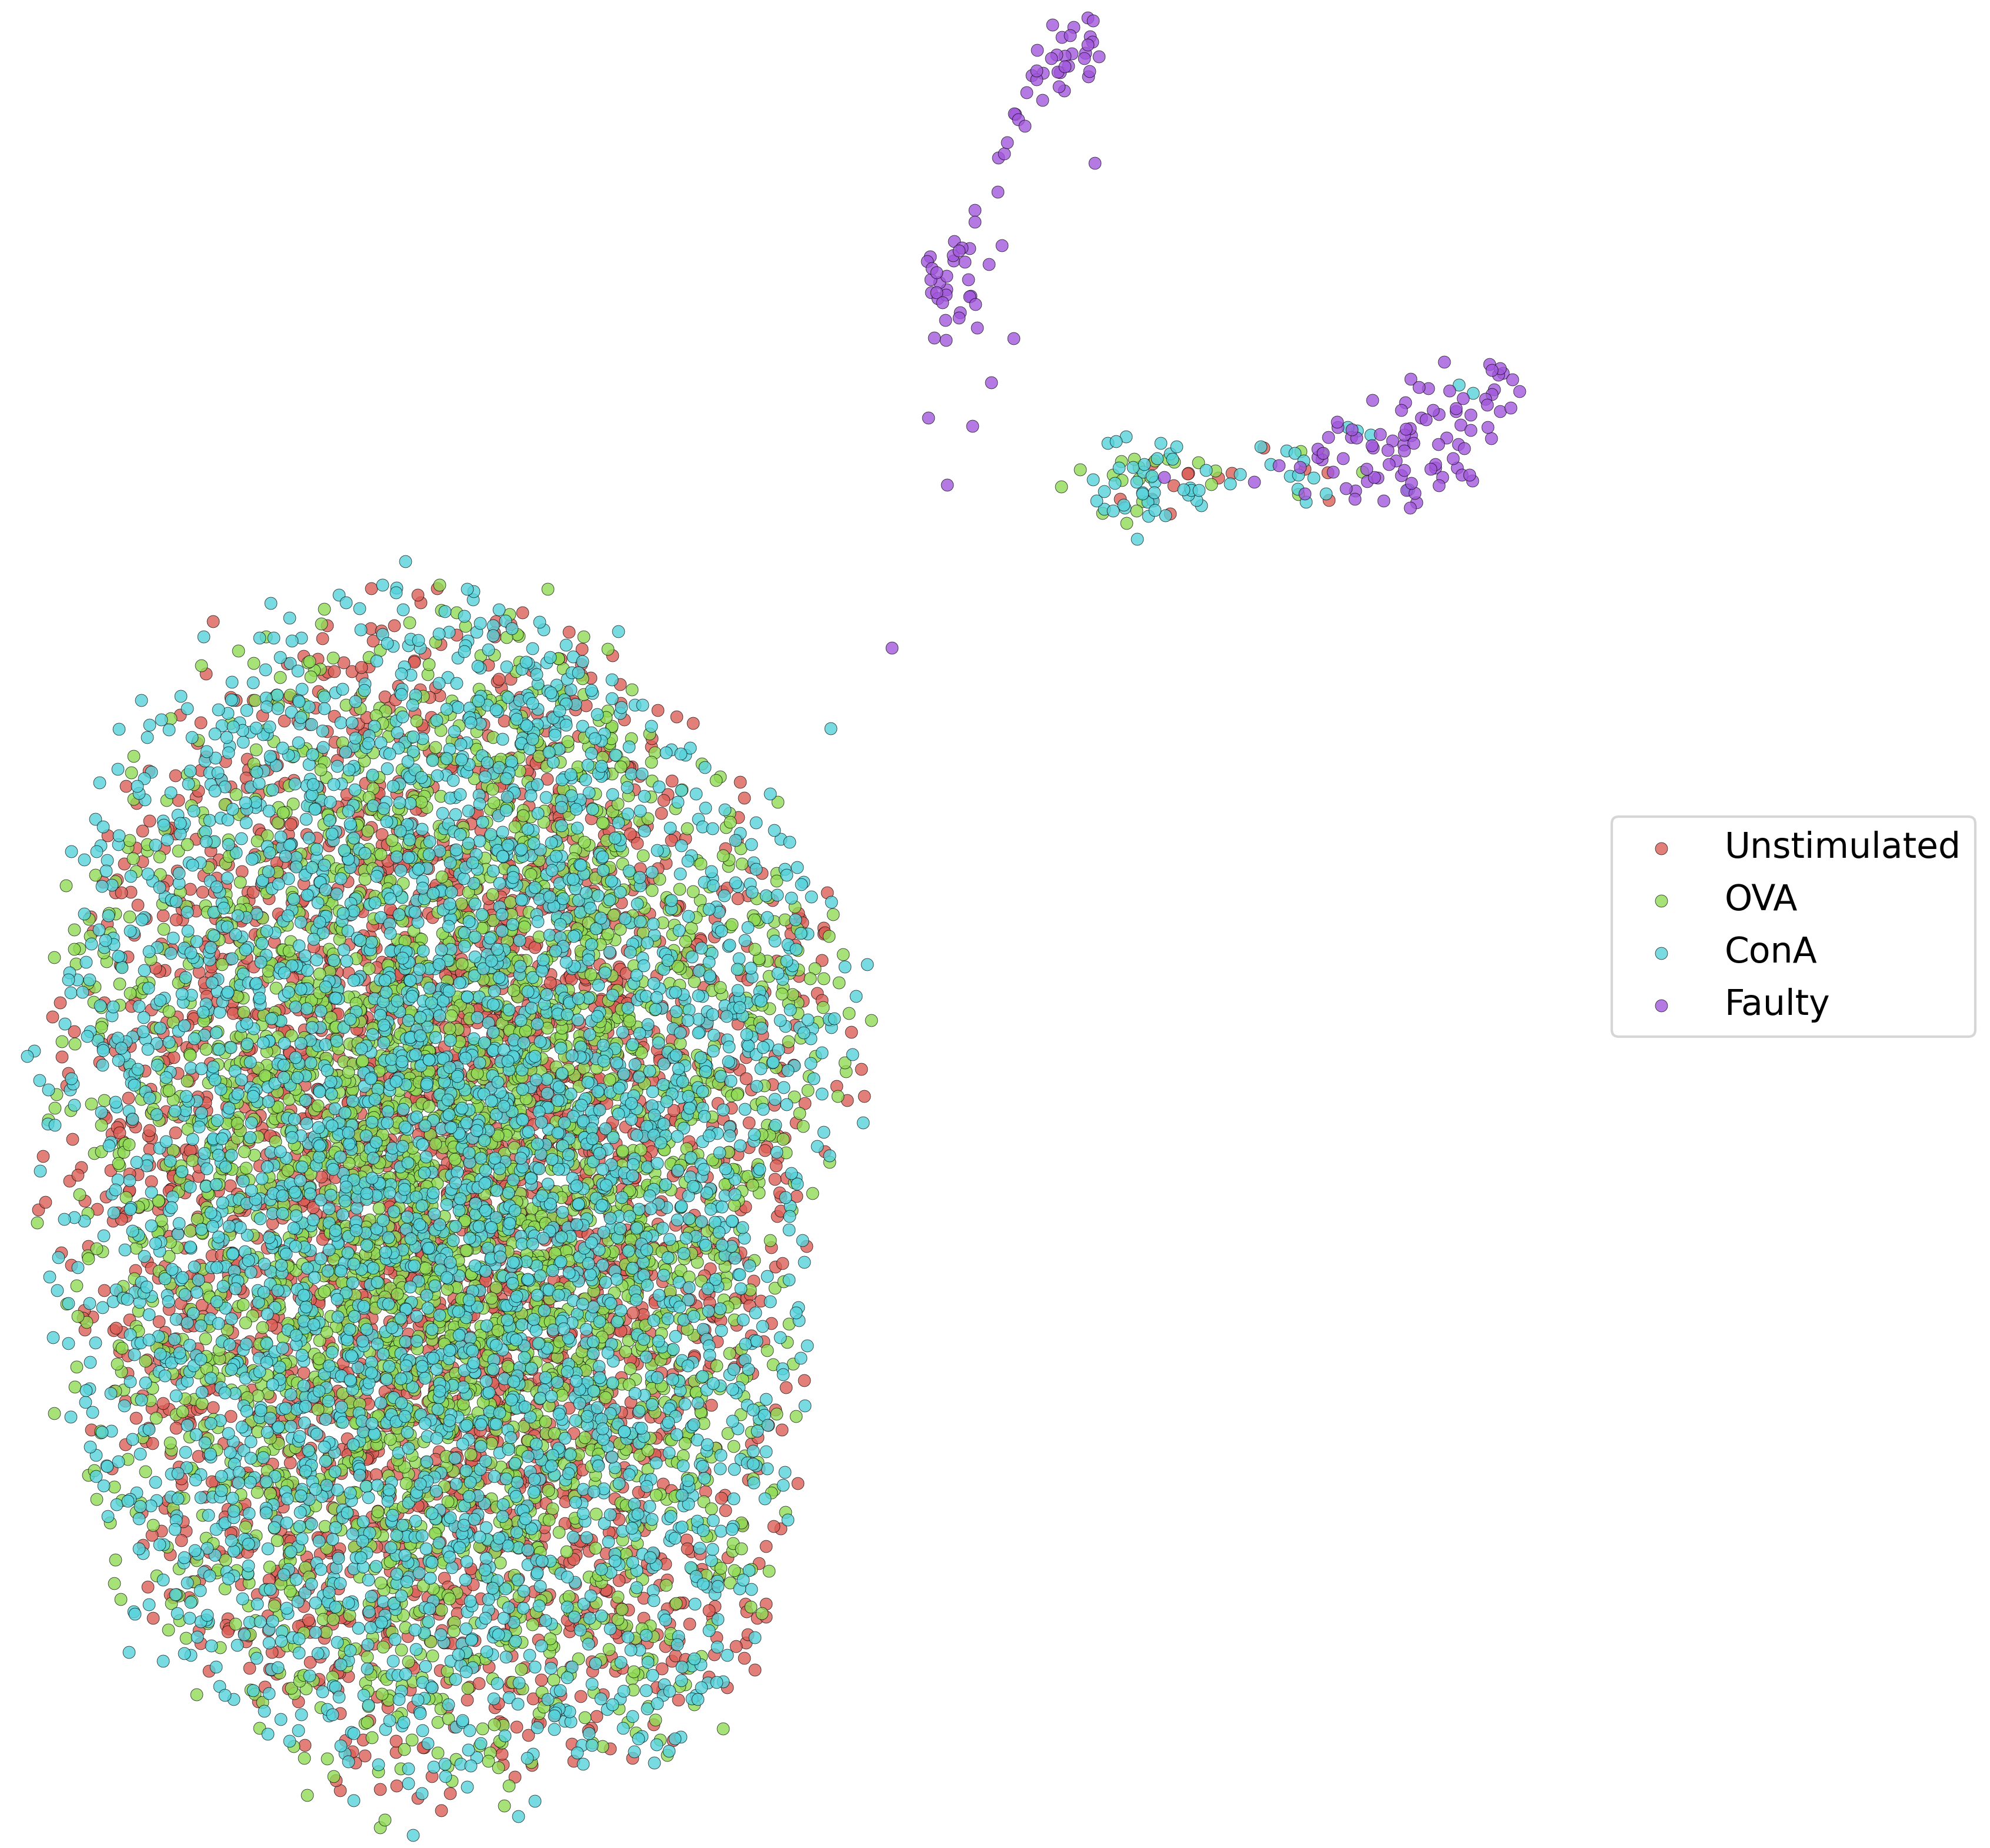
\includegraphics[width=\textwidth]{dissertation/figures/evaluation/CK19_masked_umap.png}
        \caption{Masked images}
    \end{subfigure}
    \caption{Two-dimensional UMAP projections of the 10,000 test images from the \textbf{full} dataset. These projection were obtained with UMAP parameters n\_neighbors=30 and min\_dist=0.8. The legend highlights which colour corresponds to which stimulation category.}
    \label{fig:full_projection}
\end{figure}

We hoped for the \textbf{dual dataset} to perform better as it only had two stimulation categories to distinguish between. The normal and masked visualisations are shown in Figure \ref{fig:dual_visualisation}. Although no clear distinction of clusters is shown the normal projection, a small cluster formed in the projection of the masked dataset. However, this cluster contains images of both \textit{Unstimulated} and \textit{OVA} categories. 

\begin{figure}[ht!]
    \centering
    \begin{subfigure}[ht]{0.35\textwidth}
        \includegraphics[width=\textwidth]{dissertation/figures/evaluation/CK22_umap.png}
        \caption{Normal images}
    \end{subfigure}
    \begin{subfigure}[ht]{0.35\textwidth}
        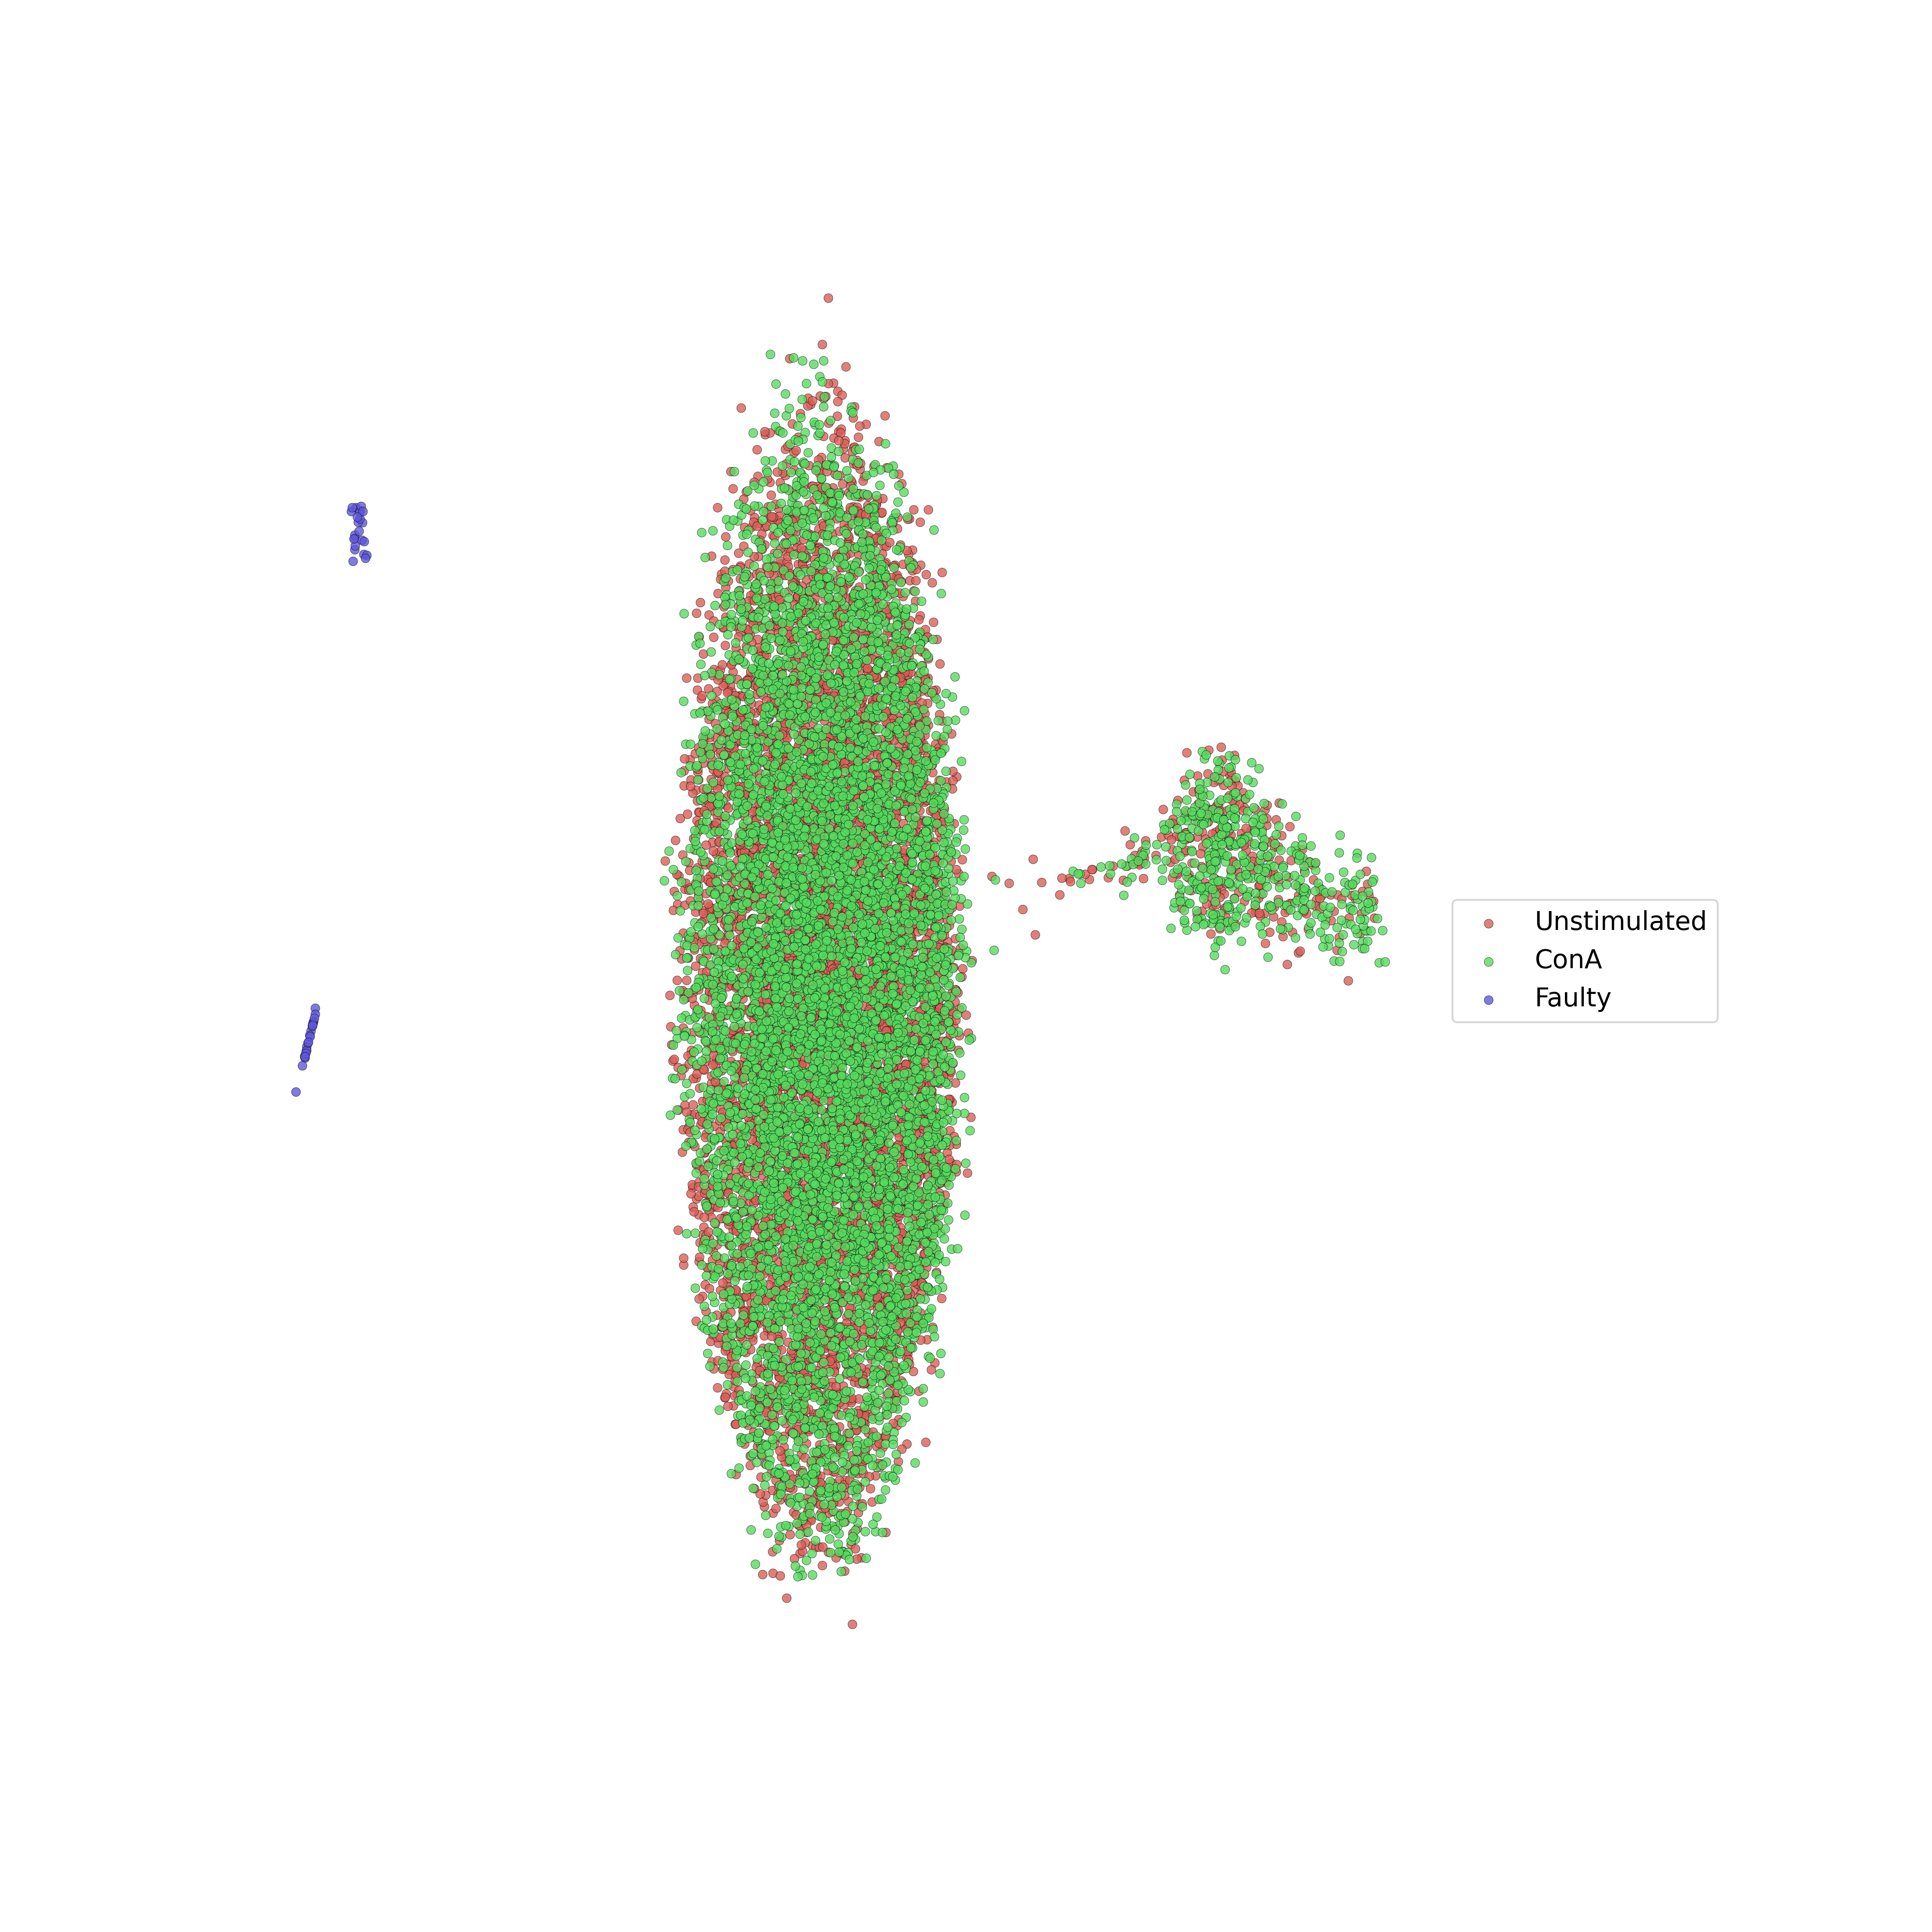
\includegraphics[width=\textwidth]{dissertation/figures/evaluation/CK22_masked_umap.png}
        \caption{Masked images}
        \label{subfig:dual_projection_masked}
    \end{subfigure}
    \caption{Two-dimensional UMAP projection of the 13,800 test images from the \textbf{dual} dataset. These projections were obtained with UMAP parameters n\_neighbors=30 and min\_dist=0.8. The legend highlights which colour corresponds to which stimulation category. The normal images are not clearly distinguished by category, but the masked images yield a separate cluster. None of these clusters bear distinction between images of different stimulation.}
    \label{fig:dual_visualisation}
\end{figure}

The images from the DMSO images should show the most distinction between each other as the immune cells from the images have only been influenced by the stimulation antigens and no other compounds, while immune cells from the experiments represented in the other two datasets have also been injected with drug compounds.

The \textbf{DMSO} projection is shown in Figure \ref{fig:dmso_projection}, from which we can observe some interesting features. Firstly, there is one main cluster, but interestingly the coloured points show a green to blue gradient, which we could attribute to a distinction between the \textit{OVA} and \textit{ConA} categories. Blue/\textit{ConA} points become sparser at the top of the cluster, and the same happens for green/\textit{OVA} points at the bottom of the cluster. This is overlaid on top of images of the \textit{Unstimulated} category, however this might show that some distinction is being made between the images. Furthermore, we can see two smaller collections of red/\textit{Unstimulated} points and green/\textit{OVA} points. The projection of masked images does not show this \textit{OVA-ConA} distinction, but does have a separate cluster of \textit{Unstimulated/OVA} points.

\begin{figure}[h!]
    \centering
    \begin{subfigure}[h!]{0.4\textwidth}
        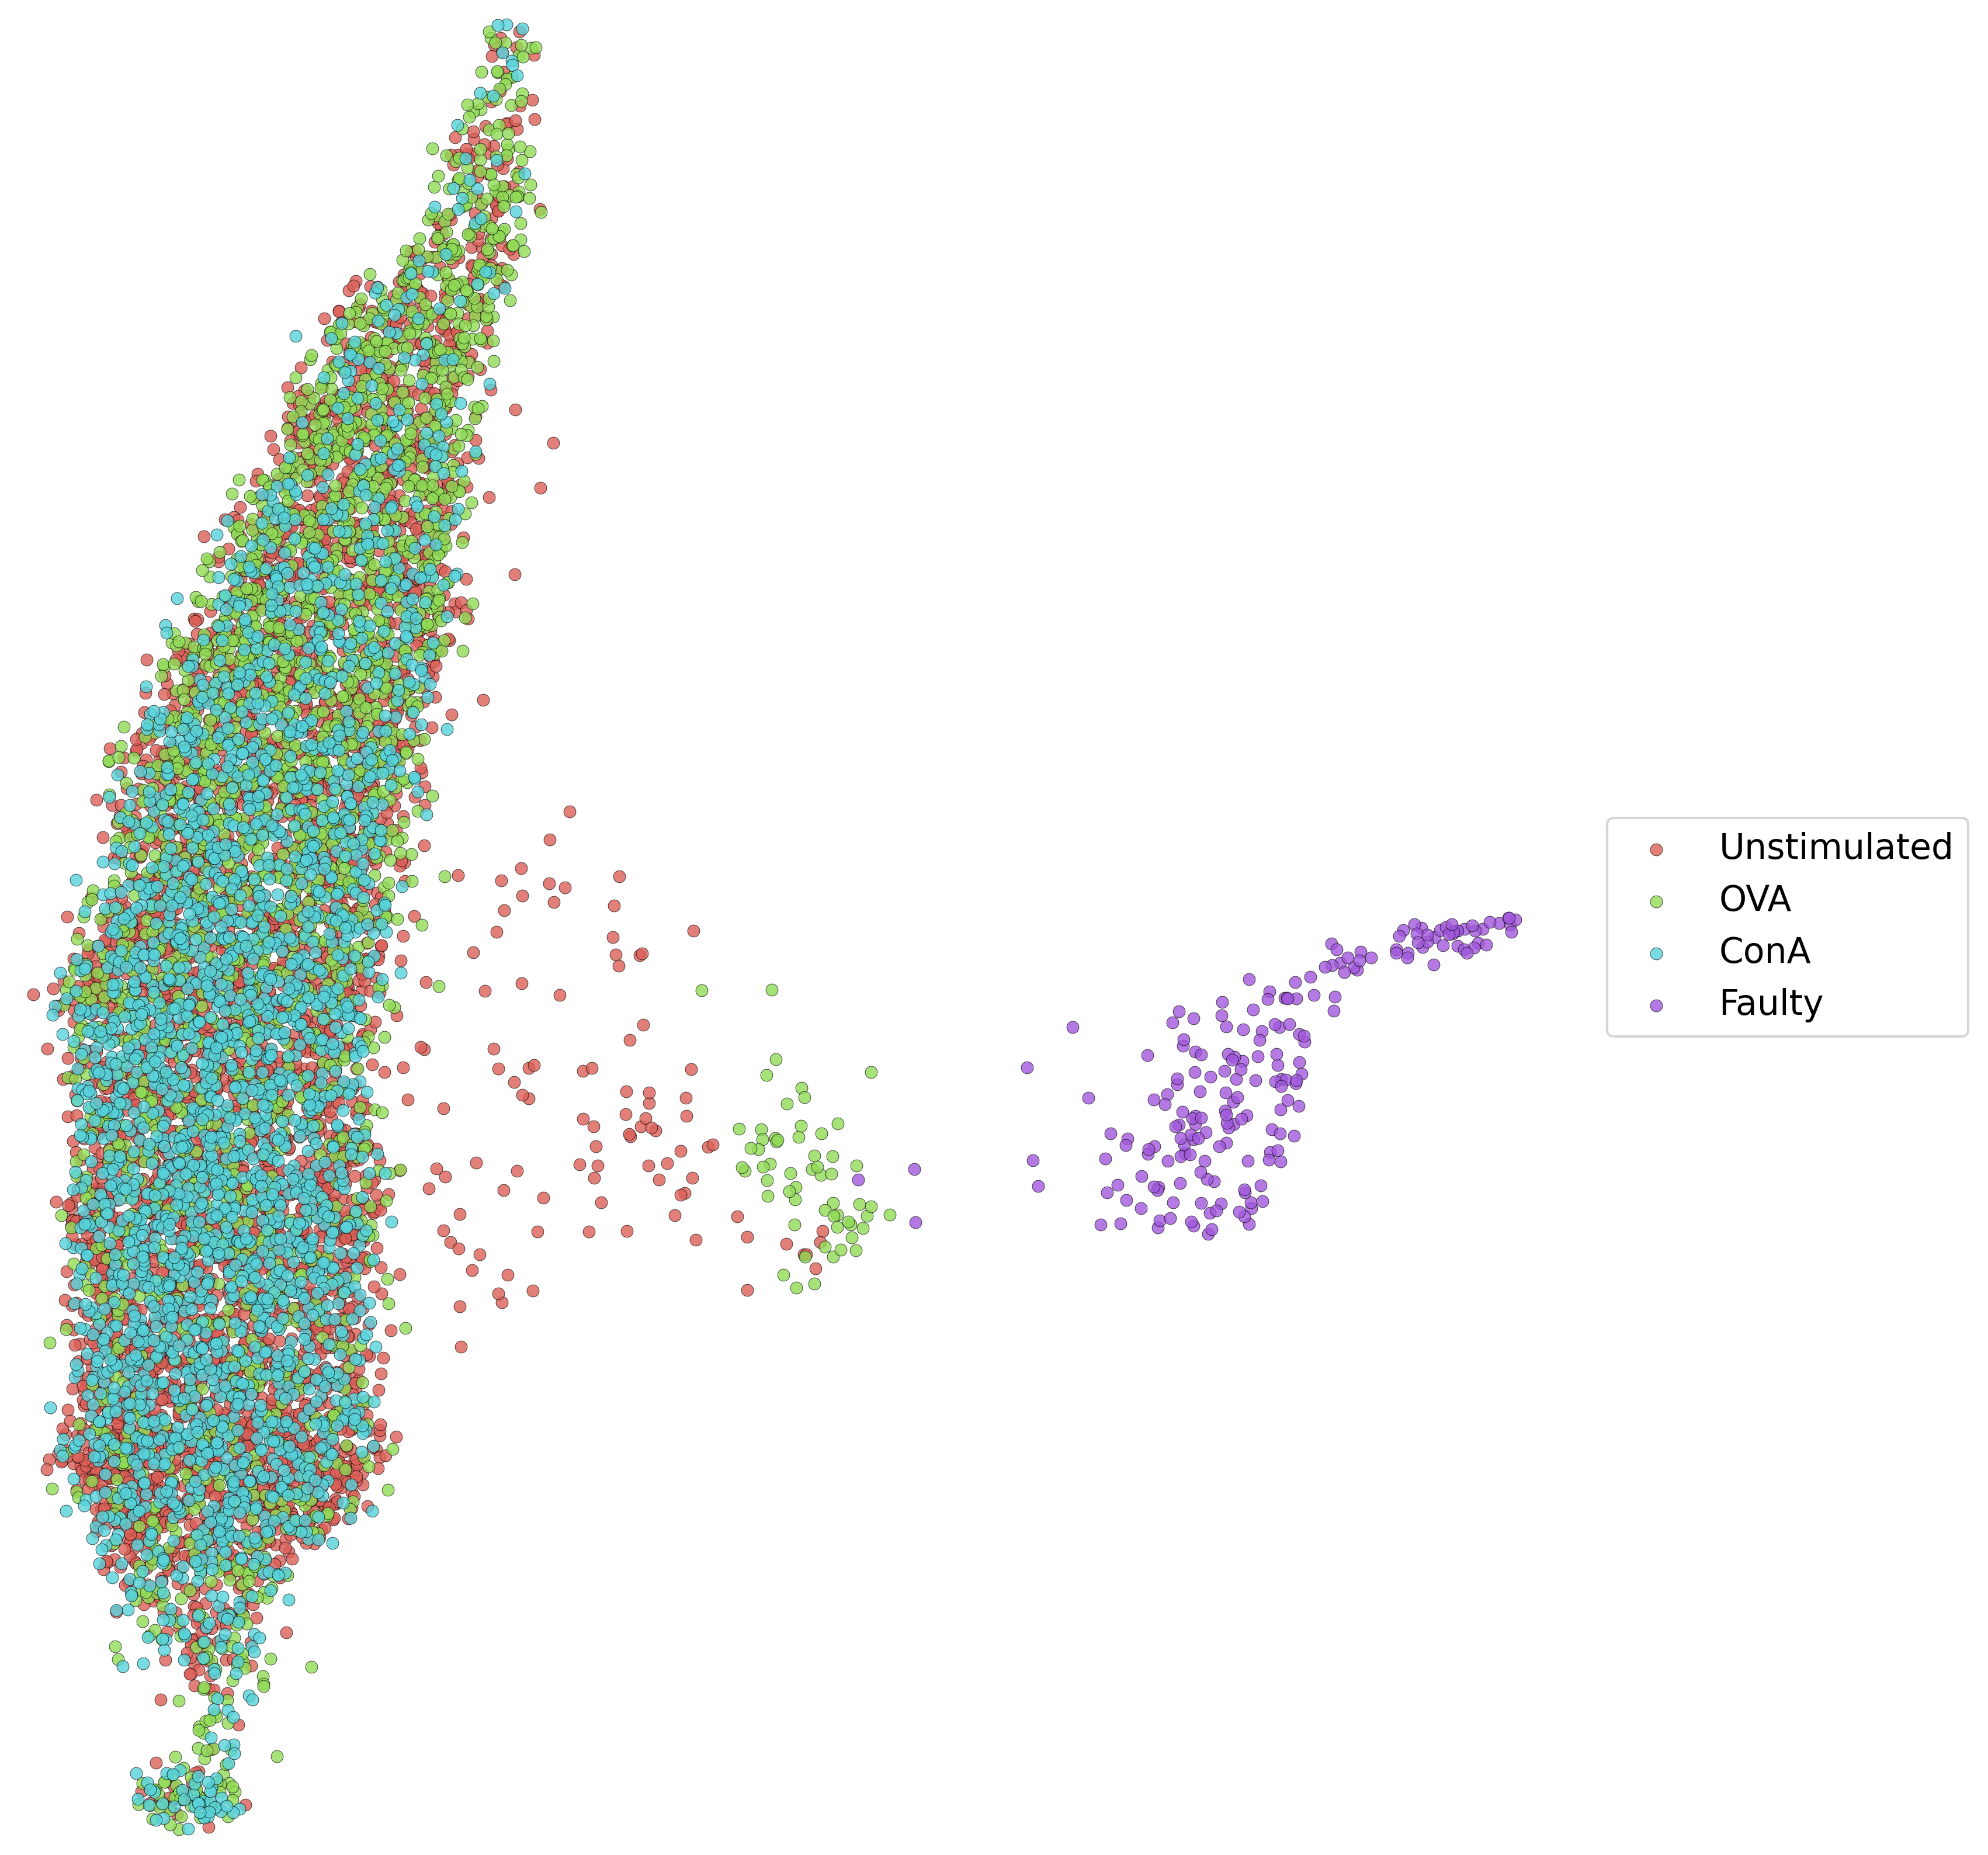
\includegraphics[width=\textwidth]{dissertation/figures/evaluation/DMSO_umap.png}
        \caption{Normal images}
    \end{subfigure}
    \begin{subfigure}[h!]{0.4\textwidth}
        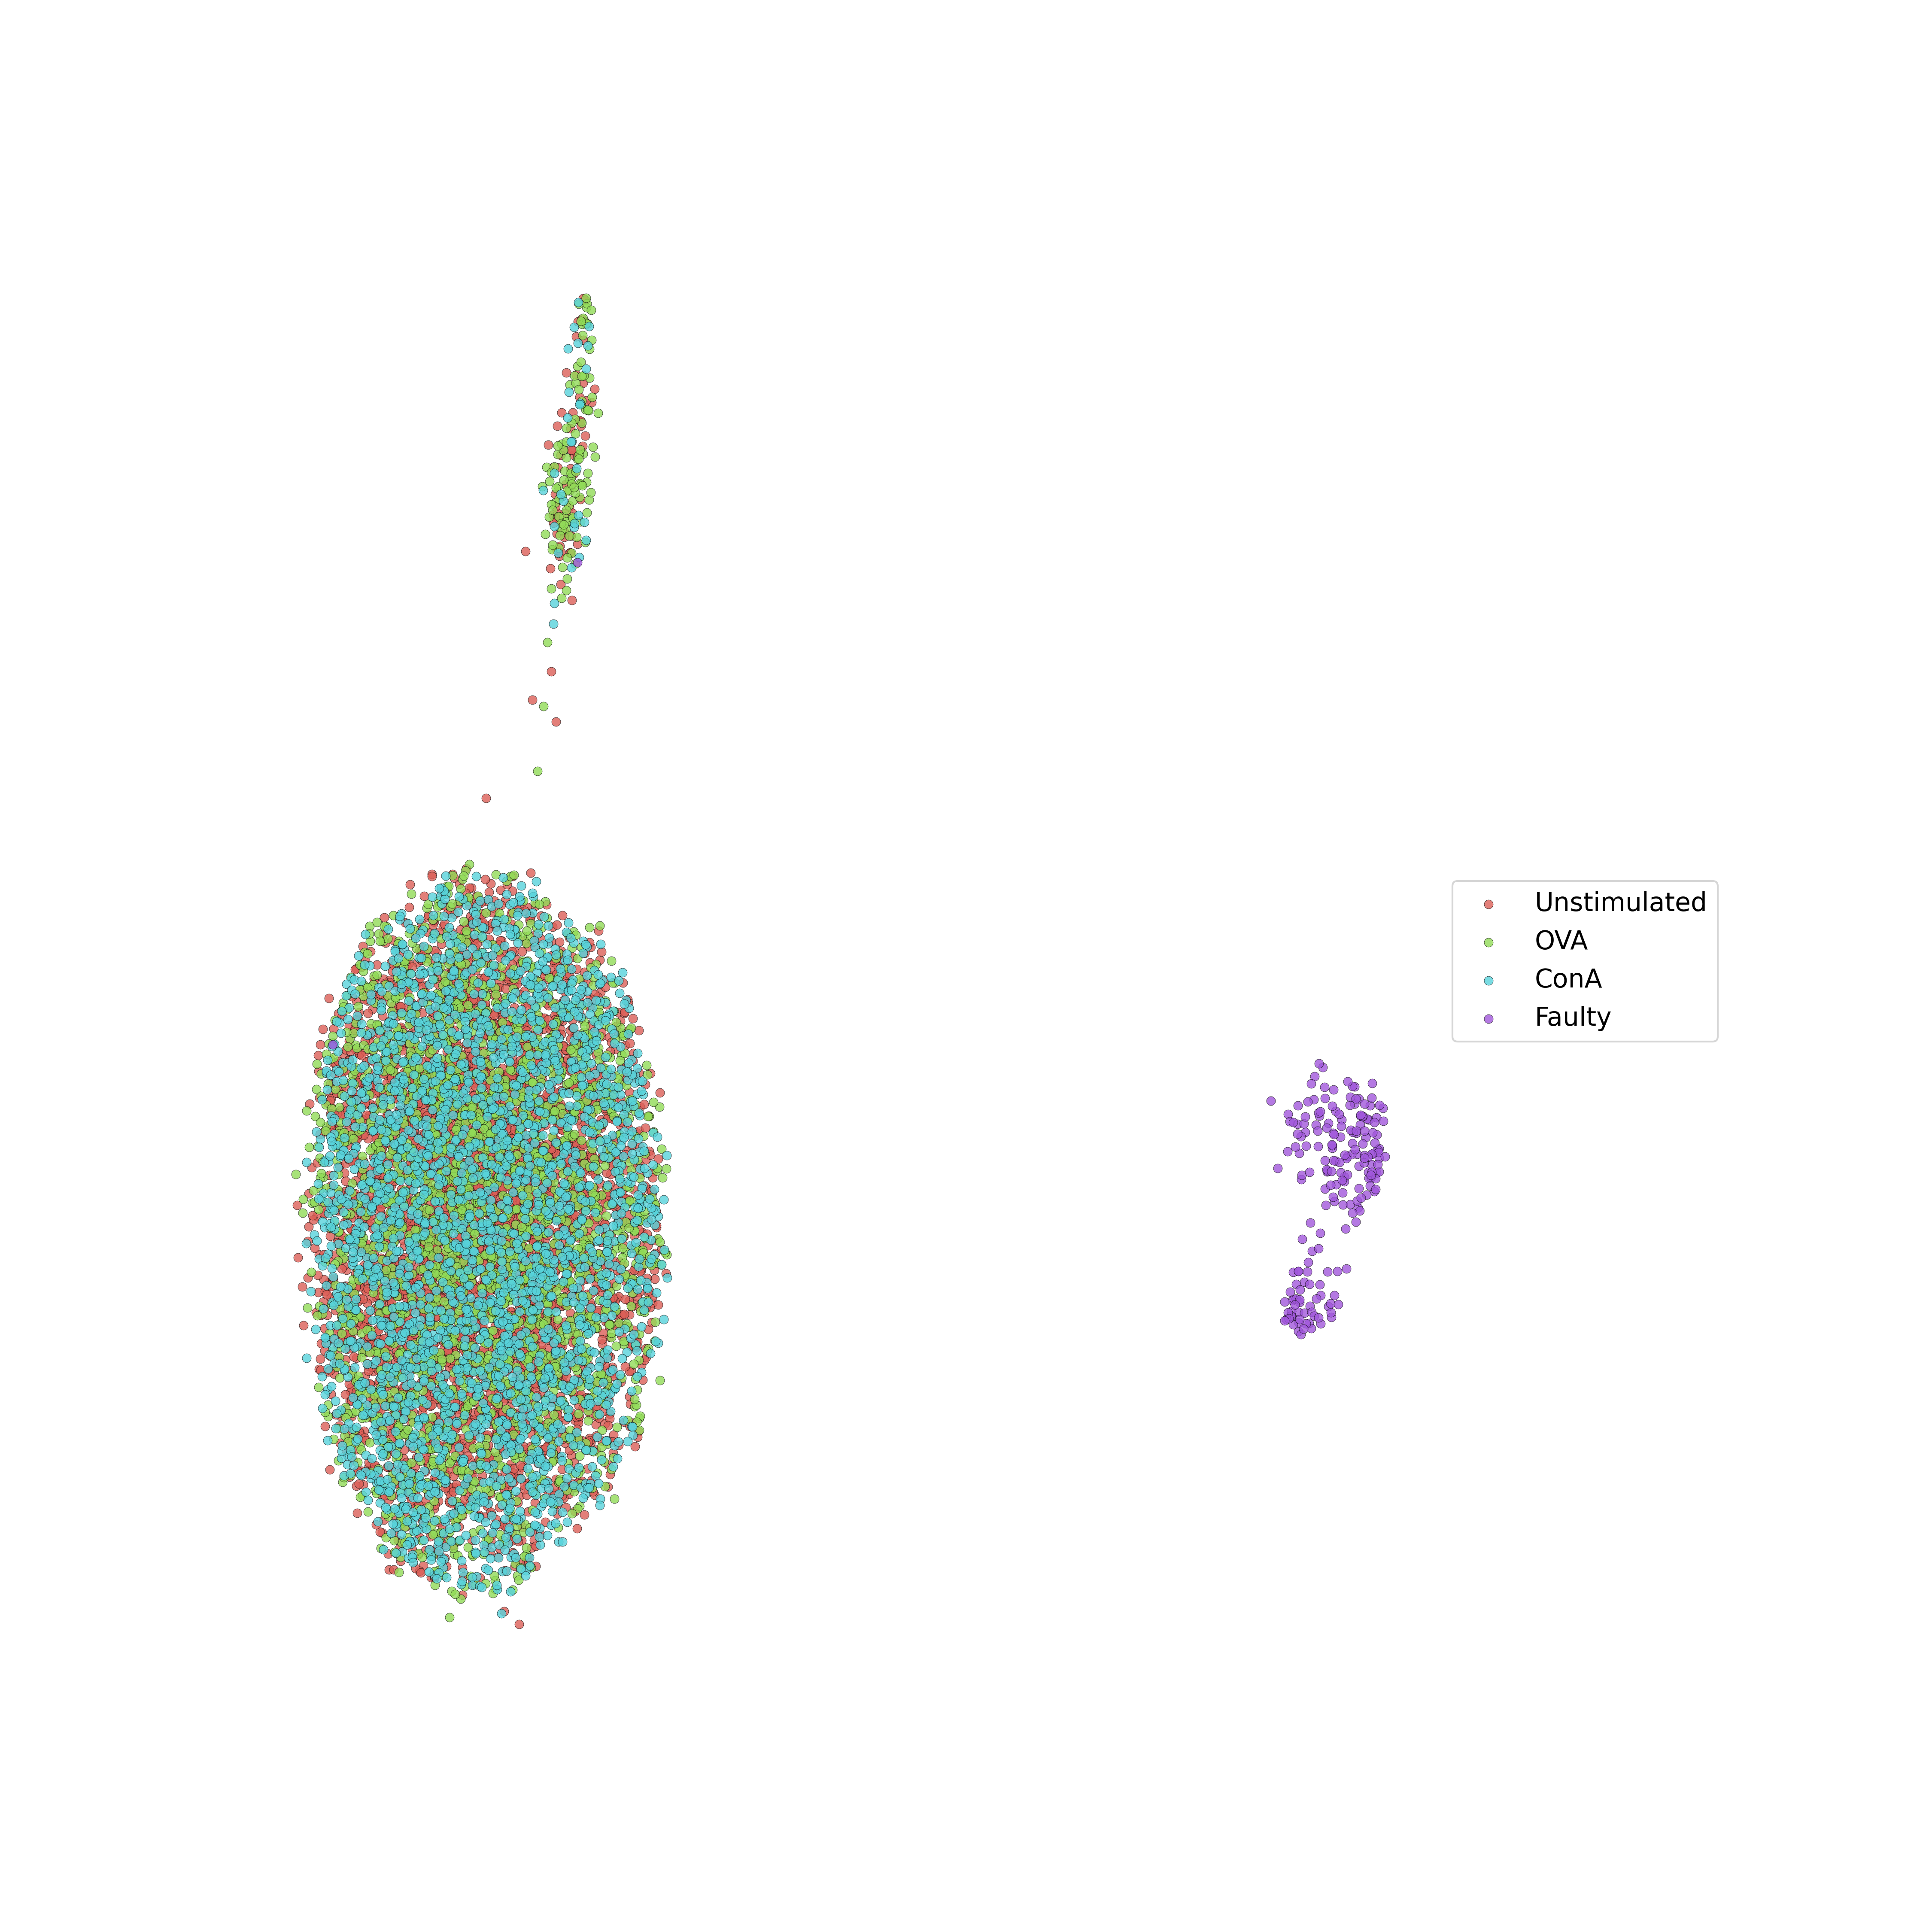
\includegraphics[width=\textwidth]{dissertation/figures/evaluation/DMSO_masked_umap.png}
        \caption{Masked images}
    \end{subfigure}
    \caption{Two-dimensional UMAP projections of the 8,000 test images from the \textbf{DMSO} dataset, which have been noise-corrected (left) and background-corrected (right). UMAP was ran with parameters $n\_neighbors=30$ and $min\_dist=0.8$. The legend highlights which colour corresponds to which stimulation category. In the normal images, the main cluster of points does not show a clear delimitation between images of the same category, however there does seem to be some distinction as we can see a gradient.}
    \label{fig:dmso_projection}
\end{figure}

Every projection highlights that UMAP does not struggle to distinguish \textit{Faulty} images from images containing immune cells. This is useful as it acts as a control that tells us that UMAP is noticing differences in images, and that the autoencoder does not corrupt the images and remove important features. Nonetheless, UMAP did not yield clusters showing any kind of distinction between categories in the cases of the \textbf{full} and \textbf{dual} datasets. A difference is more noticeable in the \textbf{DMSO} dataset. This difference is no longer visible in the masked projection. %This allows us to hypothesise that the experimental conditions used for generating the full and dual datasets do not yield immune cells under different stimulation levels are not structurally different enough in the format they are currently inputted in the dataset, i.e. in small patches of images of size $192\times192\times3$.

\subsection{Are images within the same cluster structurally the same?}

Some projections shown above still showed some clusters and outlier points. We wanted to assess whether the images in these points were indeed structurally similar. In order to explore this, we developed a tool that makes use of matplotlib's animation API\footnote{https://matplotlib.org/api/animation\_api.html}. We can hover over the points of the visualisation to display the original image that is represented by one of the projection points. The drawback of the tool is that it struggles over large clusters of points as it requires quite a lot of memory to update the coordinates in the graph, resize a $192\times192\times3$ image, and display it, and is slow in such cases. 

\begin{figure}[h]
    \centering
    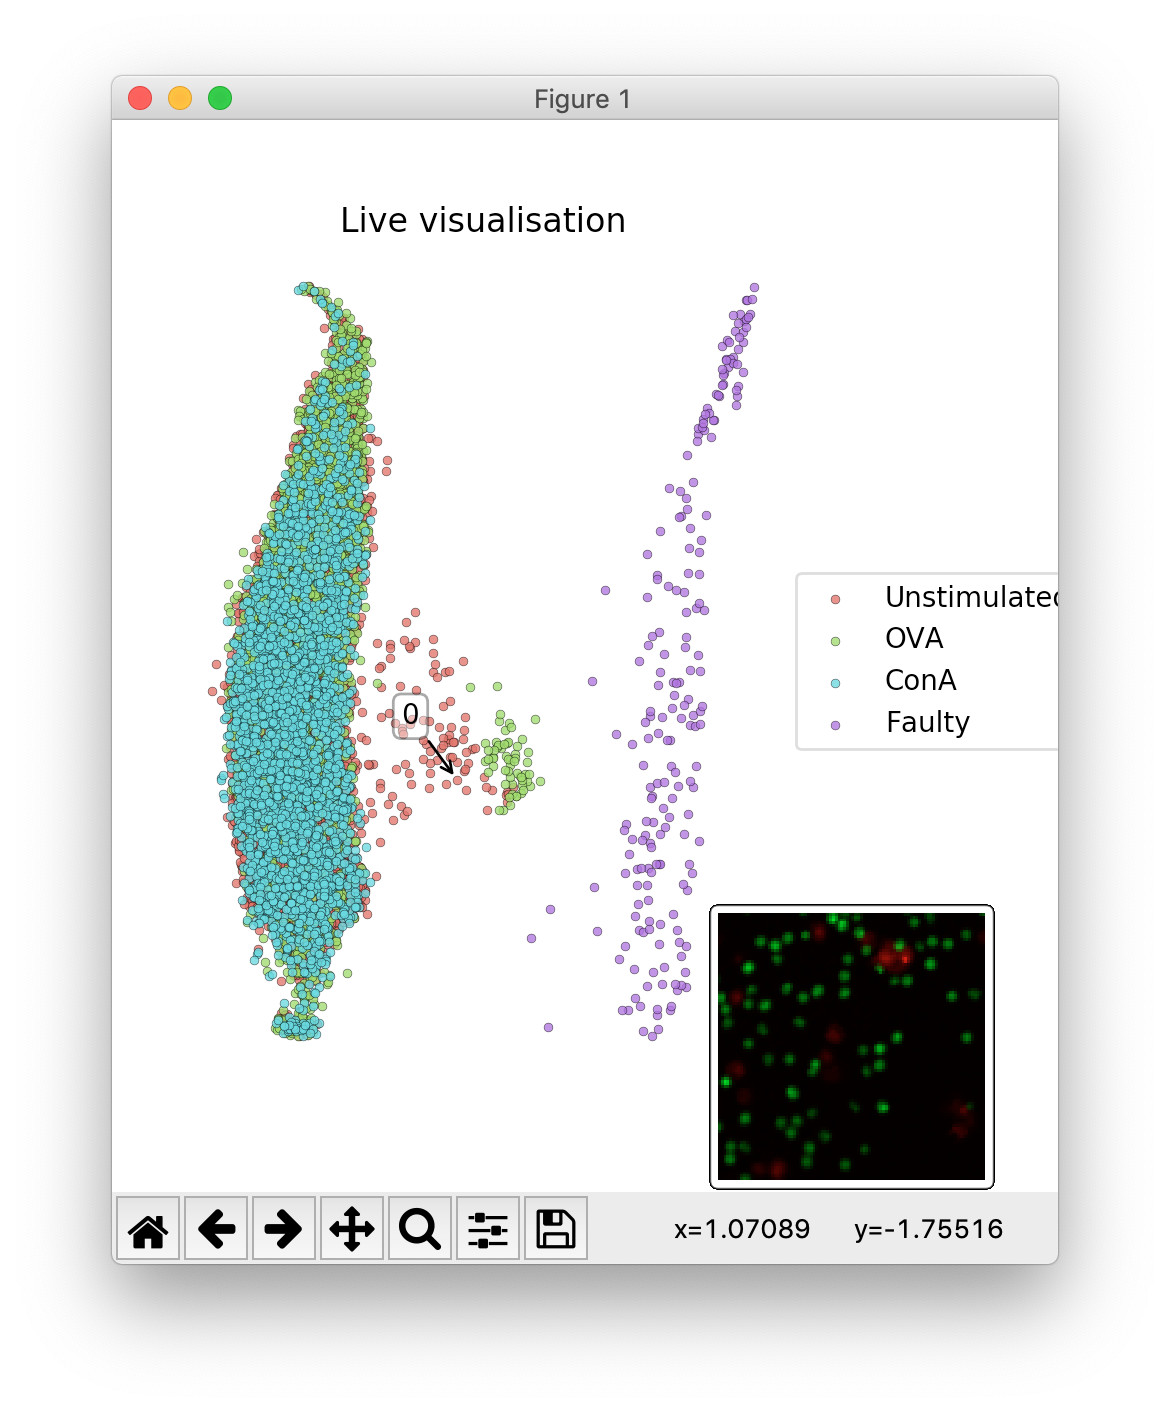
\includegraphics[width=0.32\textwidth]{dissertation/figures/evaluation/right_cluster_big.png}
    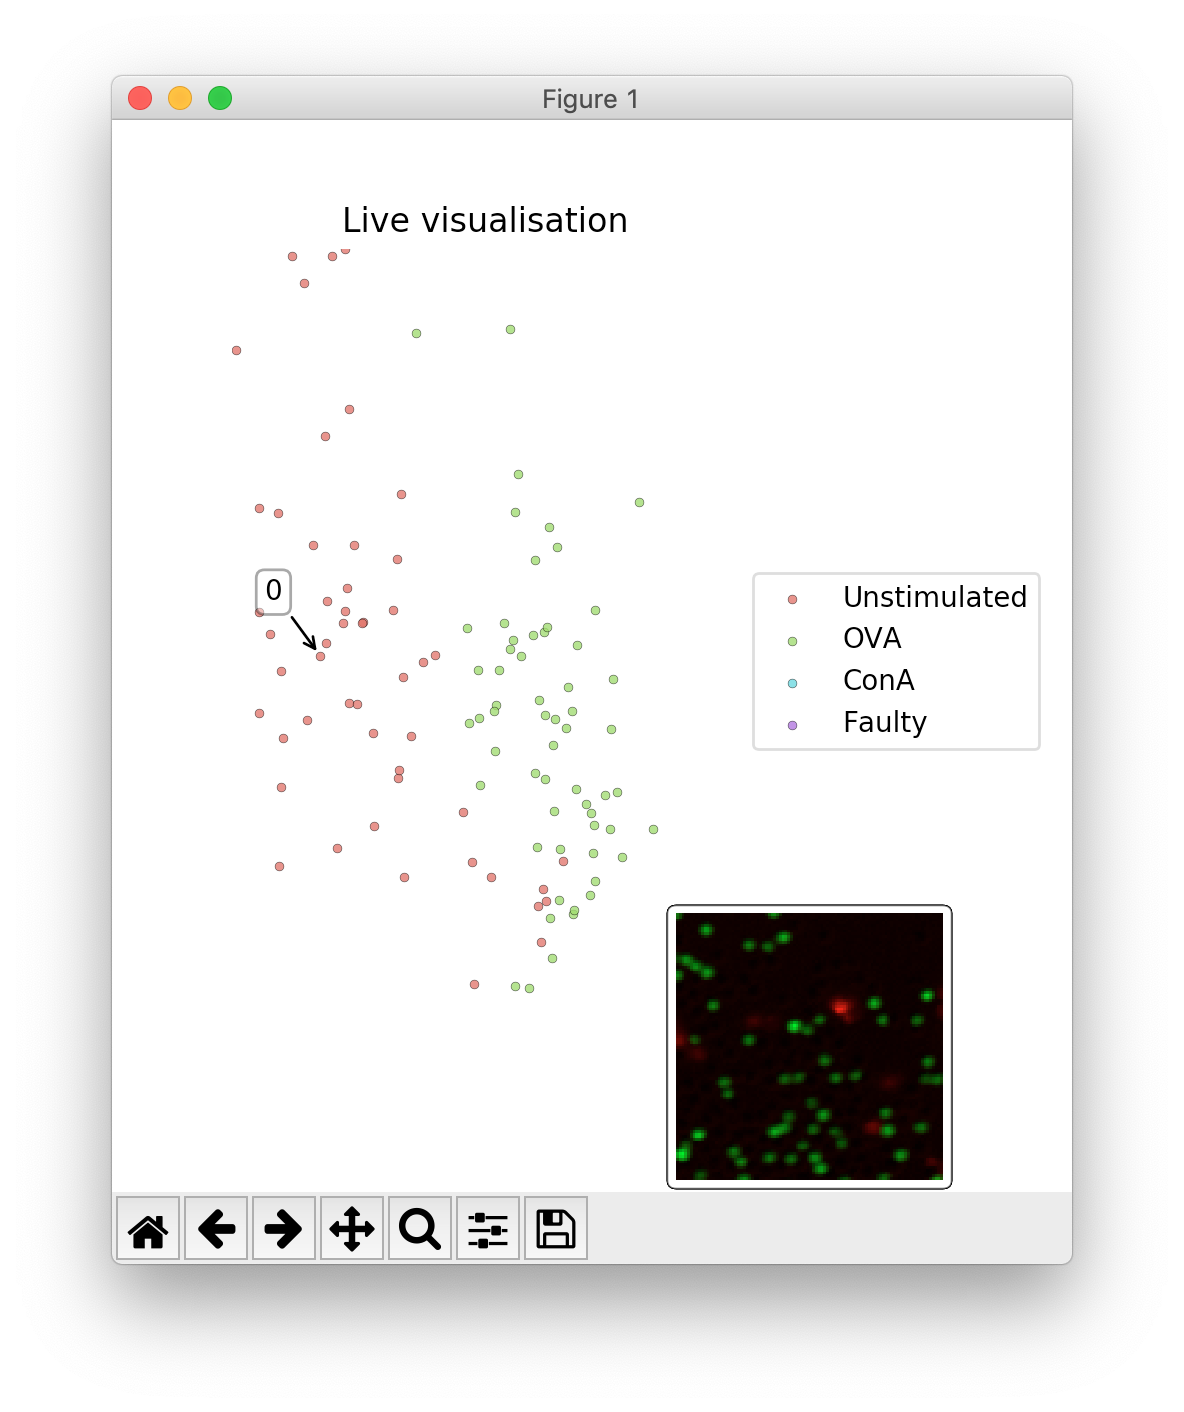
\includegraphics[width=0.32\textwidth]{dissertation/figures/evaluation/right_cluster_red_1.png}
    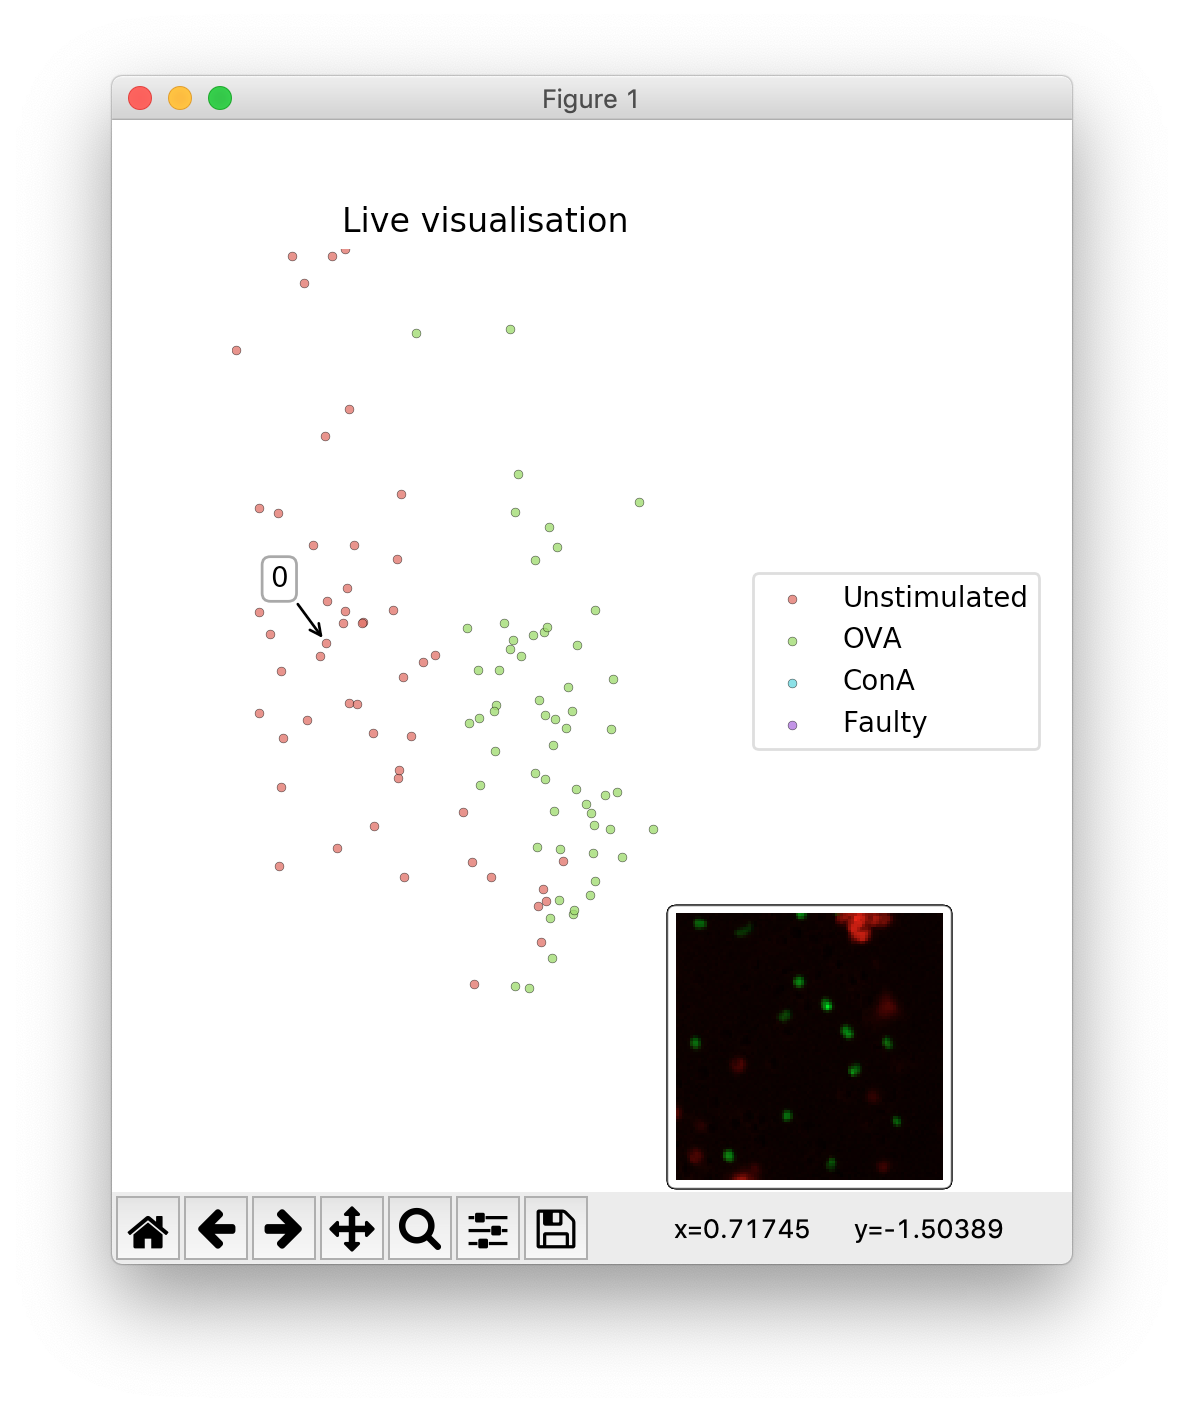
\includegraphics[width=0.32\textwidth]{dissertation/figures/evaluation/right_cluster_red_2.png}
    \caption{Three images extracted from a live visualisation graph of the UMAP projection shown in Figure \ref{fig:dmso_projection}. The graph on the left is unzoomed. The other two graphs have been zoomed in, showing the tool's functionality as well as a closer view of the cluster. We give two example images in the same cluster of similar structure, but one that does not follow the trend.}
    \label{fig:vis_outliers}
\end{figure}

\autoref{fig:vis_outliers} highlight the tool's functionality. We picked the projection of the DMSO dataset from \autoref{fig:dmso_projection} above that showed distinct clusters of images within the same category to evaluate whether or not they were meaningful. The projection in the first image will look slightly different as the plot is of smaller size and the method for drawing the scatter plots had to be adapted for the task. We then zoom over clusters of interest to be able to pick out points more efficiently. This view shows us that we can find two images within the same cluster that look structurally the same, but another image which does not is also in that same structure. 

\autoref{fig:vis_outliers_2} shows a different case. We highlight three points in a cluster which are close to each other and show they are similar – they all are a particular hue of green. This highlights that our noise correction was not necessarily successful in all cases, and explains why less clusters are found with the masked images. 

\begin{figure}[h]
    \centering
    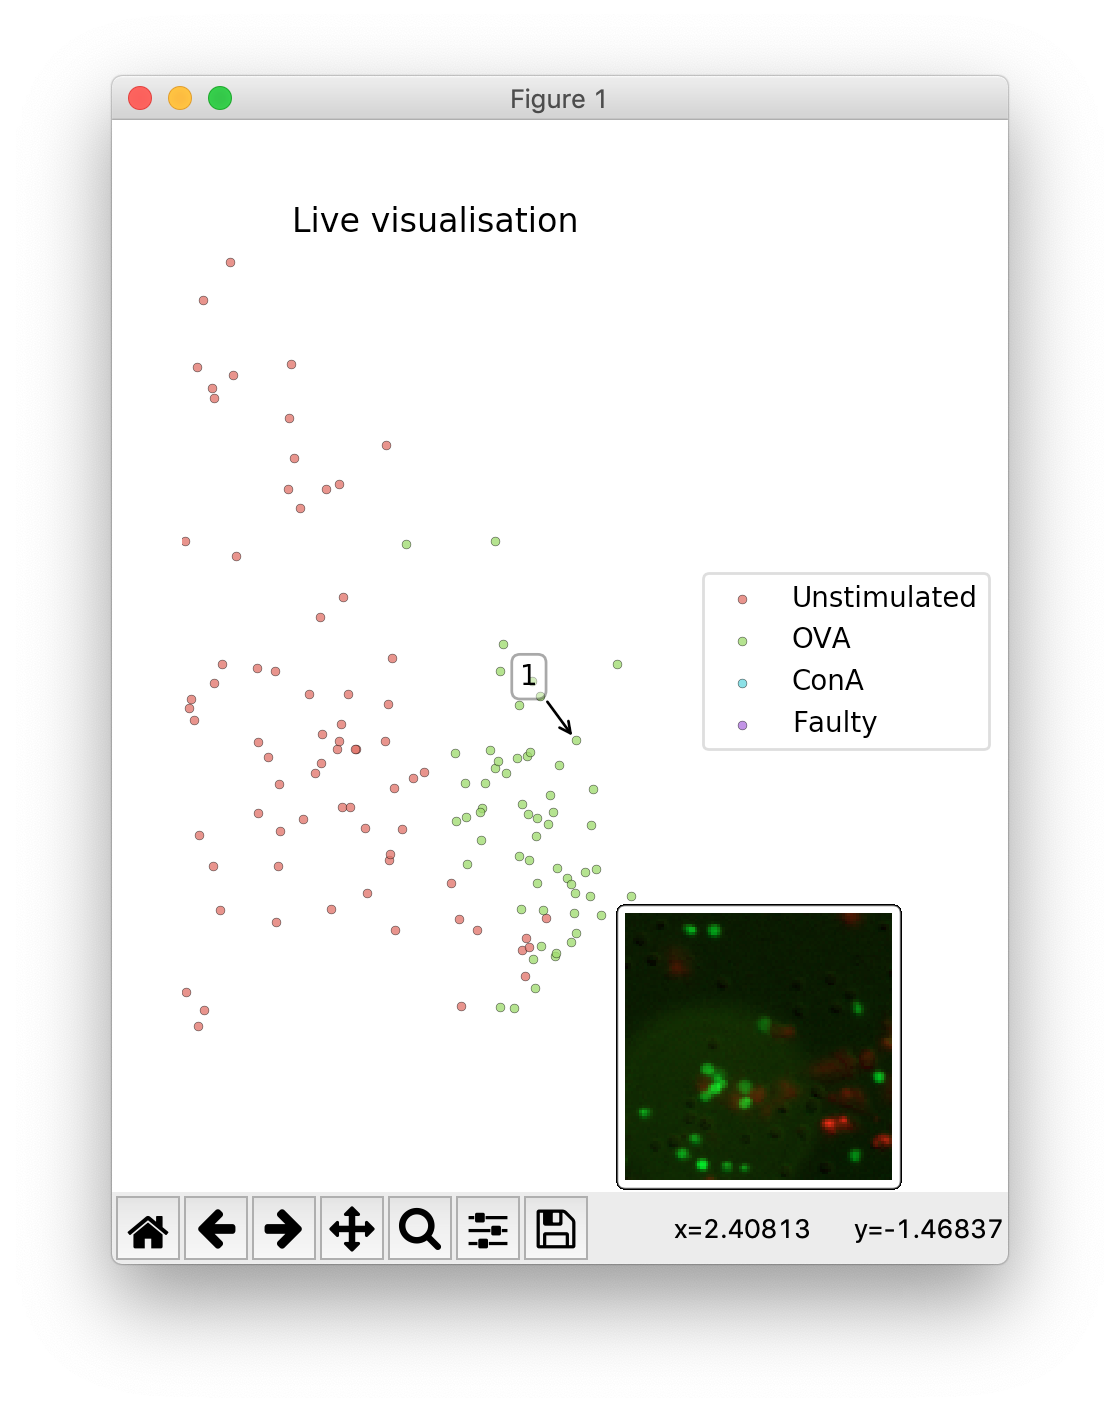
\includegraphics[width=0.32\textwidth]{dissertation/figures/evaluation/green_cluster_1.png}
    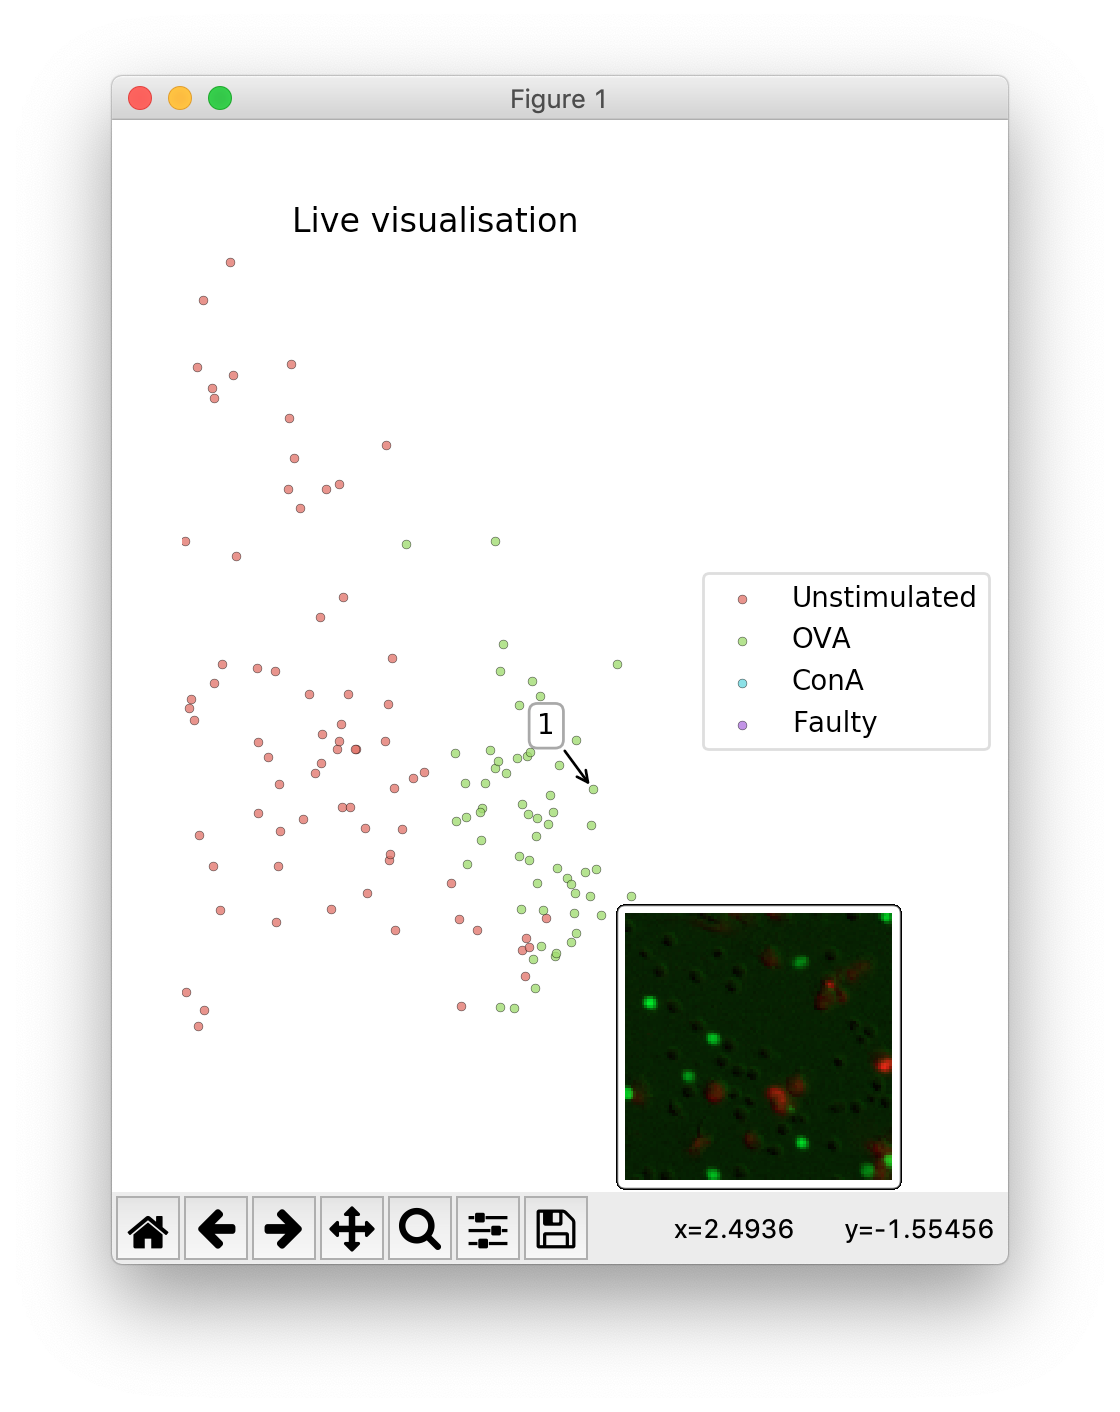
\includegraphics[width=0.32\textwidth]{dissertation/figures/evaluation/green_cluster_2.png}
    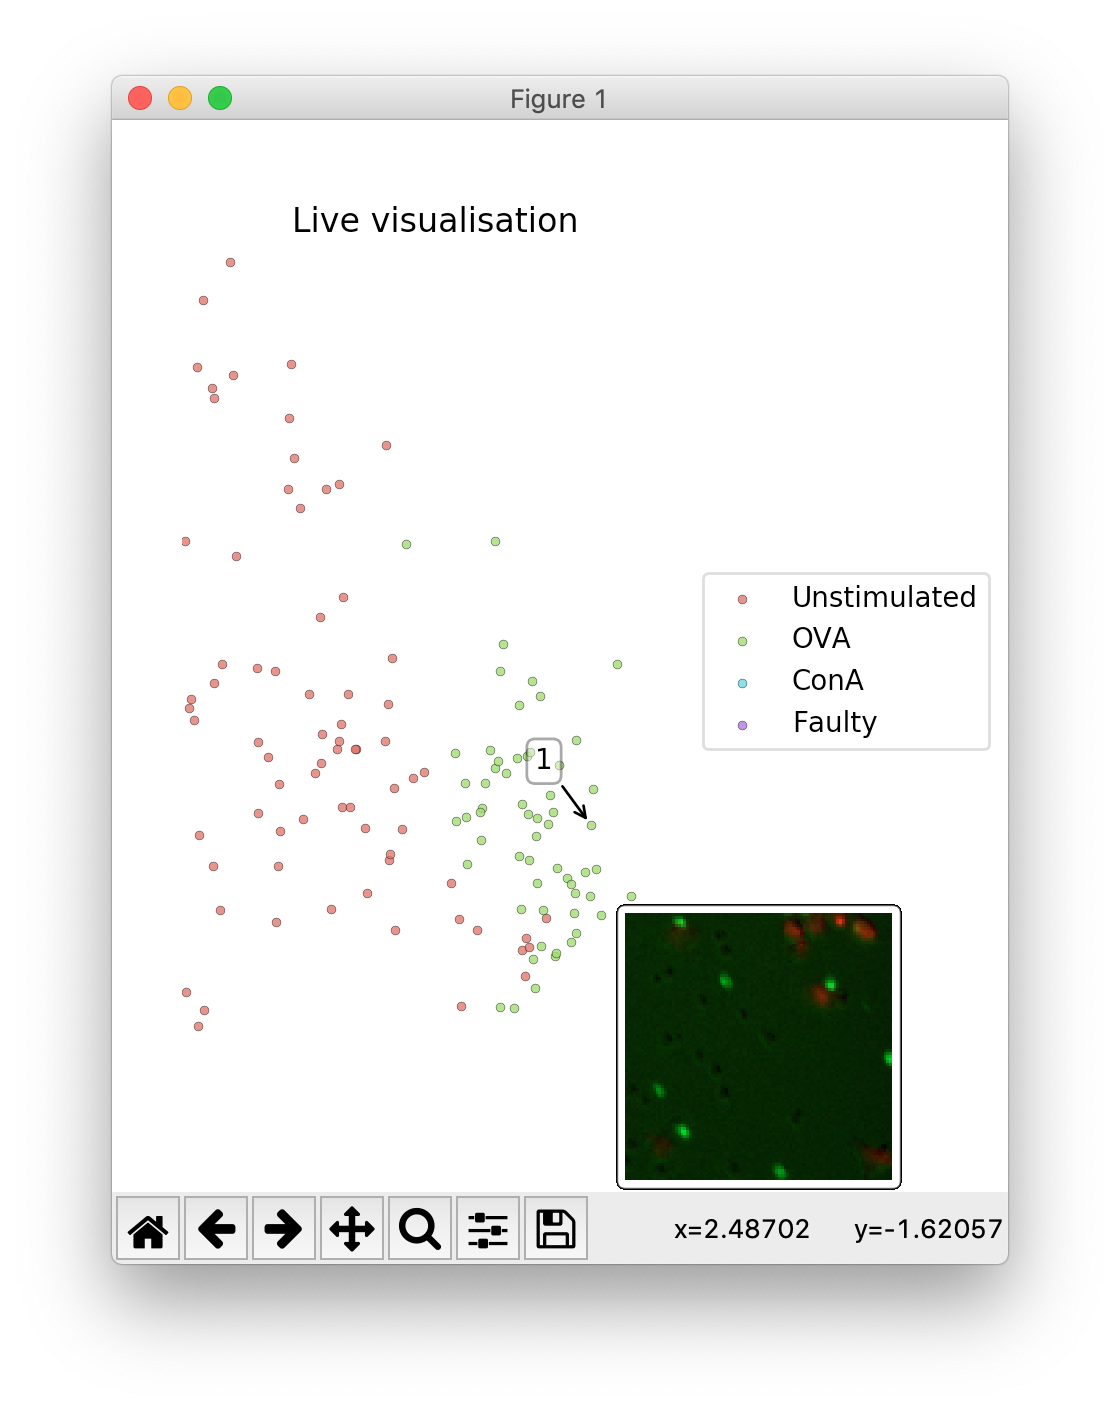
\includegraphics[width=0.32\textwidth]{dissertation/figures/evaluation/green_cluster_3.png}
    \caption{Three images extracted from a live visualisation graph of the UMAP projection shown in \autoref{fig:dmso_projection}. The graph has been zoomed in to the distinctive green cluster. This highlights three images that are similar – they are all a shade of green.}
    \label{fig:vis_outliers_2}
\end{figure}

\subsection{Are our visualisations more meaningful with interaction measure meta-data?}

In the case of visualisations that did yield some groupings, but contained points of mixed categories, we hypothesised that other meta-data about the images might explain why some clusters were formed. Indeed, maybe the stimulation level of immune cells was not creating enough distinction between images, and they were more influenced by something else. For example, how much the cells overlapped in the image, regardless of their stimulation category. 

We plotted the visualisations again, but using the interaction measures collected with the intersection-over-union metric to change the size of the markers. We decided to tweak the visualisations shown in Figure \ref{subfig:full_projection_normal} and Figure \ref{subfig:dual_projection_masked} as they yielded some separated groupings, but of mixed labels. The results are shown in \autoref{fig:size_visualisation} below. 

\begin{figure}[h!]
    \centering
    \begin{subfigure}{.45\textwidth}
        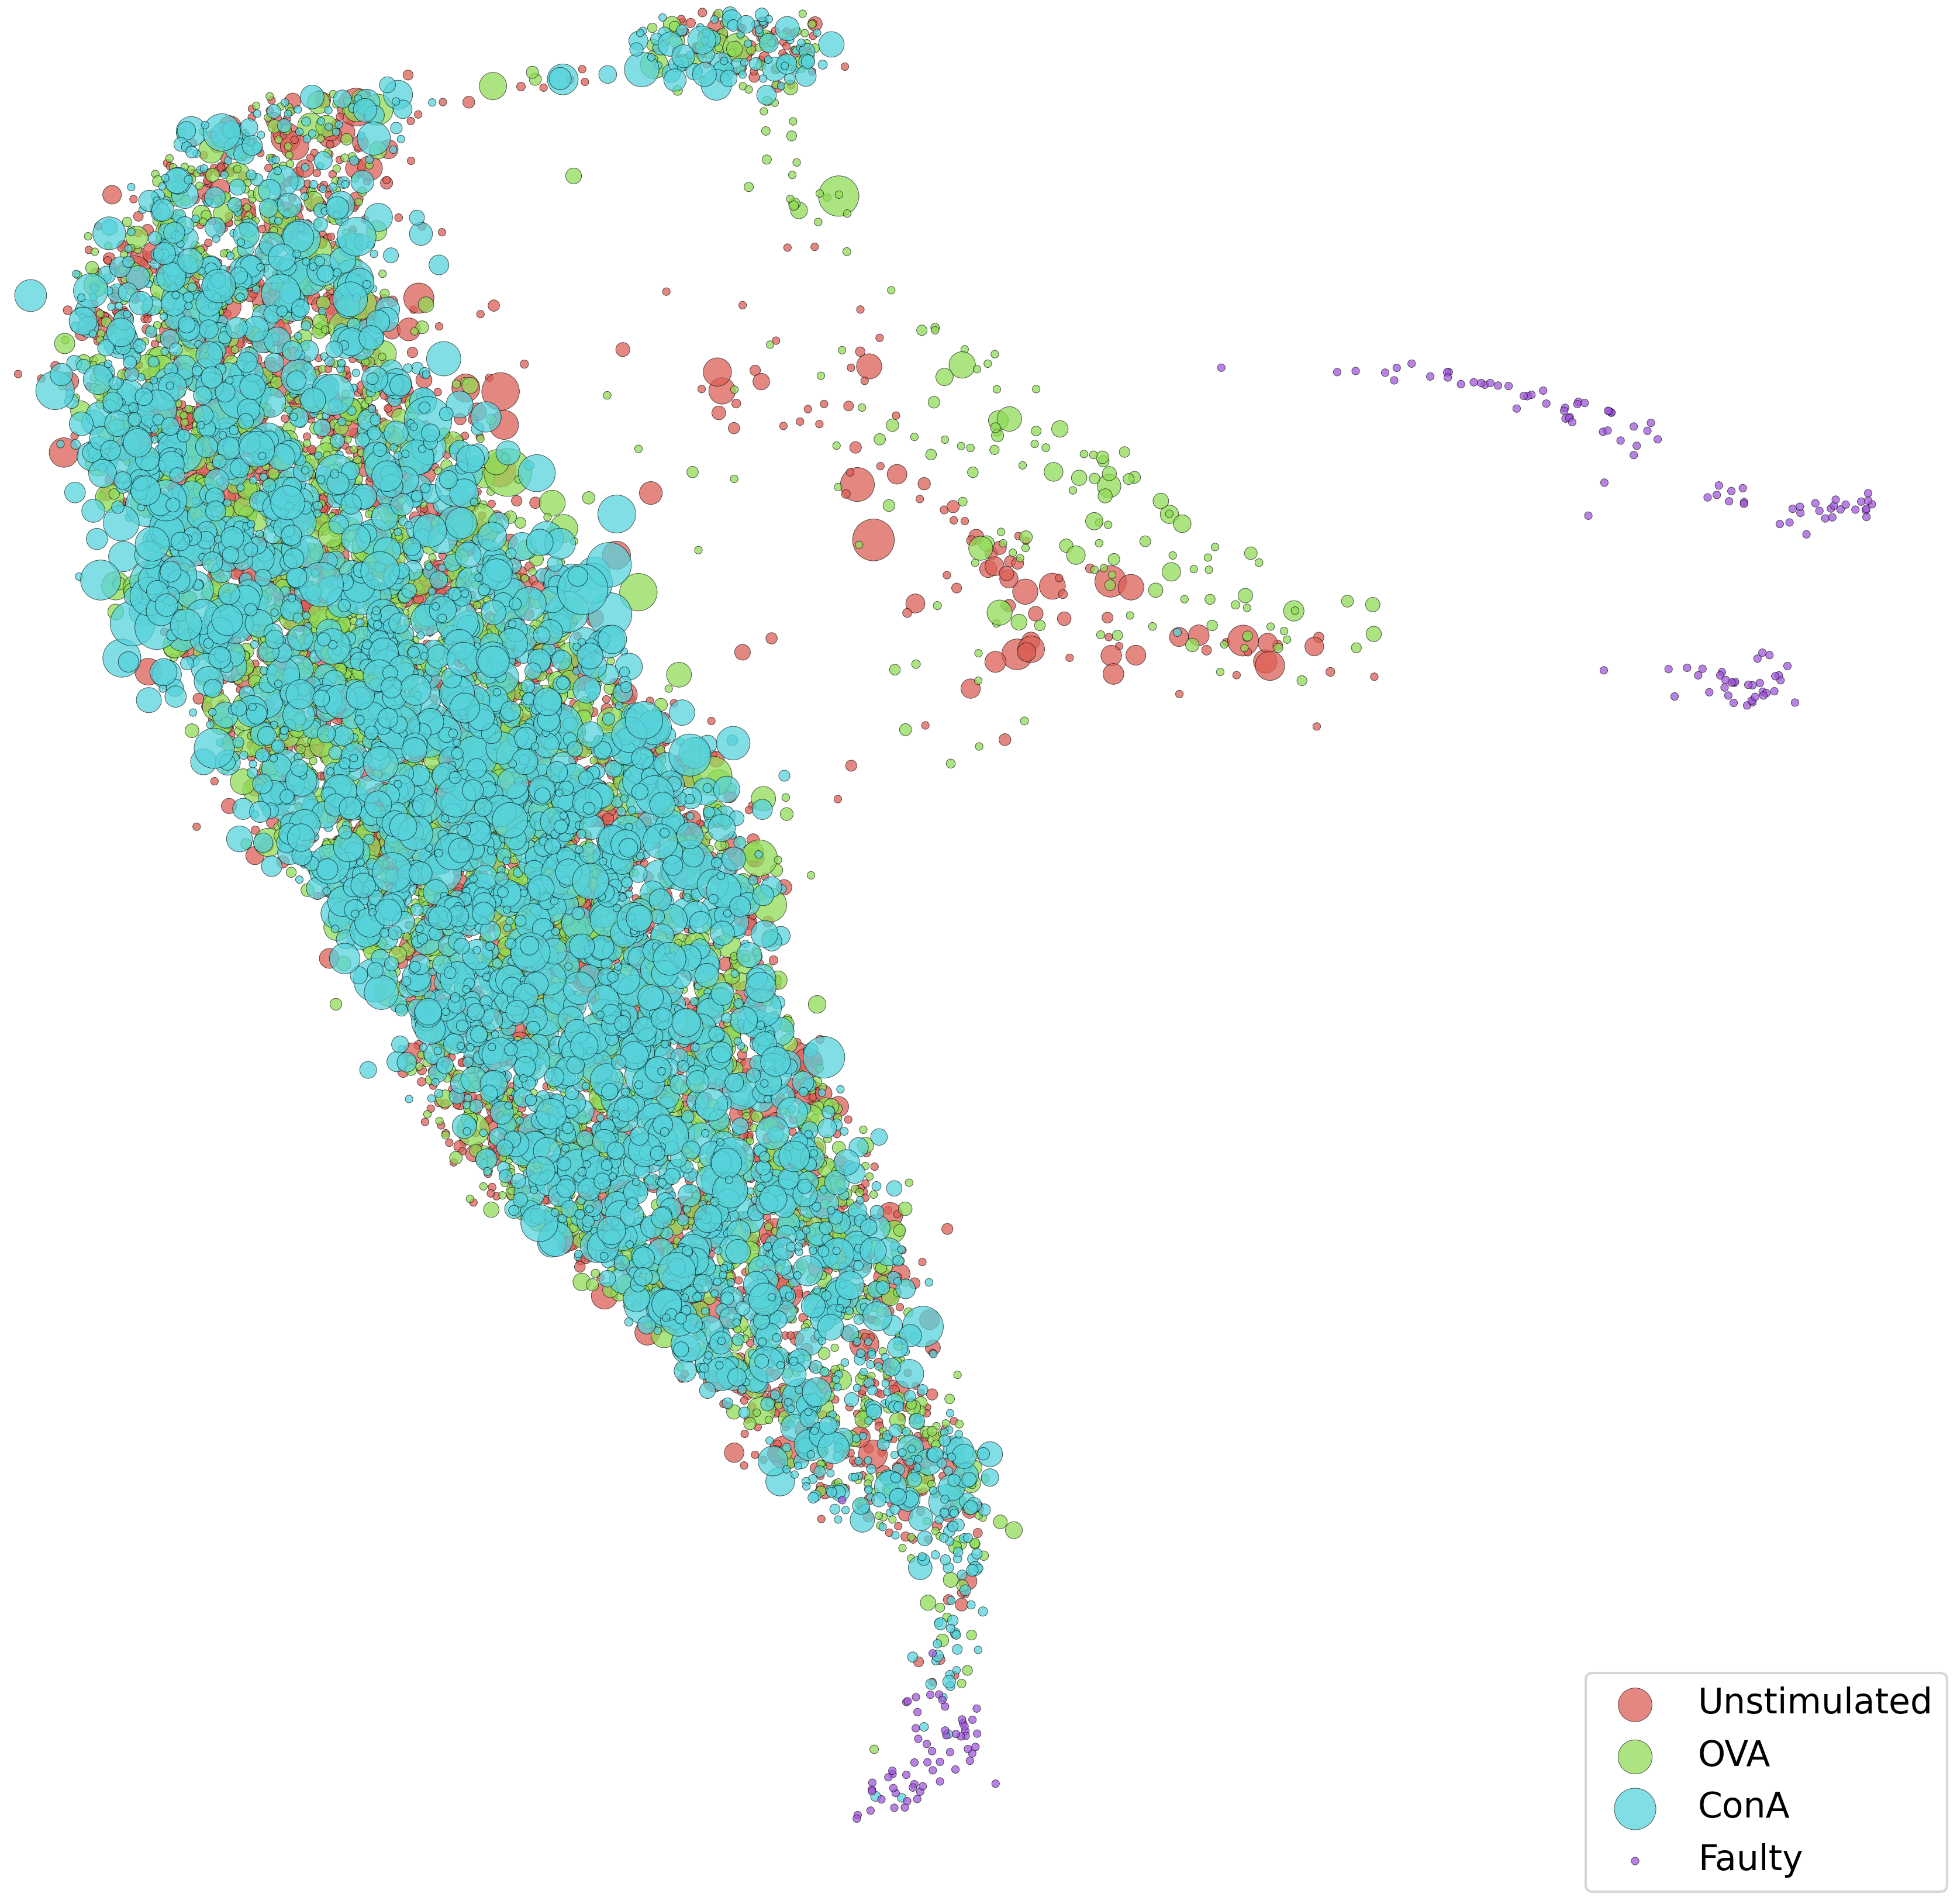
\includegraphics[width=\textwidth]{dissertation/figures/evaluation/CK19_umap_size.png}
        \caption{UMAP projection of the full dataset}
    \end{subfigure}
    \begin{subfigure}{.45\textwidth}
        \includegraphics[width=\textwidth]{dissertation/figures/evaluation/CK22_masked_umap_size.png}
        \caption{UMAP projection of the masked dual dataset}
    \end{subfigure}
    \caption{UMAP projections for the full dataset and masked dual dataset, tweaked with the size of overlap in each image as the size of the scatter points. The legend shows the category of each point as well as the average size of the points.}
    \label{fig:size_visualisation}
\end{figure}

These visualisations show us that although all images in the separated clusters contain a similar level of interaction, some other images in the main clusters also have that level of interaction. As such, we also cannot say that UMAP is finding structure in the images based on how much overlap (i.e. shades of orange) there is.

\section{Regression}

Our regression task is to predict the percentage of overlap between T-cells and dendritic cells from an image where T-cells are shaded green, and dendritic cells are shaded red.

\subsection{Metrics}

Our regression model is trained on mean squared error (MSE). We decided to evaluate on root-mean-square-error (RMSE) as it is a common metric for evaluating the difference between predictions of a model and actual truth values: RMSE has the advantage of being in the same unit as the dependent variable. In our case the unit is the percentage of overlap between the cells objects obtained with intersection-over-union. RMSE is defined as the square root of the quadratic mean of the difference between our predicted values and their truth values. The equation is as follows:

\begin{equation}
    RMSE = \sqrt{\frac{1}{n}{\Sigma_{i=1}^{n}{\Big({\hat{y}_i-y_i})}^2}}
\end{equation}

where $n$ is the number of samples in the dataset, $y$ is the true value of a sample, and $\hat{y}$ is the predicted value of a sample. 

We also include the (unbiased) standard deviation (SD) of our predicted results to express their variability. The formula for SD is as follows:

\begin{equation}
    \sigma = \sqrt{\frac{1}{n-1}\Sigma_{i=1}^{n}{(\hat{y}_i - \mu)}^2}
\end{equation}

where $n$ is the number of predicted samples, $\hat{y}_i$ is the predicted value of a sample and $\mu$ is the mean of all predicted values. 

\subsection{Can we quantify interaction from an image of immune cells?}

We evaluate the predictions made by the normal and masked regression models by looking at the predictions of each dataset in each stimulation category, however the model was not fed any stimulation category labels during training. Nonetheless, we might see more overlap across different stimulation categories if they generate more interaction between immune cells, so it is important to also look at errors in prediction within those ranges of values.

\bigskip
\subsubsection{Full dataset}
\hfill
\hfill 

Our regression model reports an overall score of 1.838 $\pm$ 4.583 on the test instances of the full dataset. The masked regression model trained on the images which have a black background reports a score of 1.161 $\pm$ 4.732, which shows an improvement in RMSE. Variance in the true values is of 4.853 overall, meaning that we can see a very similar amount of variance in the predicted values. Table \ref{tab:full_rmse} reports the full scores on all stimulation categories. 

\begin{table}[h!]
\centering
\caption{Average RMSE and SD scores (in \%) for the regression model's predictions on the \textbf{full} dataset. The closer the value is to 0, the closer the prediction is. We can see that the difference remains quite low across all datasets, with ConA having the highest RMSE and SD.}
\label{tab:full_rmse}
\begin{tabular}{l|rrr|r}
\rowcolor[HTML]{EFEFEF}
\textbf{Images} & \cellcolor[HTML]{FFCCC9}\textbf{Unstimulated} & \cellcolor[HTML]{C9FFCB}\textbf{OVA} & \cellcolor[HTML]{96FFFB}\textbf{ConA} & \textbf{All} \\ \hline
Normal      & 1.344 $\pm$ 3.102  & 1.387 $\pm$ 2.963   & 2.502 $\pm$ 6.004  &   1.838 $\pm$ 4.583  \\ \hline
Masked      &    0.832 $\pm$ 3.174          & 0.766 $\pm$ 3.355  &  1.642 $\pm$ 6.067   &   1.161 $\pm$ 4.732 
\end{tabular}
\end{table}

We can see that the \textit{ConA} category has a higher RMSE score, while \textit{Unstimulated} and \textit{OVA} scores are similar. Given the large standard deviations on each of the scores, the differences between them for each different stimulation category cannot be considered statistically significant. The high standard deviation for images with \textit{ConA} stimulation could be partly explained with the range of values for that category. 

\begin{figure}[h!]
    \centering
    \begin{subfigure}{.8\textwidth}
        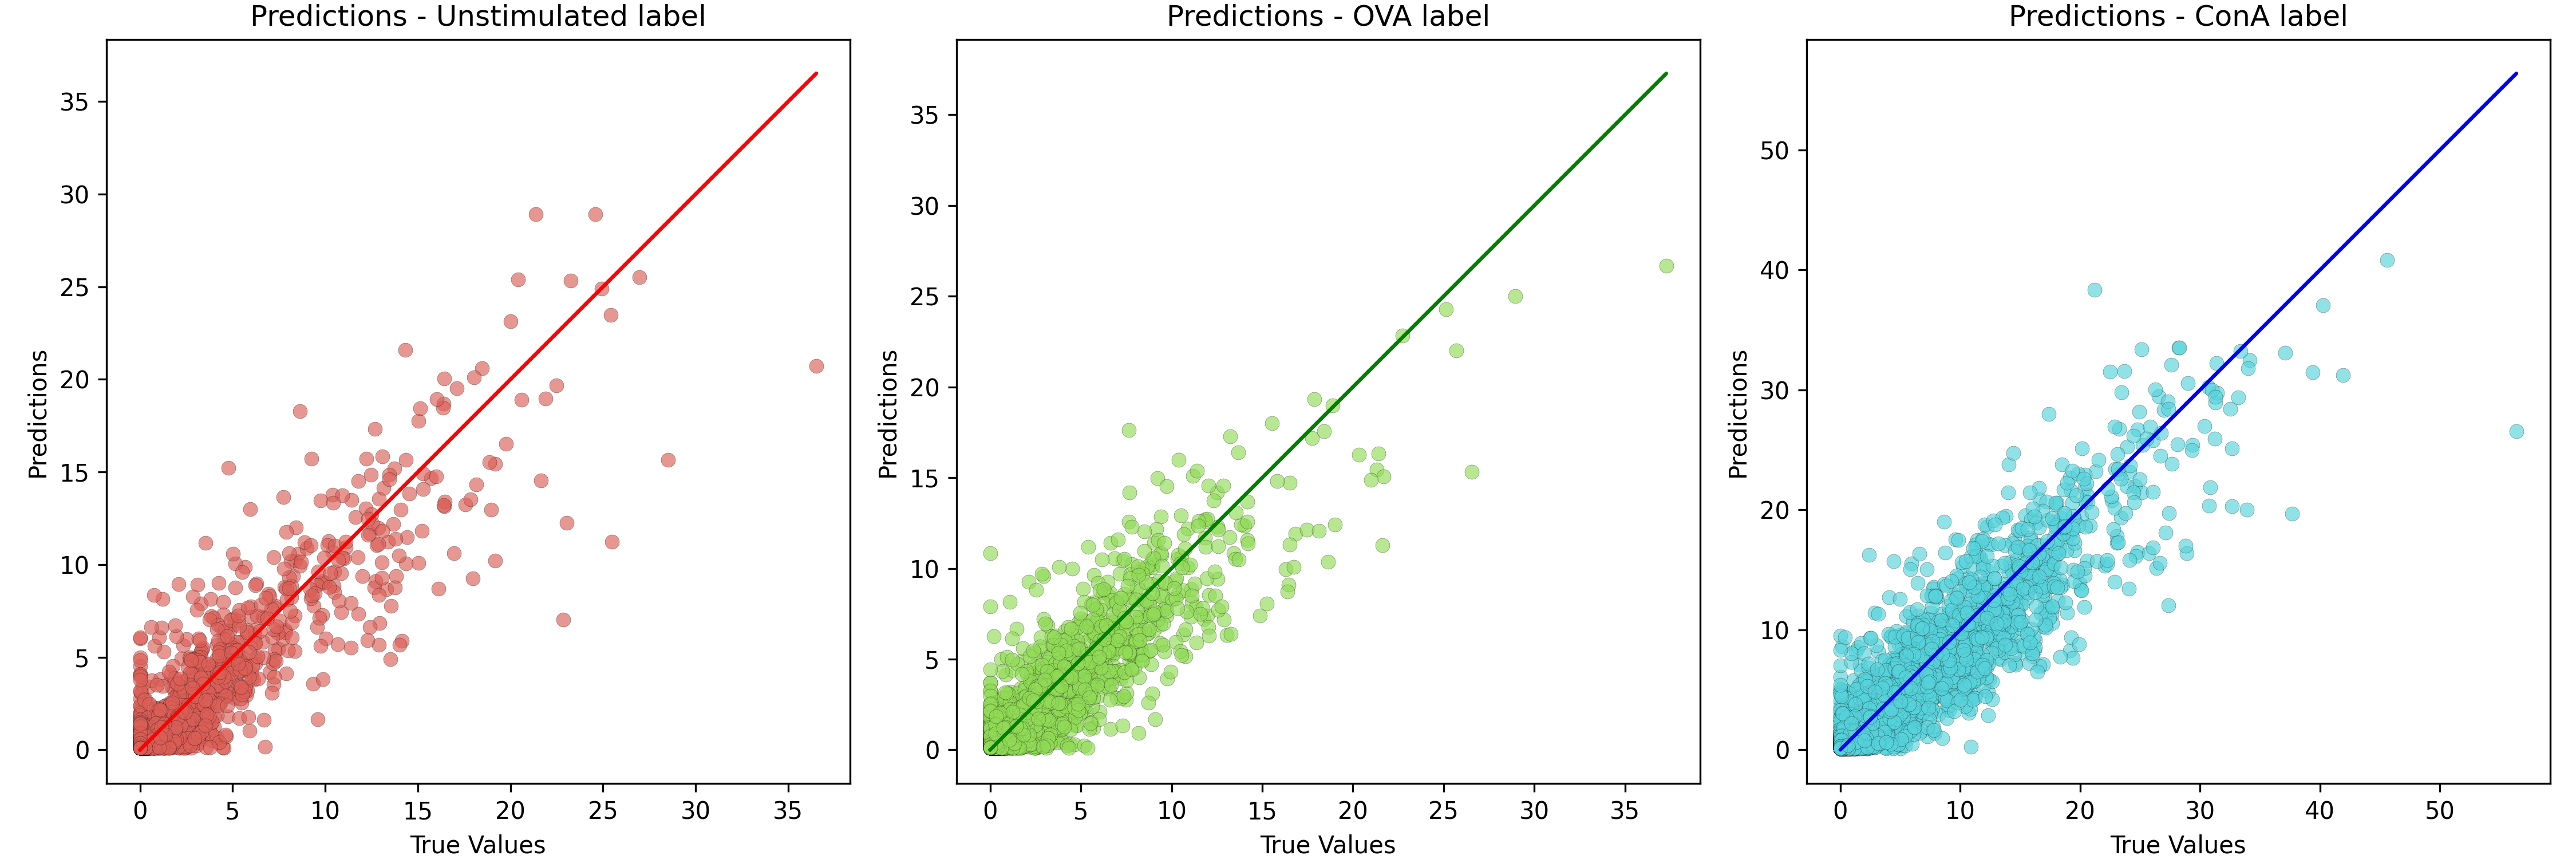
\includegraphics[width=\textwidth]{dissertation/figures/evaluation/CK19_scatter.png}
        \caption{Normal images}
    \end{subfigure}
    \begin{subfigure}{.8\textwidth}
        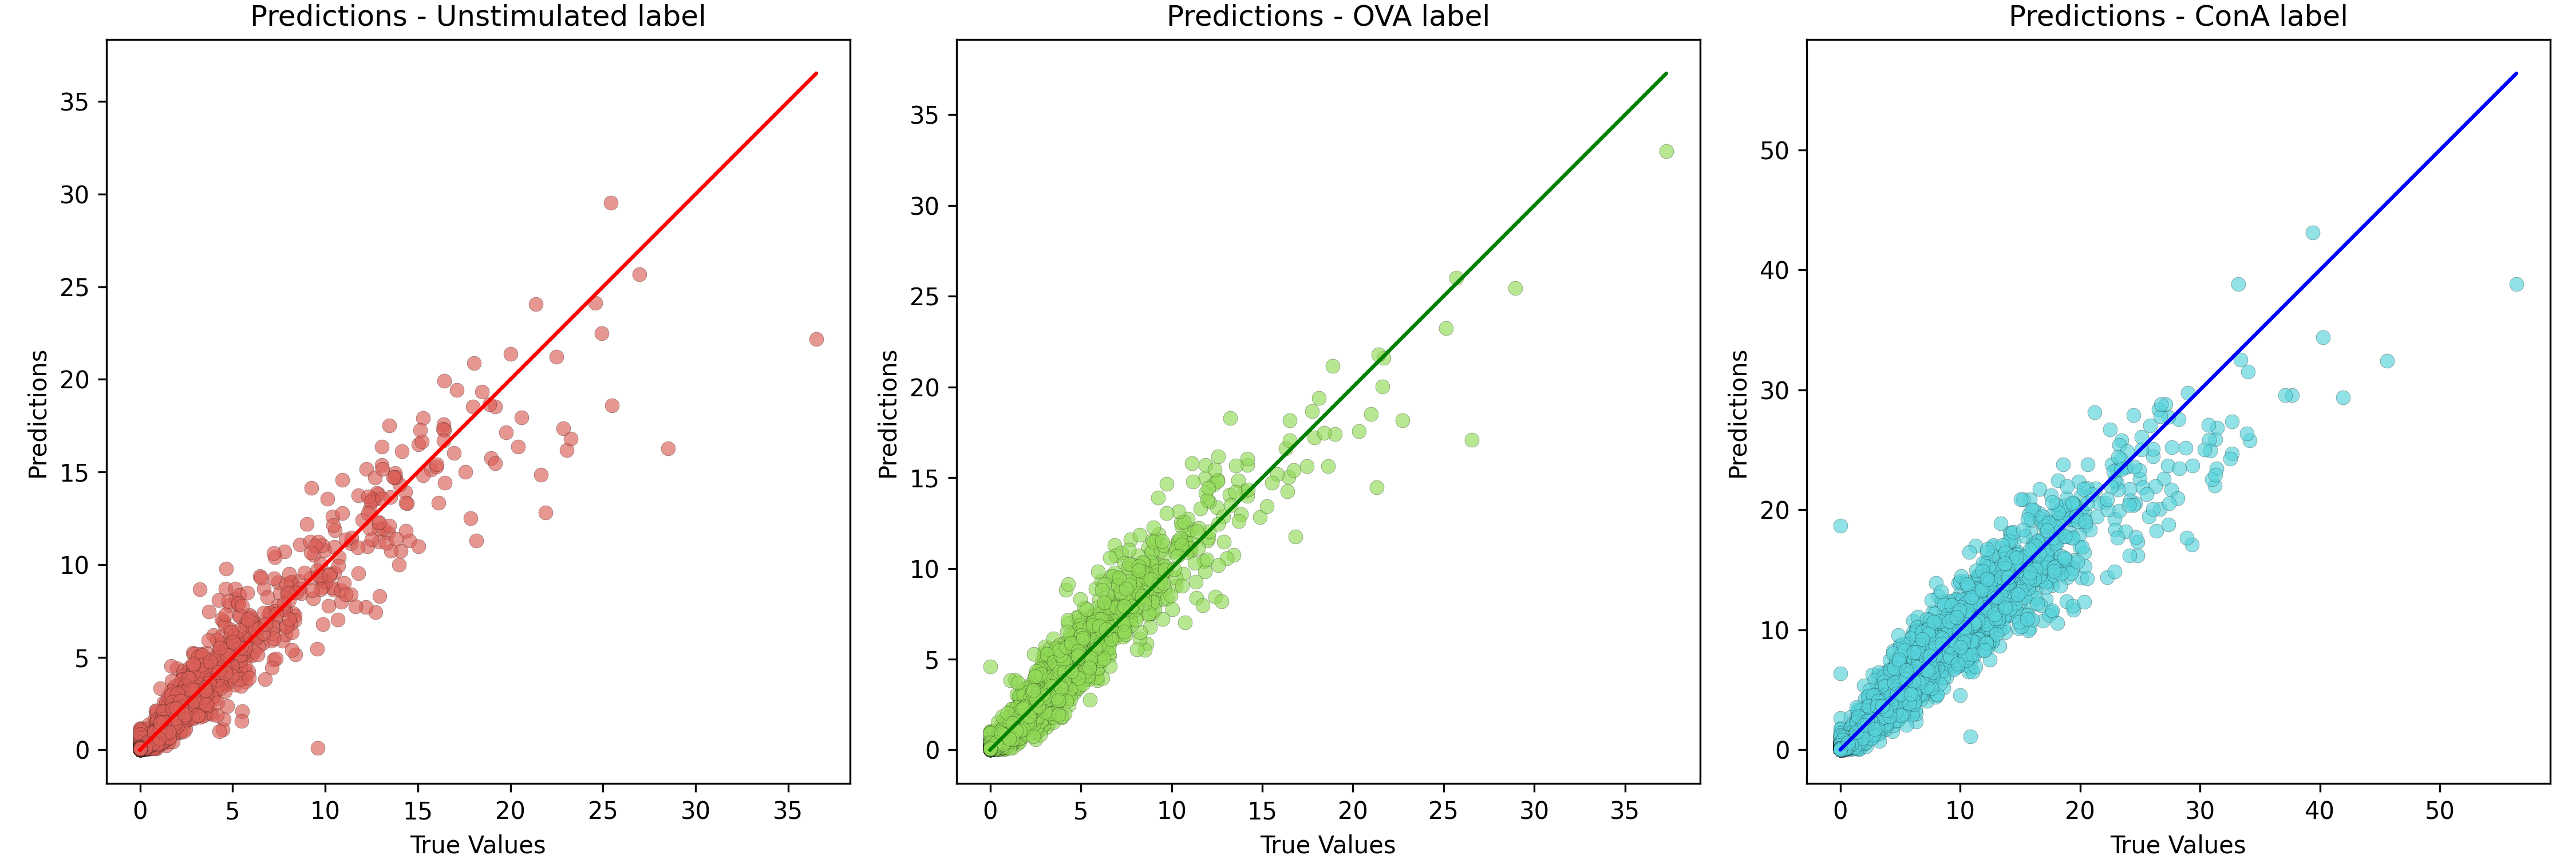
\includegraphics[width=\textwidth]{dissertation/figures/evaluation/CK19_masked_scatter.png}
        \caption{Masked images}
        \label{fig:full_masked_scatter}
    \end{subfigure}
    \caption{Scatter plot comparing true values (x-axis) to predicted values (y-axis) for the \textbf{full} dataset. The line of best fit is the straight continuous line running diagonally true the plot, which is the line we want our predictions on. The predictions are plotted for, from left to right: Unstimulated (red), OVA (green), and ConA (blue). Each sub-plot is not on the same scale as each category does not have the same range of overlap values, but we wanted to show more granularity for each sub-plot.}
    \label{fig:full_scatter}
\end{figure}

Figure \ref{fig:full_scatter} is a scatter plot showing the line of best fit for our predictions. In the ideal scenario, where the regression model always makes the right prediction, each point should be placed on the diagonal line. We can see that that in the \textit{Unstimulated} category, points struggle to follow this line. There is a large number of errors when the value to predict is closer to 0. This is also the case for the \textit{OVA} and \textit{ConA} categories, although less so. Furthermore, the plot shows that images in the \textit{ConA} category have a higher percentage of overlap in general. This could explain why the \textit{ConA} category yields a higher RMSE and SD score. In fact, if more points in the \textit{Unstimulated} and \textit{OVA} categories have an overlap value of 0, then it would explain why they have a smaller RMSE and SD score. 

\begin{figure}[h!]
    \centering
    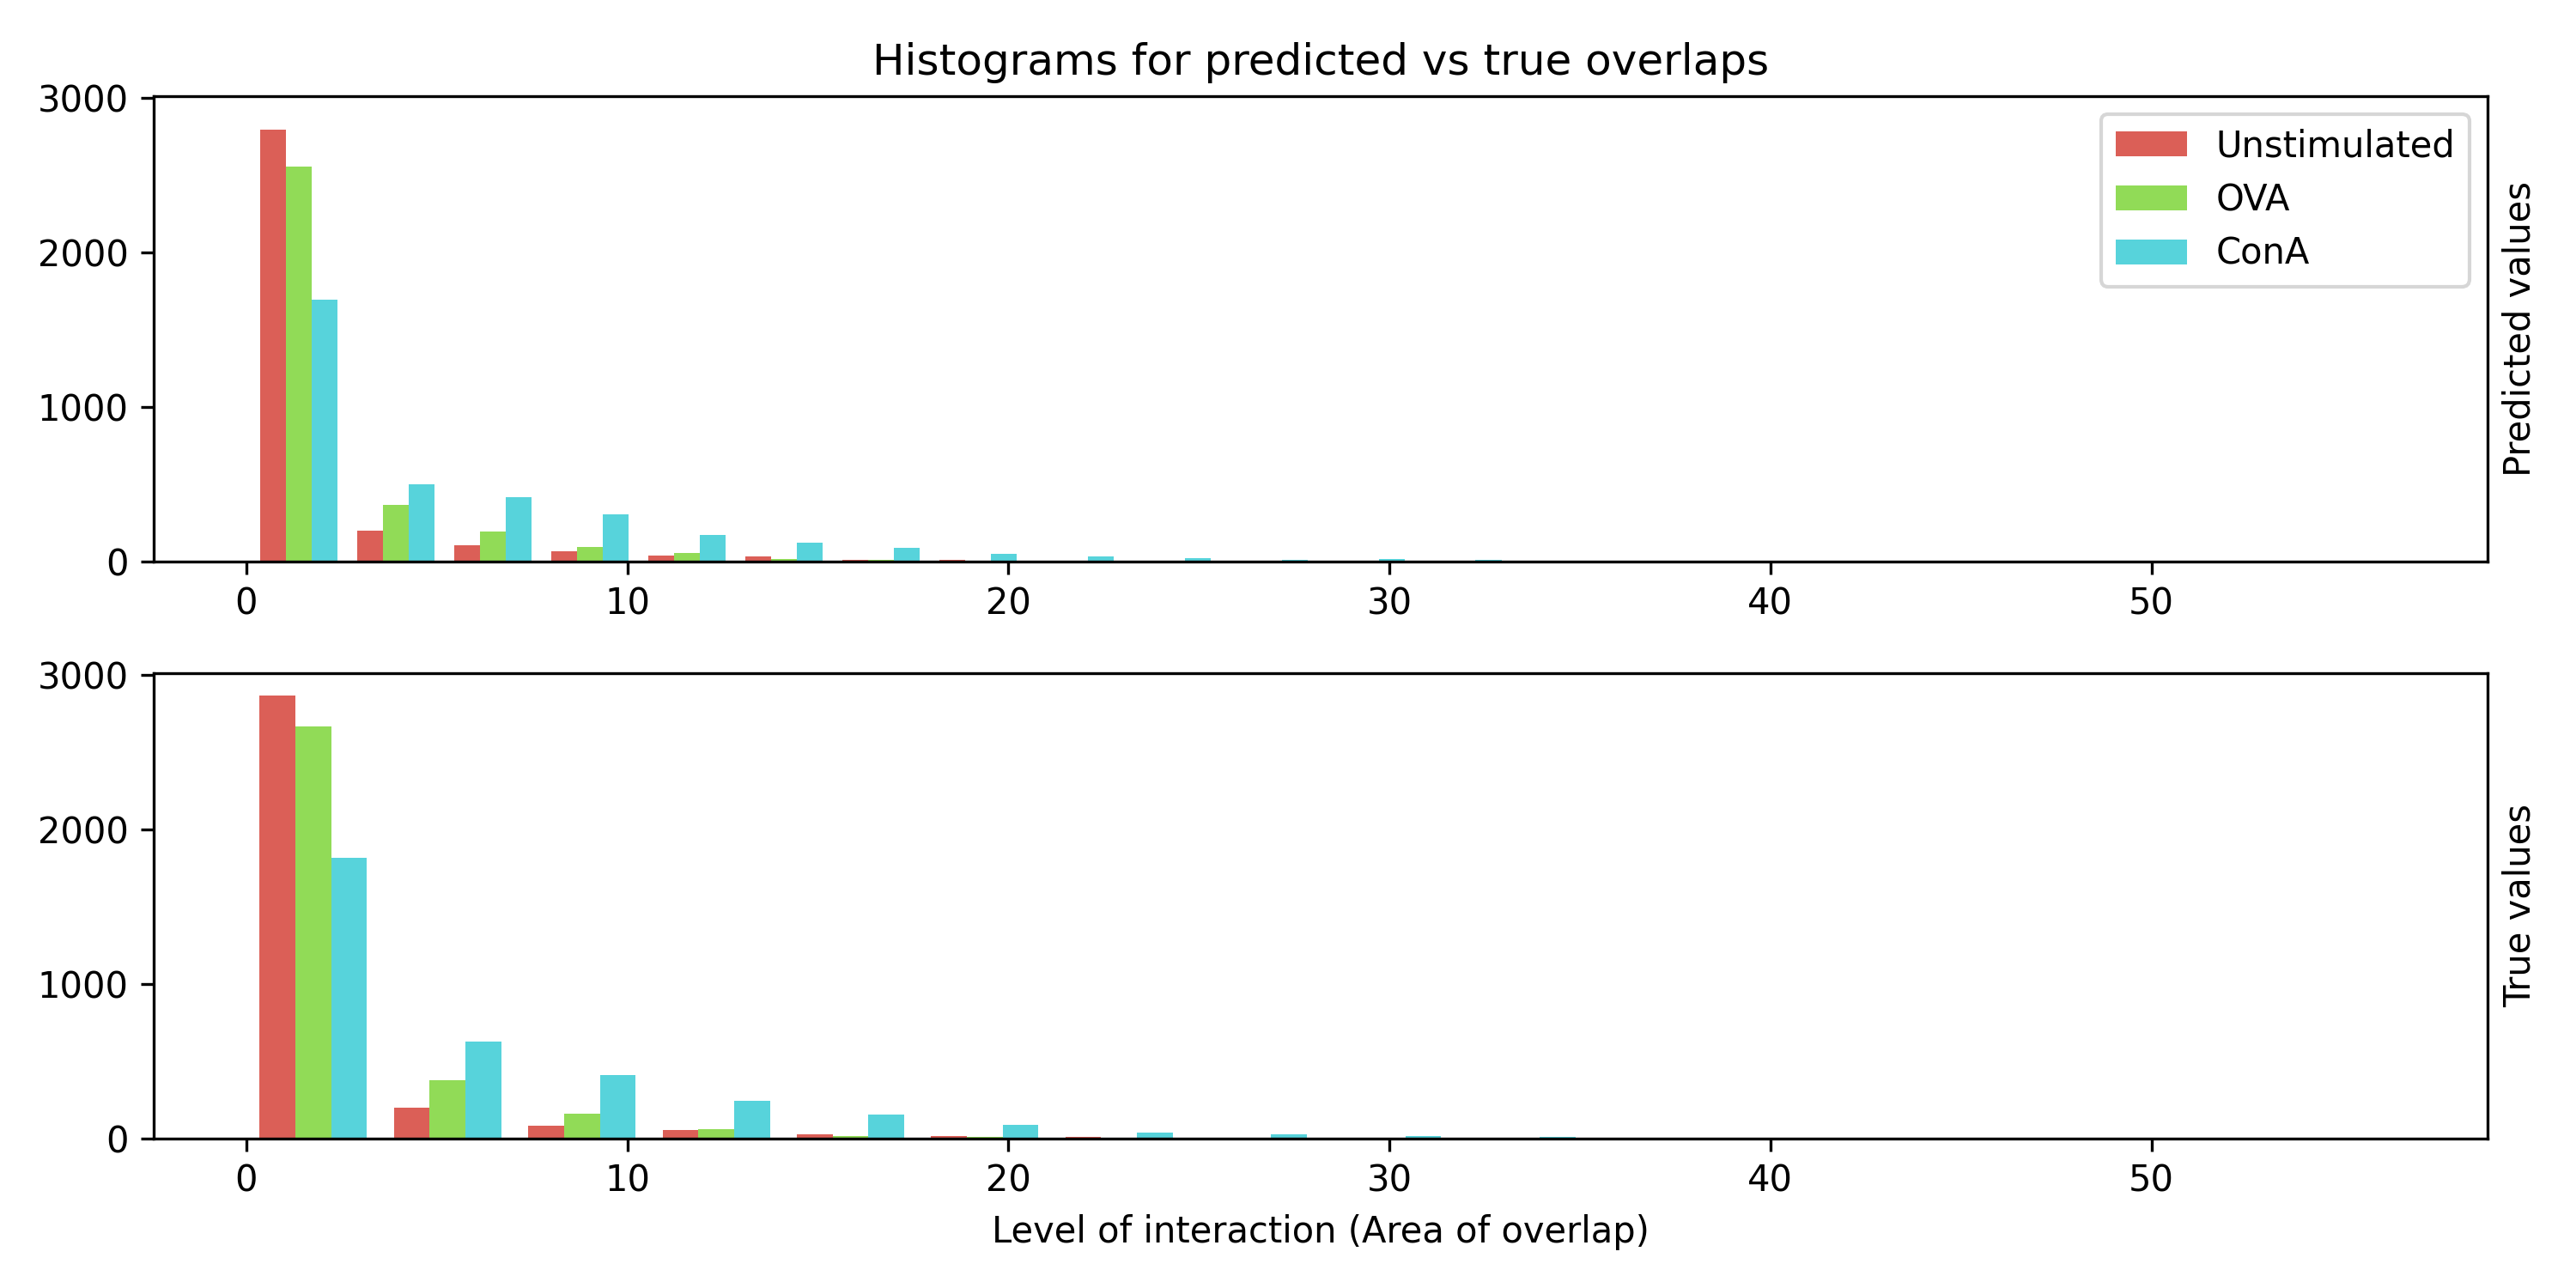
\includegraphics[width=.8\textwidth]{dissertation/figures/evaluation/CK19_histogram.png}
    \caption{Histogram showing the distribution of overlap values for each stimulation category. The true values are at the bottom, and the predicted values for the normal dataset are at the top. Most images have an overlap value of around 0, and images in the ConA category show the biggest overlaps.}
    \label{fig:full_histogram}
\end{figure}

To illustrate this, we show the distribution of the true and predicted values of overlap between immune cells in the images in a histogram in Figure \ref{fig:full_histogram}. The true distribution of overlap values highlights that there are a lot more of overlap values distributed around 0 for the \textit{Unstimulated} and \textit{OVA} categories. 

Nonetheless, the RMSE scores for our masked regression model are much more promising. This is also reflected in the scatter plots. Figure \ref{fig:full_masked_scatter} shows that in comparison to the normal model, predicted values for the masked model follow the line of best fit much closer. 

\bigskip
\subsubsection{Dual dataset}
\hfill
\hfill 

Regression performance on the unseen dual dataset was similar as to above. Overall, it achieved lower scores of RMSE with general scores of 1.677 $\pm$ 3.183 for the normal model and 0.932 $\pm$ 3.456 for the masked model. The SD of the true values is of 3.626 overall, hence we can say the predictions represent the variability of the true values. The RMSE scores need to be put into contrast with the fact that in the full dataset, the \textit{ConA} category had higher RMSE scores due to having a distribution with higher overlap values. \autoref{tab:dual_rmse} reports the full RMSE and SD scores. Compared to \autoref{tab:full_rmse} above, the regression model achieved a similar performance on the unseen dataset for images in the \textit{Unstimulated} category. 

\begin{table}[h!]
\centering
\caption{Average RMSE and SD scores (in \%) for the regression model's predictions on the \textbf{dual} dataset. The closer the value is to 0, the closer the prediction is. There is an improvement in RMSE score in the masked model, and it accounts for more variance in the data.}
\label{tab:dual_rmse}
\begin{tabular}{l|rr|r}
\rowcolor[HTML]{EFEFEF}
\textbf{Images} & \cellcolor[HTML]{FFCCC9}\textbf{Unstimulated} & \cellcolor[HTML]{C9FFCB}\textbf{OVA} & \textbf{All} \\ \hline
Normal      & 1.233 $\pm$ 1.981  & 2.026 $\pm$ 3.898  &   1.677 $\pm$ 3.183  \\ \hline
Masked      &    0.673 $\pm$ 2.265   &  1.133 $\pm$ 4.310   &   0.932 $\pm$ 3.456 
\end{tabular}
\end{table}

\begin{figure}[bh!]
    \centering
    \begin{subfigure}{0.5\textwidth}
        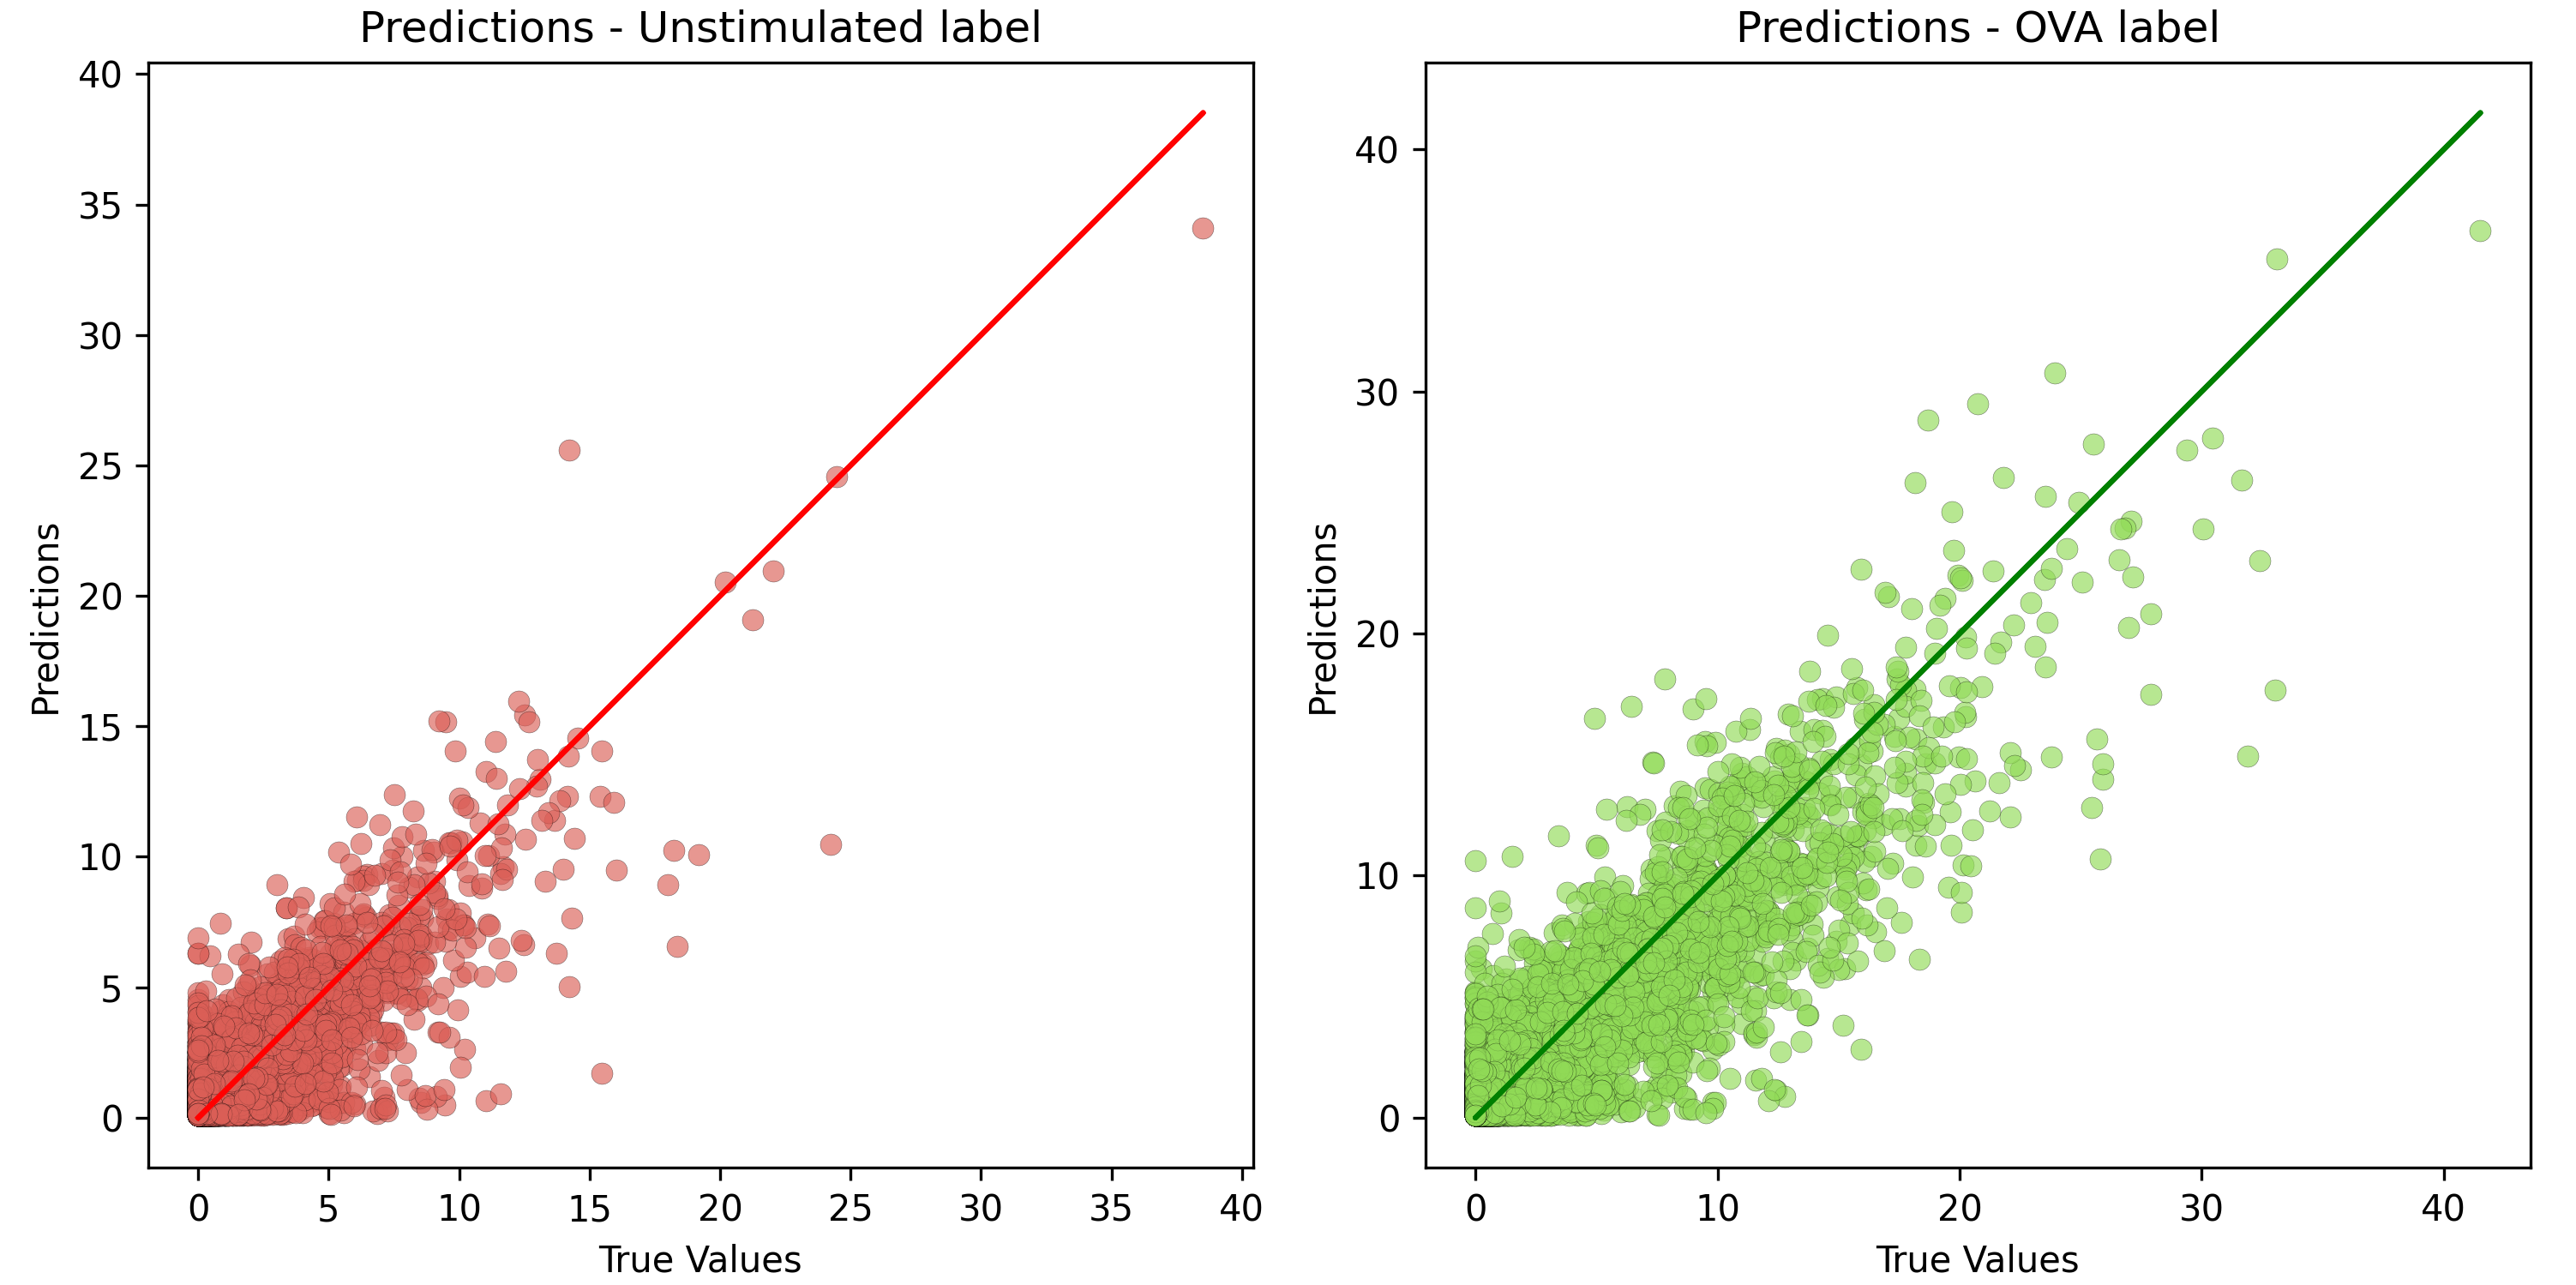
\includegraphics[width=\textwidth]{dissertation/figures/evaluation/CK22_scatter.png}
        \caption{Normal images}
    \end{subfigure}
    \begin{subfigure}{0.5\textwidth}
        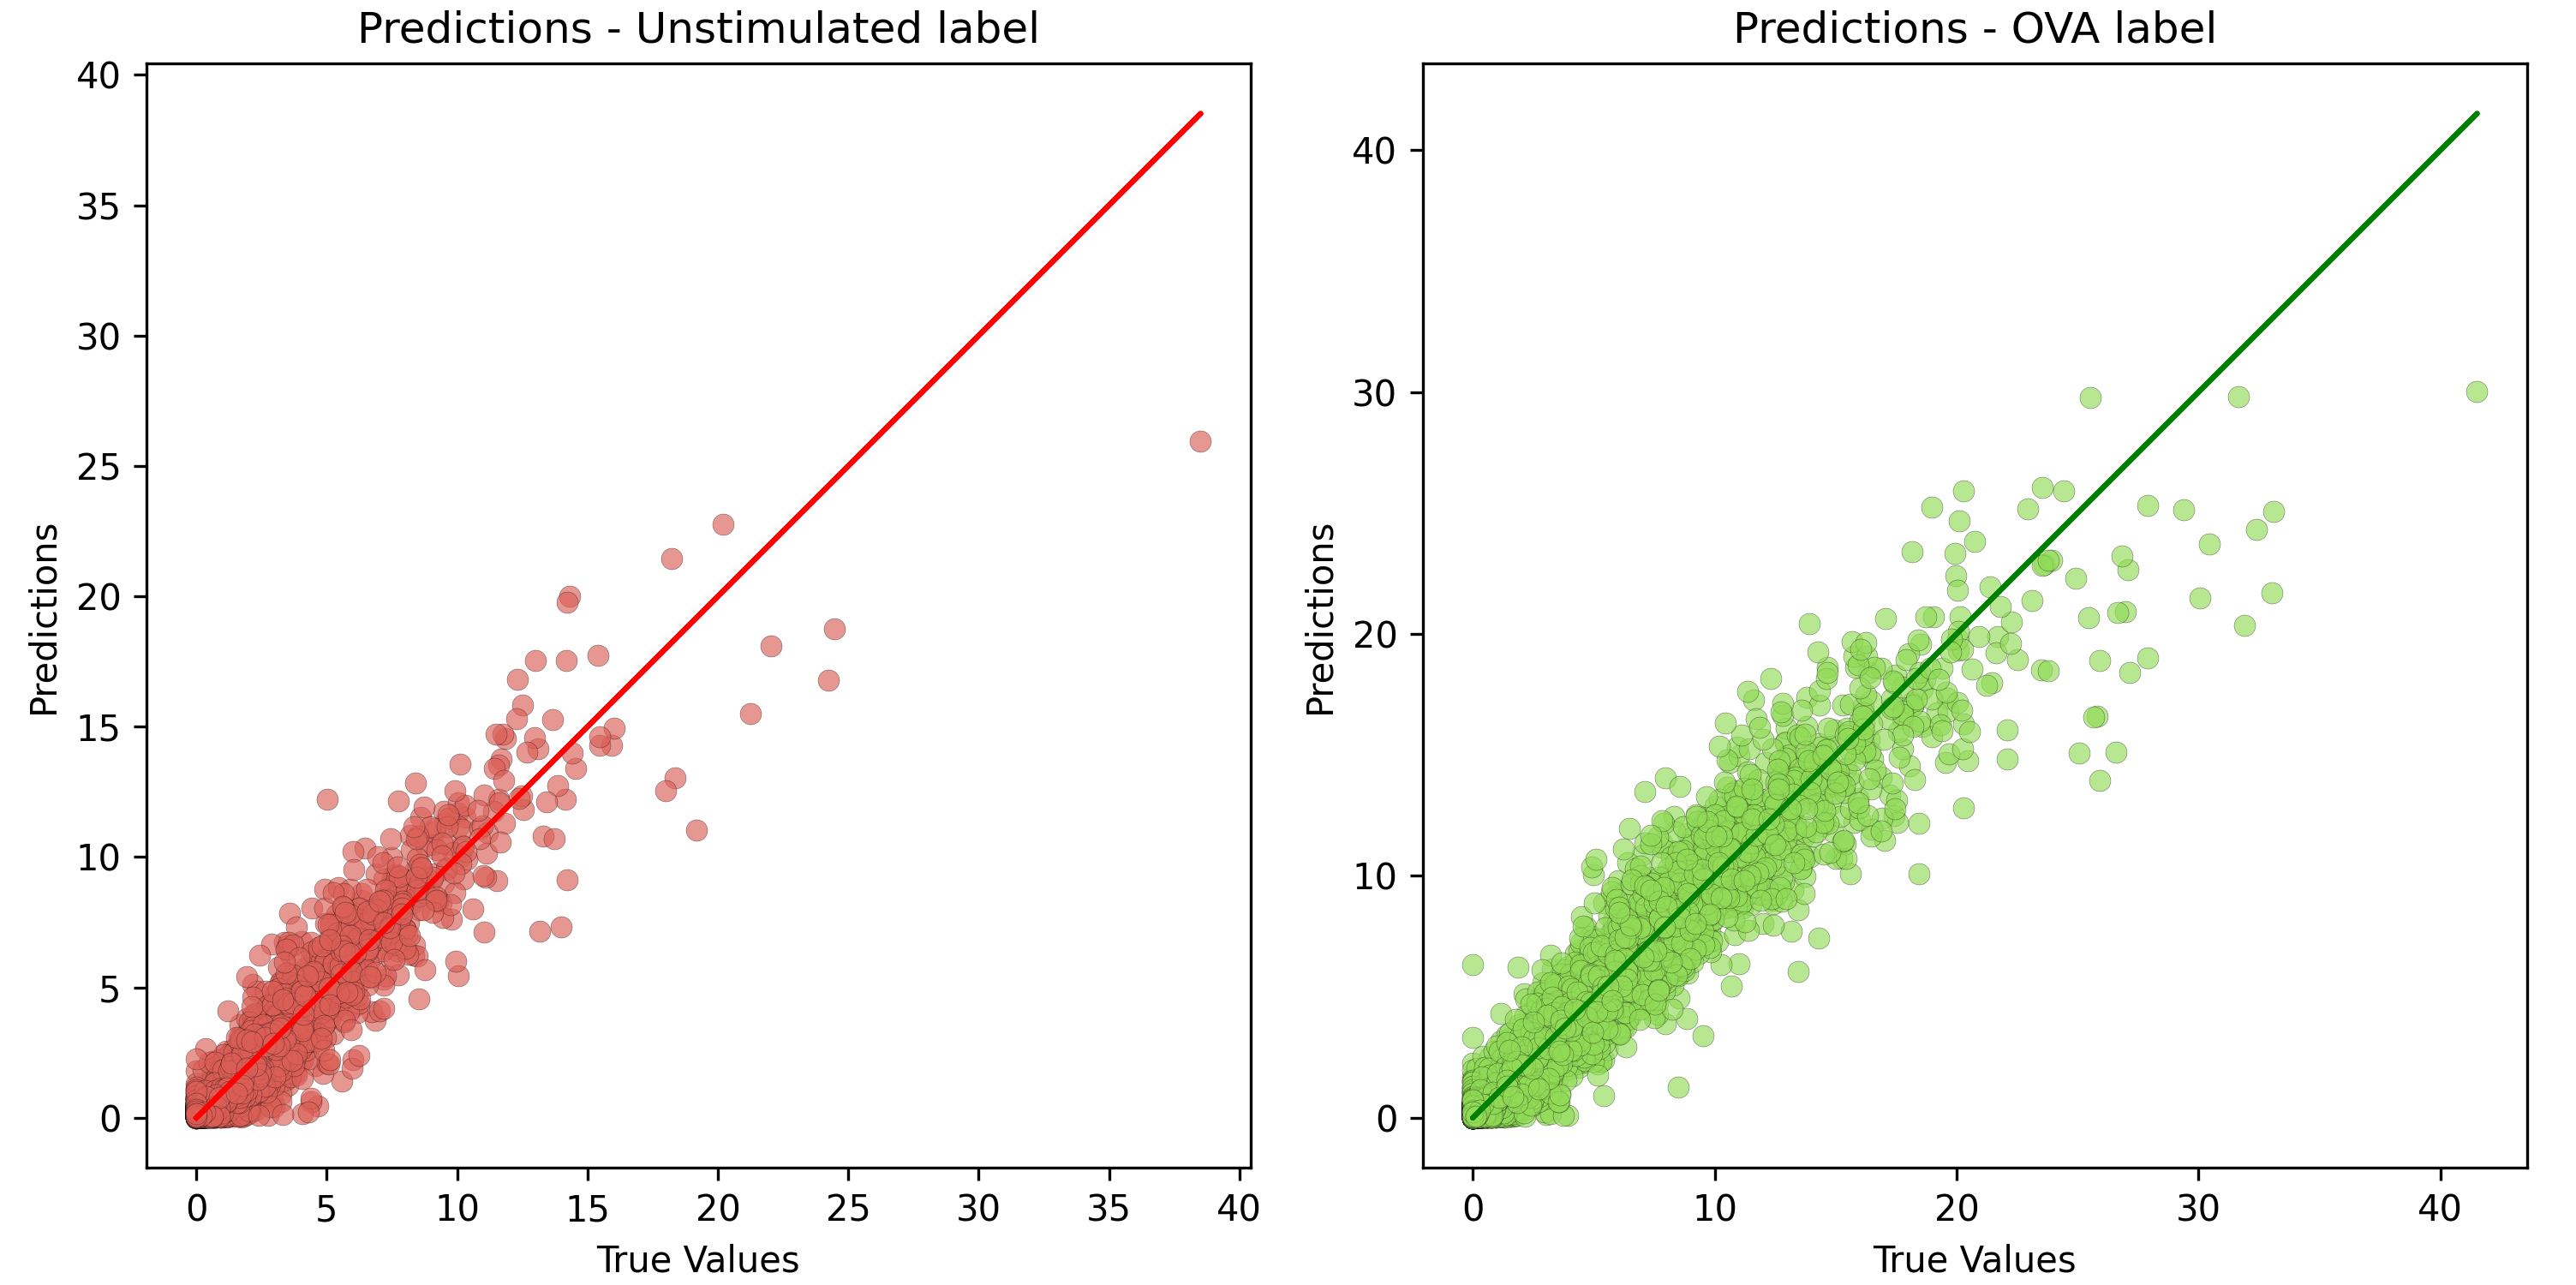
\includegraphics[width=\textwidth]{dissertation/figures/evaluation/CK22_masked_scatter.png}
        \caption{Masked images}
    \end{subfigure}
    \caption{Scatter plot comparing true values (x-axis) to predicted values (y-axis) for the \textbf{dual} dataset. The line of best fit is the straight continuous line running diagonally true the plot, which is the line we want our predictions on. The normal regression models performs rather poorly around overlap values of 0, in both categories.}
    \label{fig:dual_scatter}
\end{figure}

\autoref{fig:dual_scatter} shows how the predictions are positioned around the line of best fit for this dataset. We can see that predictions are poor around 0: the model predicts values too high for true values of 0, and predicts values too close to 0 for values much higher. For example, a true value of close to 15\% overlap was predicted as close to 0\% overlap as shown in the \textit{Unstimulated} graph. Predictions also become poorer towards higher values, for both normal and masked images.

\bigskip
\subsubsection{DMSO dataset}
\hfill
\hfill 

For the regression task, we are not comparing images of different categories, but trying to predict an interaction value from an image. As such, we were hoping that the \textbf{DMSO} dataset would have similar performance as the \textbf{full} dataset, as class imbalance issues should be less significant. 

The regression model achieved an overall score of 1.837 $\pm$ 3.816 for the normal model, and 1.161 $\pm$ 4.732 for the masked model. SD of the true values is of 4.405 overall. Again, we see an improvement in scores in the masked model. Full scores are reported in \autoref{tab:dmso_rmse}. As expected, performance is similar across all categories compared to the full dataset, with the \textit{OVA} category showing the most difference. 

\begin{table}[h!]
\centering
\caption{Average RMSE and SD scores (in \%) for the regression model's predictions on the \textbf{DMSO} dataset. The closer the value is to 0, the closer the prediction is. We again observe an improvement in the RMSE score in the masked model, and it accounts for variance in the data closer to the true SD value of 4.405.}
\label{tab:dmso_rmse}
\begin{tabular}{l|rrr|r}
\rowcolor[HTML]{EFEFEF}
\textbf{Images} & \cellcolor[HTML]{FFCCC9}\textbf{Unstimulated} & \cellcolor[HTML]{C9FFCB}\textbf{OVA} & \cellcolor[HTML]{96FFFB}\textbf{ConA} & \textbf{All} \\ \hline
Normal      & 1.013 $\pm$ 1.945  & 2.202 $\pm$ 4.308   & 2.567 $\pm$ 4.720  &   1.837 $\pm$ 3.816  \\ \hline
Masked      &    0.700 $\pm$ 2.147          & 1.199 $\pm$ 4.809  &  1.773 $\pm$ 4.665   &   1.179 $\pm$ 4.011 
\end{tabular}
\end{table}

\begin{figure}[h!]
    \centering
    \begin{subfigure}{0.8\textwidth}
        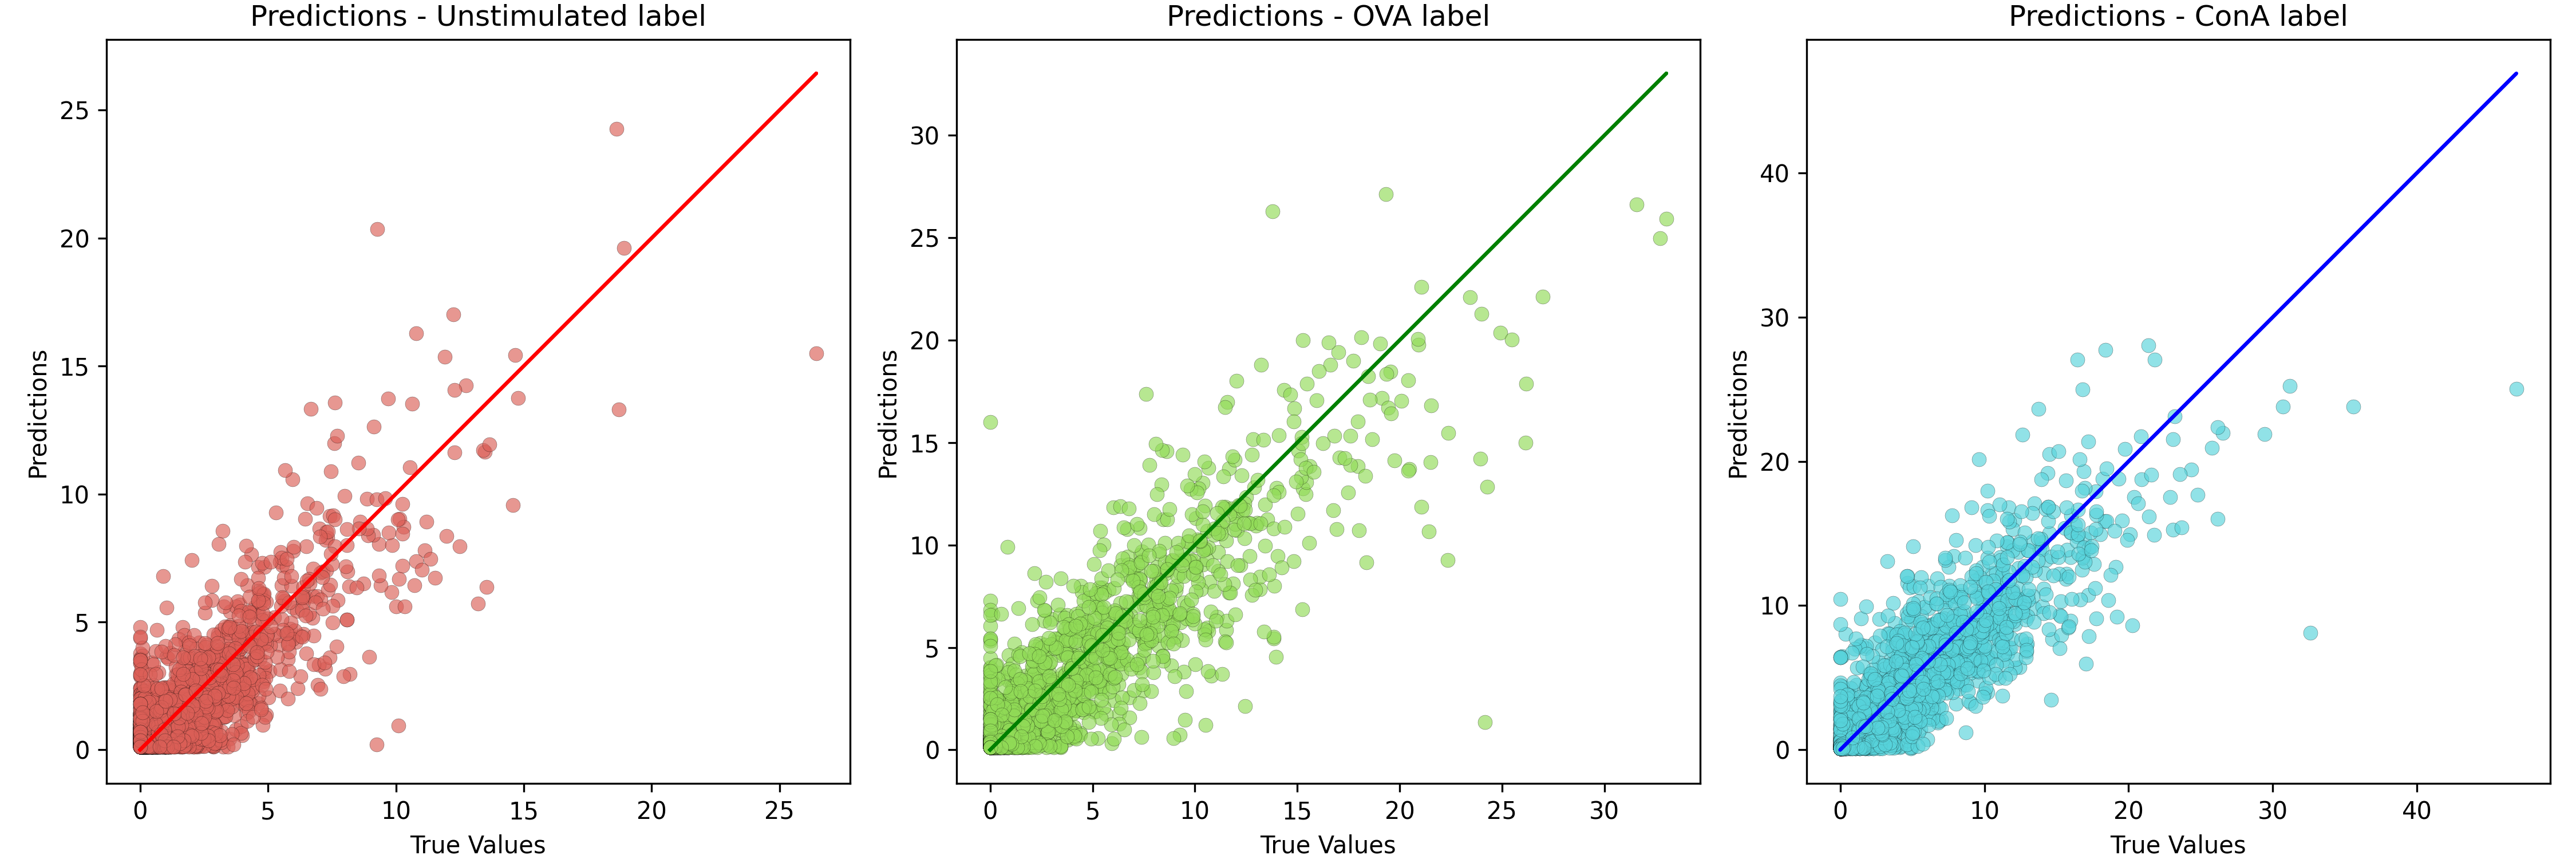
\includegraphics[width=\textwidth]{dissertation/figures/evaluation/DMSO_scatter.png}
        \caption{Normal images}
    \end{subfigure}
    \begin{subfigure}{0.8\textwidth}
        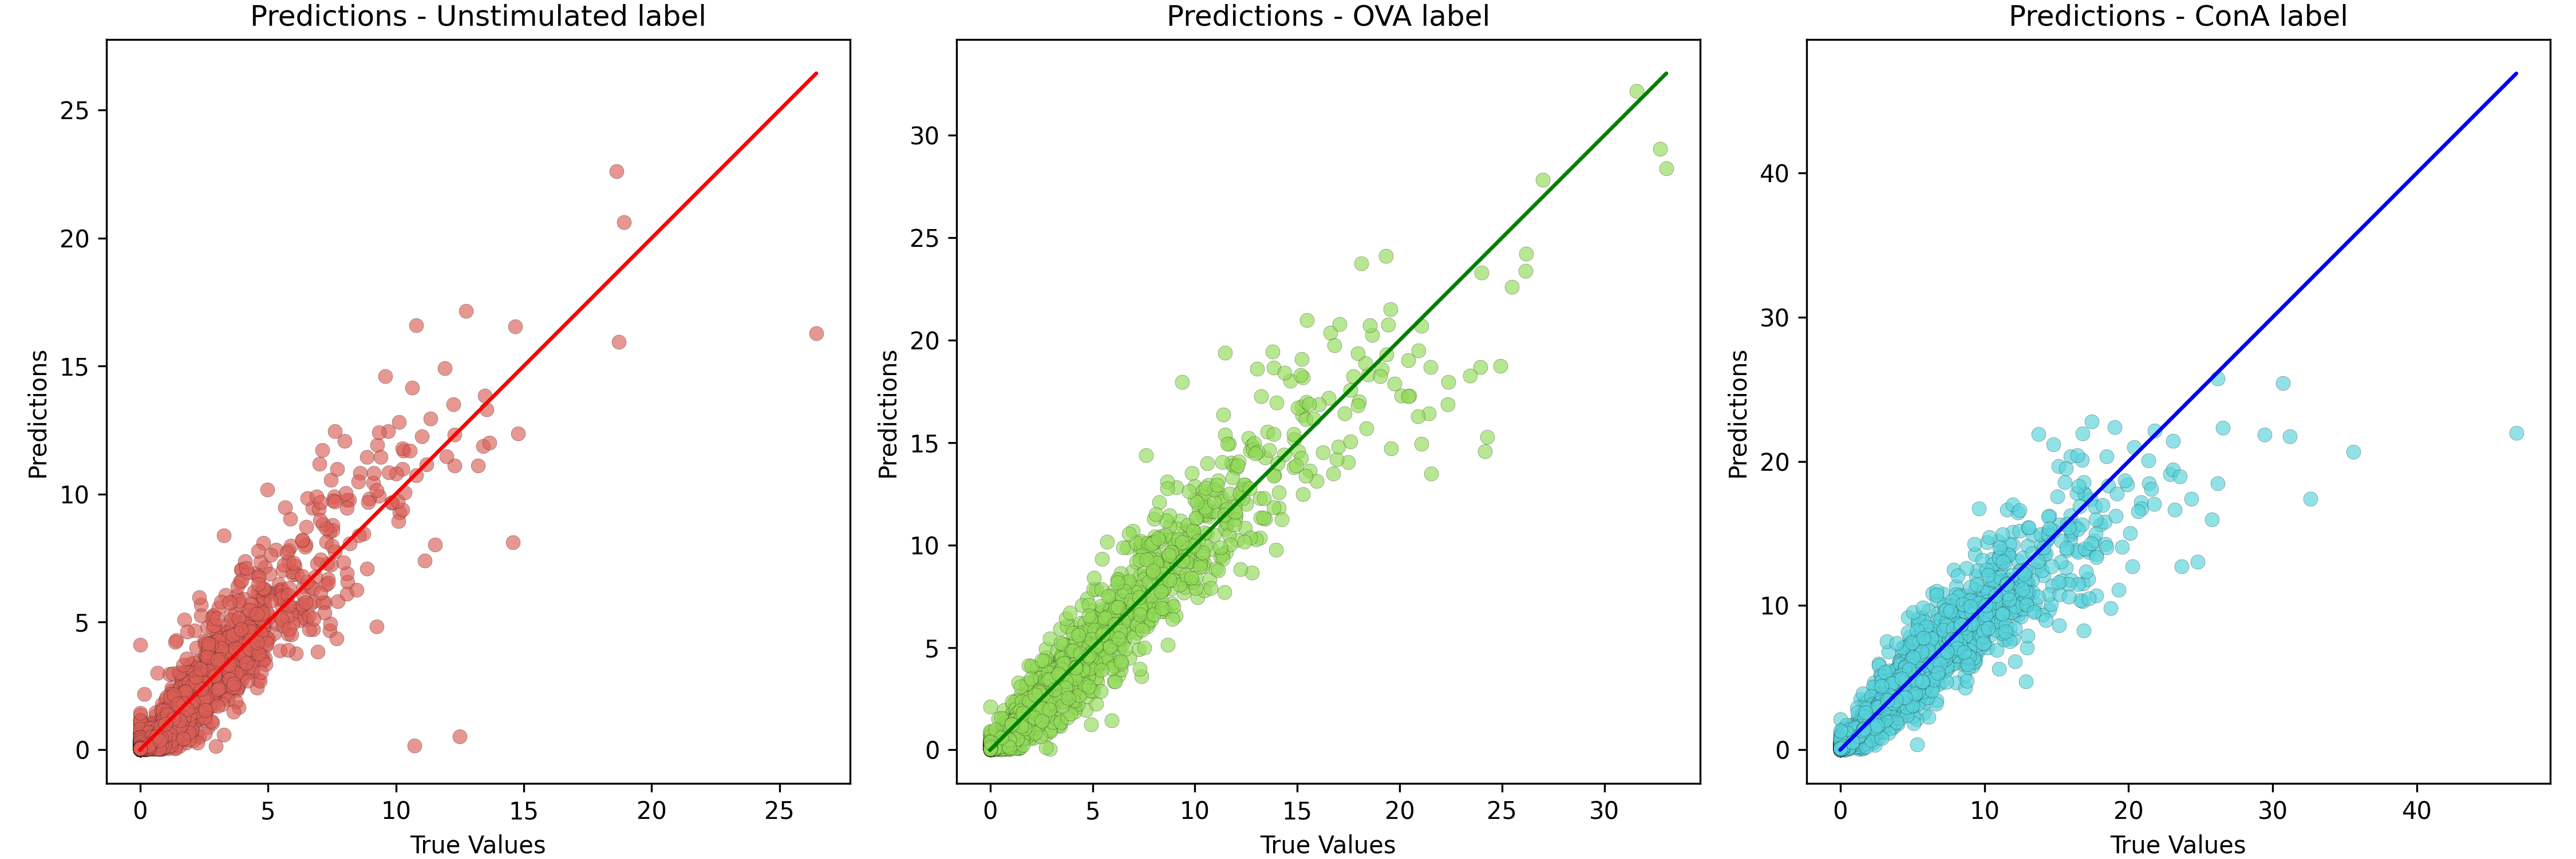
\includegraphics[width=\textwidth]{dissertation/figures/evaluation/DMSO_masked_scatter.png}
        \caption{Masked images}
    \end{subfigure}
    \caption{Scatter plot comparing true values (x-axis) to predicted values (y-axis) for the \textbf{DMSO} dataset. The line of best fit is the straight continuous line running diagonally true the plot, which is the line we want our predictions on. For both the normal and masked models, there seems to be some large errors around higher values of overlap. Each sub-plot is not on the same scale as each category does not have the same range of overlap values, but we wanted to show more granularity for each sub-plot.}
    \label{fig:dmso_scatter}
\end{figure}

The scatter plot showing the line of best fit is available in \autoref{fig:dmso_scatter}. Similarly to the dual dataset, we can see that there is a higher variation around predictions of higher values in both types of images. This might signify that our regression model is struggling with higher values of overlap. 

\section{Discussion}

In this section we have shown the results of the development of our autoencoder and regression models. These results have shown that convolutional autoencoders can reconstruct images of immune cells well with a highest binary cross-entropy loss of 0.1159 and a lowest score of 0.0156. The autoencoder also sped up the process of high-dimensional data projection from an hour to minutes, which is particularly significant for the field of immunology where imaging data is predominantly high dimensional. Moreover, it was an efficient building block to extract features from images to be passed onto fully connected layers for a regression task. Indeed, our deep regression model has shown good results with the highest average RMSE score being 1.838 (\%). Particularly, we have noticed that the correct pre-processing of images, particularly the removal of noisy backgrounds, greatly helps a model's learning.

The results also have implications for the analysis of interaction between immune cells. From what we observed here, we can say that deep learning methods are suited for the task of processing images of immune cells. We were able to train a consistent regression model for the task of predicting overlap value from an image of immune cells, where we assumed more overlap meant more interaction between immune cells. This method can be faster on GPUs for obtaining metrics from images rather than segmenting images and calculating overlaps directly.

We were not able to uncover an underlying structure to the data with the help of the autoencoder. However, there could be multiple reasons for this as our evaluation had limitations. The difference between DMSO-only results and the results on the other datasets tells us that the experimental conditions behind each image did have an impact on their structure. This is significant as it highlights that microscope images will have to be carefully selected and processed in order to yield results suited for analysis. Datasets should be built around precise experimental conditions to best exploit the capabilities of deep learning models. For example, a dataset could be built from images of immune cells taken from the same stimulation category, but labelled by drug compound used. It is also worth noting that the results here were obtained with image patches of size $192\times192$. This gives quite a local view of the cells, and a bigger window size could give a more global view and as such more information about how different cells behave together. Therefore the size of the sub-images should also be taken in consideration, as it might yield different results. 

%An autoencoder could then be used to reduce the dimensionality of the images and analyse the structure of the images with UMAP to observe any clusters. A similar regression model could also be used with a metric of choice to infer levels of interaction from images. 